%% Template for EU deliverable, using the deliverable.sty style file

\documentclass[12pt,a4paper,twoside]{report}

%% common package
\usepackage[headers]{deliverable}
\usepackage{xspace}
\usepackage{verbatim}
\usepackage[usenames]{color}
\usepackage{listings}
\usepackage[usenames,dvipsnames,table]{xcolor}
\usepackage[pdftex,dvips]{graphicx}
\usepackage{url}
\usepackage{array}

%%

%%%%%%%%%%%%%%%%%%%%%%%%%%%%%%%%%%%%%%%%%%%%%%%%%%%%%%%%%%%%%%%%%%%%%%%%%%%%%%
%%% Misc. packages
%%%%%%%%%%%%%%%%%%%%%%%%%%%%%%%%%%%%%%%%%%%%%%%%%%%%%%%%%%%%%%%%%%%%%%%%%%%%%%
\usepackage[]{nomencl}		% nomenclatures
\graphicspath{{./figure/}}
\usepackage{pdfpages}
\usepackage{amsmath} % assumes amsmath package installed
\usepackage{amssymb}  % assumes amsmath package installed
\usepackage{mathtools}
\usepackage{graphicx}
\usepackage{hyperref}
\hypersetup{
	bookmarks=true,         % show bookmarks bar?
	unicode=false,          % non-Latin characters in Acrobat’s bookmarks
	pdftoolbar=true,        % show Acrobat’s toolbar?
	pdfmenubar=true,        % show Acrobat’s menu?
	pdffitwindow=false,     % window fit to page when opened
	pdfstartview={FitH},    % fits the width of the page to the window
	pdfkeywords= {}, % list of keywords
	pdfnewwindow=true,      % links in new window
	colorlinks=true,       % false: boxed links; true: colored links
	linkcolor=black,          % color of internal links (change box color with linkbordercolor)
	citecolor=black,        % color of links to bibliography
	filecolor=black,      % color of file links
	urlcolor=black           % color of external links
}

%%%%%%%%%%%%%%%%%%%%%%%%%%%%%%%%%%%%%%%%%%%%%%%%%%%%%%%%%%%%%%%%%%%%%%%%%%%%%%
%%% Luka's packages
%%%%%%%%%%%%%%%%%%%%%%%%%%%%%%%%%%%%%%%%%%%%%%%%%%%%%%%%%%%%%%%%%%%%%%%%%%%%%%
\usepackage{cite}
\usepackage{mathptmx} % assumes new font selection scheme installed
\usepackage{bm,times} % assumes new font selection scheme installed
\usepackage{amsfonts}
\usepackage{stfloats}
\usepackage{psfrag}
\usepackage{float}
\usepackage{color}

%%%%%%%%%%%%%%%%%%%%%%%%%%%%%%%%%%%%%%%%%%%%%%%%%%%%%%%%%%%%%%%%%%%%%%%%%%%%%%
%%% Serena's packages
%%%%%%%%%%%%%%%%%%%%%%%%%%%%%%%%%%%%%%%%%%%%%%%%%%%%%%%%%%%%%%%%%%%%%%%%%%%%%%
\pdfoutput=1

\RequirePackage{fix-cm}
\usepackage{multicol}
\usepackage{xcolor,colortbl}
\usepackage{wrapfig}
\usepackage{mdwtab} %added by Na
\usepackage{mdwmath}
\usepackage{enumerate}
\usepackage{algorithm2e}
\usepackage[utf8]{inputenc}
\usepackage{caption}



%%%%%%%%%%%%%%%%%%%%%%%%%%%%%%%%%%%%%%%%%%%%%%%%%%%%%%%%%%%%%%%%%%%%%%%%%%%%%%
%%% Titlepage
%%%%%%%%%%%%%%%%%%%%%%%%%%%%%%%%%%%%%%%%%%%%%%%%%%%%%%%%%%%%%%%%%%%%%%%%%%%%%%

% declaration of variables used in style
\deliverableDocnumber{D2.3}
\deliverableTitle{Models of systematic application of physical interaction with the environment and humans}

\deliverableAuthor{Jernej \v{C}amernik$^{1}$, and Jan Babi\v{c}$^{1}$}
\deliverableResponsiblePartner{JSI}
\deliverableAffiliation{$^1$ Department for Automation, Biocybernetics and Robotics, Jo\v{z}ef
  Stefan Institute, Ljubljana, Slovenia.}

\deliverableReviewer{}
\deliverableCoordinator{Jan Babi\v{c}}
\deliverableActivityNumber{n} %% n=1,..,10
\deliverableActivity{Activity Name}
\deliverableDoctype{Deliverable} %% or Prototype
\deliverableClassification{Public} % or Consortium
\deliverableDistribution{Consortium} %
\deliverableStatus{Final} % Draft or Final
\deliverableDeliveryDate{28/2/2017}
\deliverableFile{D2.3\D2.3.pdf} % please do not use "-" in the name
\deliverableVersion{1.0}
\deliverableDate{28/2/2017}
\deliverableYear{2017}
\deliverablePages{\pageref{LastPage}}
\deliverableChangelog{v.0.1 & Feb 15, 2017 & Initial draft %%\\\hline
%%              v.2.0 & Feb 20, 2007 & Final version
}
\deliverableProjectStartingDate{1st March 2013}
\deliverableProjectEndDate{28th February 2017}
\deliverableProjectAcronym{CoDyCo}
\deliverableProjectTitle{Whole-Body Compliant Dynamical Contacts in Cognitive Humanoids}
\deliverableContractNumber{600716}
\deliverableProjectCoordinator{Istituto Italiano di Tecnologia}
\deliverableProjectUrl{www.codyco.eu}
\deliverableFrameworkProgramme{FP7}

\deliverableWorkpackage{WP2}
\deliverableEditors{Jernej \v{C}amernik, and Jan Babi\v{c}}
\deliverableContributors{Serena Ivaldi (INRIA), Chie Takahashi (UB), Zrinka Potocanac (JSI), Luka Peternel (JSI), Jan Babi\v{c} (JSI)}
\deliverableReviewers{}
\deliverableAbstract{The scope of the current deliverable is to present the
  results on developing models of human whole body motions in contact with
  environment.}
\deliverableKeywordList{contacts, model learning, probabilistic movement
  representations}


%%%%%%%%%%%%%%%%%%%%%%%%%%%%%%%%%%%%%%%%%%%%%%%%%%%%%%%%%%%%%%%%%%%%%%%%%%%%%%
%%% Sections
%%%%%%%%%%%%%%%%%%%%%%%%%%%%%%%%%%%%%%%%%%%%%%%%%%%%%%%%%%%%%%%%%%%%%%%%%%%%%%

%% constants
\newcommand{\botegoCaps}{BOTEGO}
\newcommand{\certhCaps}{CERTH}
\newcommand{\cybionCaps}{CYBION}
\newcommand{\nuigCaps}{NUIG}
\newcommand{\ubitechCaps}{UBITECH}

% Chie
\newcommand{\BF}{\mathbf{F}}
\newcommand{\BZ}{\mathbf{Z}}
\newcommand{\BA}{\mathbf{A}}
\newcommand{\BB}{\mathbf{B}}
\newcommand{\BC}{\mathbf{C}}
\newcommand{\BD}{\mathbf{D}}
\newcommand{\BW}{\mathbf{W}}
%%
%%%%%%%%%%%%%%%%%%%%%%%%%%%%%% BEGIN DOCUMENT
\begin{document}

\deliverableMaketitle

%%TODO move to style
\newcolumntype{L}[1]{>{\raggedright\let\newline\\\arraybackslash\hspace{0pt}}m{#1}}
\newcolumntype{C}[1]{>{\centering\let\newline\\\arraybackslash\hspace{0pt}}m{#1}}
\newcolumntype{R}[1]{>{\raggedleft\let\newline\\\arraybackslash\hspace{0pt}}m{#1}}

\textbf{Document Revision History}
\begin{center}
\begin{tabular}{|C{2cm}|C{3cm}|p{5cm}|C{4cm}|}
\hline
\textbf{Version}&\textbf{Date}&\textbf{Description}&\textbf{Author}\\\hline
v. 1.0 & 28 Feb 2017 & Final Version & Jernej \v{C}amernik\\\hline
\end{tabular}
\end{center}
 
 \clearpage

\newpage
\renewcommand*\contentsname{Table of Contents}
%\renewcommand*\listfigurename{Index of Figures}
\tableofcontents
\newpage
%\listoffigures
%\newpage

%%%%%%%%%%%%%%%%%%%%%%%% Start deliverable content here.

\chapter{Introduction}\label{sec:Intro}
%Short summary of our collaborative contribution
This deliverable reports on adaptive models describing changes in human whole body motion in contact with unpredictable support surfaces and humans. The goal of the work reported in this deliverable was to understand the factors involved in human choice of contact utilization and to investigate how interaction through contacts can contribute to learning of whole body motor control. There are numerous situations where humans utilize physical interaction with either the environment or another human to stabilise one’s own balance. These can be through light touch to gain additional haptic information from the environment; through weight-bearing support; through energy storage and recovery from a springy surface; and through assistive forces from other humans. In this regard we investigated how human physical interactions with rigid, compliant or spring-like contacts contribute to changes in whole body motion and to task-relevant parameters. The core question that we addressed is how a human can learn to predict the environmental properties by performing tasks with hand or body contacts and then generalize the learned predictive mechanisms to other tasks. For example, does interaction with the support surface during a supported reaching action allow effective choice of and use of the support? The findings reported in this deliverable are models that can be further used to enhance robot-learning capabilities by systematic application of physical interaction with the environment or humans.
\bigskip

In Chapter \ref{sec:Chie} we summarize the work of exploring the mechanism which helps humans to learn the compliant force dynamics. This mechanism enables us to get an in-depth understanding of how humans modulate whole-body motion to reach anticipated goals ruled by the external force. Further, this is beneficial to apply it for controlling the humanoid robot in order to keep a stable posture when interacting with multiple compliant surfaces. With reference to the results of the pilot experiment (see the D2.2), the experimental design has been developed and human subject experiments were conducted to examine the human learnability factor in different force dynamics. Three different types of forces (simple linear and two non-linear forces) were generated and the human movements to reach the anticipated goal were measured against the compliant forces.
\bigskip

In Chapter \ref{sec:Serena} we address the human - robot interaction as estimating the engagement is critical. Engagement measures typically rely on the dynamics of the social signals exchanged by the partners, especially speech and gaze. However, the dynamics of these signals is likely to be influenced by individual and social factors, such as personality traits, as it is well documented that they critically influence how two humans interact with each other. Here, we assess the influence of two factors, namely extroversion and negative attitude toward robots, on speech and gaze during a cooperative task, where a human must physically manipulate a robot to assemble an object. We evaluate if the score of extroversion and negative attitude towards robots co-variate with the duration and frequency of gaze and speech cues. The experiments were carried out with the humanoid robot iCub and N=56 adult participants. We found that the more people are extrovert, the more and longer they tend to talk with the robot; and the more people have a negative attitude towards robots, the less they will look at the robot face and the more they will look at the robot hands where the assembly and the contacts occur. Our results confirm and provide evidence that the engagement models classically used in human-robot interaction should take into account attitudes and personality traits.
\bigskip

In Chapter \ref{sec:Luka} we propose a novel method that arbitrates the control between the human and the robot actors in a teaching-by-demonstration setting to form synergy between the two and facilitate effective skill synthesis on the robot. We employed the human-in-the-loop teaching paradigm to teleoperate and demonstrate a complex task execution to the robot in real-time. As the human guides the robot to perform the task, the robot obtains the skill online during the demonstration. To encode the robotic skill we employed Locally Weighted Regression that fits local models to specific state region of the task based on the human demonstration. If the robot is in the state region where no local models exist, the control over the robotic mechanism is given to the human to perform the teaching. When local models are gradually obtained in that region, the control is given to the robot so that the human can examine its performance already during the demonstration stage, and take actions accordingly. This enables a co-adaptation between the agents and contributes to a faster and more efficient teaching. As a proof-of-concept, we realised the proposed robot teaching system on a haptic robot with the task of generation of a desired vertical force on a horizontal plane with unknown stiffness properties.
\bigskip

In Chapter \ref{sec:Zrinka} we present preliminary results from a study which is a follow-up of the previous work (presented in D2.2) which showed how contacts are established to facilitate goal directed movements. Here we ask an inverse question: how would a contact be released? Furthermore, if there is an uncertainty of balance (in our case elicited by perturbing balance with an underlying Stewart platform), how does this contact preference change? As a model for this behavior we used stepping to a target from quiet stance. In this case, in order to execute a goal directed movement (step onto the target), one first has to break a stabilizing contact of the foot with the ground. We found that manipulating balance by systematic platform movements delayed step onsets, i.e., prolonged the time needed before the supporting contact was broken. We also investigated the effect of balance uncertainty and task difficulty on feed-forward and feedback control of stepping by analyzing stepping  accuracy. Together with the pending analysis of how such behaviors develop and adapt to environmental demands, these findings will be further used to help the robot controller when the robot has joint torque limits, joint position limits, or narrow stability margins. In effect, these models will help the robot decide when to make or break the contacts.

% \chapter{Executive Summary}

\newpage{}
\chapter{Compliant-contact force perception study}\label{sec:Chie}
\setcounter{figure}{0}

%%%%%%%%%%%%%%%%%%%%%%%%%%%%%%%%%%%%%%%%%%%%%%%%%%%%%%%%%%%%%%%%%%%%%%%%%%%%%%%%
\section{Introduction}

Studying human strategies of dealing with uncertain contact is important to formulate equivalent humanoid robot behaviour, in particular with multiple non-rigid contacts. In the real-world interactions, there are varied and complicated force dynamics (i.e., governed by not only simple linear principles) when making a contact with an object and handling it. Humans can learn a new force dynamics through sensorimotor learning and adaptation, and they can control their whole body movements to the desired contact in an uncertain environment. The CNS (Central Nervous System) seems to generalise the dynamics through visuomotor learning, and the formalisation enables humans to predict the consequence of action and to achieve the behavioural goal optimally \cite{Wolpert2011, Davidson2003}. Previous studies have shown that a certain exposure (repetitive movements) against forces facilitates to learn the spatial and temporal characteristics of the interaction via error-based visuomotor perturbation paradigm \cite{Goodbody1998, Krakauer2006}. Humans likely generalize the force principles in a cognitively robust way and optimise their body movements interacting with the force. However, the detailed process and the underlying mechanisms are little unknown.

Like humans, robots are required to flexibly adjust their posture and coordinate the physical mobility with augmented autonomy. The CoDyCo project has been investigating the humanoid robot’s whole-body coordination mechanisms in arm reaching movements and the postural balance control in assistive contact with rigid and/or compliant surfaces \cite{Azad2015}. In the project, aiming to devise robot balance control optimally, we need a deeper insight into how humans perform with a novel environment and how quickly they establish stable body posture and supporting contacts. The successful modelling in humans could directly apply for the autonomous whole-body balance control in interacting with the environment through supportive contacts.

In the previous pilot experiment, which was reported in the D2.2, we examined human behaviour on learning compliant contacts. Participants were asked to push a robot arm to reach a certain target position against a compliant surface with a simple linear force, generated by a haptic device. After the learning session with a certain time period, we probed the participants’ behaviour to reach the double distance from the learning session with the same force dynamics as a test trial. The results showed that most participants reached the test target position much faster than the expectation based on the distance. This seems to indicate that participants did not well employ the principle to reach the new anticipated goal; rather they might have followed their own rule.

Based on these pilot study results, we speculate if participants might have learned the timing through the repetitive movements at the learning session and they have maintained their own rhythms to reach the anticipated goal. Several studies indicated that time perception plays an important role in human motor control \cite{Berret2016, Goodbody1998, Rank2015}. Therefore, we considered to modify the experimental design to prevent participants regulate their own rhythms for the task. In the current experiment, we set a certain time windows to reach the target at the learning block but removed the consecutive evaluation in order to avoid the excessive exposure before probing their anticipated goal-directed behaviour. We also minimised the visual information as much as possible in the task, considering the effect on the human force perception as well.

The current study helps in exploring and solving the following research questions: 1. Do humans learn and understand different forces applied in their daily activity? 2. How do they differentiate between linear and non-linear forces perceptually? ”. In the experiment, developed from the previous pilot experiment, we generated three different types of forces and measured the motor control performance against the forces and examined the human learnability of different force dynamics. Since, human-haptic perception is subjective to the force applied, contact force and the compliance of the system \cite{van2014}; we introduced a questionnaire to evaluate their perceptions to different forces as well. 

%%%%%%%%%%%%%%%%%%%%%%%%%%%%%%%%%%%%%%%%%%%%%%%%%%%%%%%%%%%%%%%%%%%%%%%%%%%%%%%%
\section{Pilot Experiments}
Based on the pilot experiment as described in D2.2., different experimental protocol and designs were researched and conducted as preliminary studies. As a result of these research studies and preliminary experiments conducted, the formal pilot experiments were modified to adapt to the knowledge gained. We have changed several things in the pilot study; for example, the target position was visually indicated by a coloured circle instead of lines and visual information of the end-effector between the start position and the target position was removed from the display. We also covered the apparatus by black cloth in order to minimise visual information about the apparatus and the environment. Moreover, we introduced a certain time window to prevent participants regulate their own rhythms for the task. Participants received feedback indicating whether or not their reaching movements were in appropriate timing (e.g. “too fast”, “too slow”, “good timing”) in the learning task.

We expected that humans would exploit their prior knowledge of the force dynamics experienced. We measured the end-effector position, velocity and force, and then examined whether or not the motion performance followed the formula previously learned.  Figure 1 provided a brief explanation of a version from a series of pilot experiments. In this version, participants were asked to move the end-effector to reach a target (z1, z2, z3) against a force which was generated by a haptic device. In the test trial, the movement to the anticipation goal (the half-position / the half-force) would be required to use the same dynamics which was previously learned. 
\begin{figure}
  \centering
  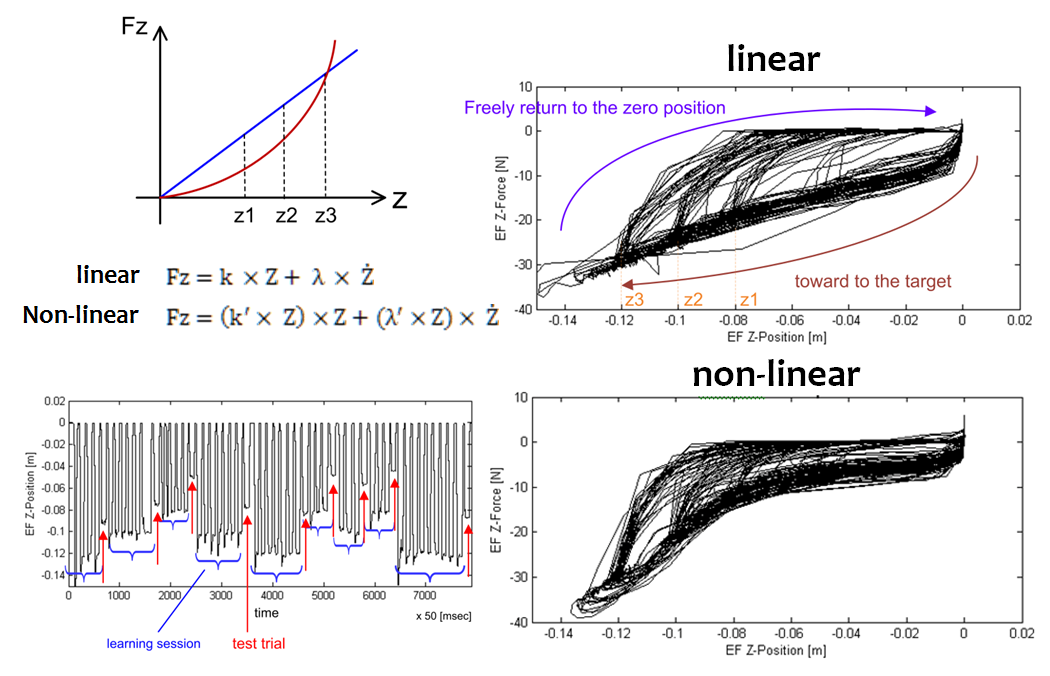
\includegraphics[width=.7\textwidth]{Chie/figs/Figure1.png}
  \caption{The experimental design of the pilot study and the movement profile of one subject as an example. A. a cartoon of linear and non-linear force. B. time vs. z position.
C. end effector z position vs. force (linear case). D. end-effector z position vs. force (non-linear case).}
  \label{expdesign}
\end{figure}

\textit{The main block consisted of two parts: Learning session and Test trial. In the Learning session, the target position was coloured circle (either z1, z2, z3, randomly assigned). Participants controlled the end-effector to reach the target from the start position within a certain time window. Participant received a feedback message when they did not reach the target in appropriate timing and retried it until three consecutive movements in success before the test trial. In the Test trial, participants moved the end-effector to the half position of the target. In this phase, no visual feedback was given to the participant in the relationship between the end-effector position and the target. One block consists of (Learning session + Test trial) x three positions (z1, z2, z3) x 3 times = 9 trials. Participants conducted three blocks; so, 27 test trials for each task “set the half-position” and “set the half-force” in total. The experiment was completed within approximately 60 minutes on average.}

Figure 2 shows the average positions and average force in the test trials across seven participants. In the half-position task, the graph indicate that all positions overshoot than the expected position for both linear and non-linear but the non-linear case was much better than the linear case. In the half-force task, the graph illustrate that the performance was overshoot than the expected force for linear case, in contrast, the performance was undershoot than the expected force for non-linear case.

\begin{figure}
	\centering
	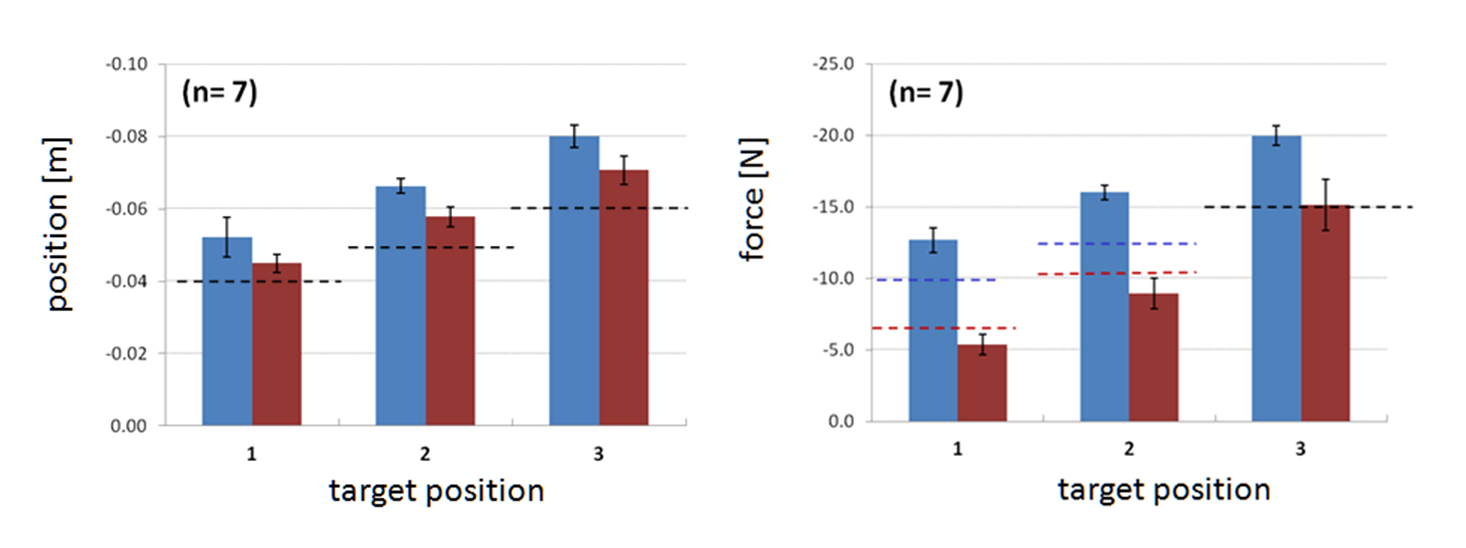
\includegraphics[width=.7\textwidth]{Chie/figs/Figure2.png}
	\caption{The results of one version of the pilot experiment. The bar charts represents the performance. Blue bars represent the linear condition and red bars represent the non-linear condition. A. “Set the half position” task. The dotted lines indicate the ideal position. B. “Set the half force” task. The dotted lines indicate the ideal force: blue for the linear force and red for the non-linear for the linear respectively.}
	\label{pilot}
\end{figure}
We have learned human performance specifically in relation to the tasks through the pilot experiments and according to the results briefly showed above, the important factors to be considered into the experimental design are listed up, and we conducted the main experiment by adapting some changes in the protocol. 

\subsection{Influence of Time} 
The results indicated higher overshoots in the linear case which can be an influence of the target time window used in the previous experiments. To avoid this influence, we removed the time-window to reach the target at the training session. This will allow the participants to reach the target with slow speed and will permit exploring the force dynamics within a certain period (it’s much longer than the previous time windows).

\subsection{Position Accuracy vs Velocity} 
Instead of the constraint of the speed to reach the target, participants were asked to reach the target position with certain accuracy at the training session; for example, within $\pm 5$mm. If it’s over or under the range (overshoot or undershoot) at the learning session, it would be judged as an error; then participants will be asked to repeat it until the position is as accurate as possible. The participants had to reach the target position most accurately for three times (non-consecutively).

\subsection{Force dynamics evaluation}
To evaluate the force dynamics in terms of position accuracy and velocity, the number of reachable target is reduced to one. Three targets without a stipulated time/velocity limitations will lead to longer trials, which might be exhaustive to perform.  Instead, we proposed evaluating with four different force dynamics with one reachable target position. The testing of half-position and half-force is still considered in all the four cases.

\subsection{Learning model}
A learning block is introduced at the beginning of each force dynamics evaluation, to provide more trials to explore and understand the movement performed. The lack of time or accuracy limitations will make the users to learn the movement completely and further understanding the human-learning performance for different forces.

\section{Learning Analyses}
Human learning model for compliant contact forces and specific reachable tasks are interesting in analysing and understanding the underlying reasons behind the human performance. 

The performance and learning ability of the human in specific visual guided tasks explains the human performance in dynamically compliant contacts \cite{ernst2002}. This learning model helps in understanding the human impedance behaviour which can further help in improving the robot performance. This also helps in identifying the human-robot interaction model to be developed and used in creating a human friendly robot. 

Humans perceive the applied force based on the input from the contact model and the compliance of the system \cite{pongrac2006}. To understand the influence of the human behaviour in different force model applications it is important to understand the impact of such forces and the learning model of the human interaction. The human force interaction model is also a subjective model depending on  each human subject’s ability and involvement in the interaction. Indeed, the interaction can be limited by defining a target position model to be reached and the velocity to be maintained while maintaining the target position.

This learning analysis helps in understanding the human-force perception or how humans perceive the different force dynamics, provided there is a position limitation. Further, it explains if they can differentiate (cognitively) the force models and their applied effort. This led us to further analyse how individual perception vary or if they can relate this force models to any activity for daily living scenario. Moreover, it is interesting to compare the human perception both verbally and cognitively to understand how the human perception model works. Including a simple questionnaire is another way to understand the human haptic force perception model, especially in relation to the forces applied in any daily activity \cite{van2014}. The questionnaire involves multiple real life scenarios which can explain the linear and non-linear forces.


\subsection*{Dynamic learning evaluation}
The dynamic learning metric evaluation is performed using the target position maintained with a constant velocity at the end of the goal position.

Metrics for dynamic learning analysis:
%
\begin{equation}
M=Z-Z_d +K* (\dot{Z}-\dot{Z_d})
\end{equation}
%
Z is the target position reached at the end of each trial and $\dot{Z} $ is the velocity maintained at the target position; $Z_d$  and $\dot{Z_d }$  are the desired goal position and velocity respectively. K is a constant value defined as function of the output sampling rate. The sampling rate function with the velocity parameter will explain the change in the target position adding some more windows to be more accurate.  The goal of this analysis is to observe the number of trials needed for each user to reach the target position as accurate as possible, provided the velocity is maintained at zero, at the end position.

The objective of this learning model is to understand the human perception and precision in reaching a specific target position. There was no time limitation to reach the target position, providing the users have enough chances/time to understand the different forces. 

\section{Methods}

\subsection{Apparatus and stimuli}
Similar to the initial pilot experiment, the current study employed a haptic device, Haptic Master (Moog, Inc.), which consisted of a large robotic rod with an end-effector. The device is controlled by a set of computer programmes to render robotic manipulandum for force feedback. We measured the end-effector movements controlled by human subjects and analysed the dynamic properties of the movements against the compliant force and the performance. The forces and the movements were constrained in vertical (Z) direction to the ground only.

We used the ready-made spring model in the Haptic API, where the compliant force formula was assigned to the device. The compliant force was rendered by sending parameters (i.e. spring stiffness and damping factor) in real-time depending on the end-effector position and the velocity (Figure 3).

%
\begin{figure}
	\centering
	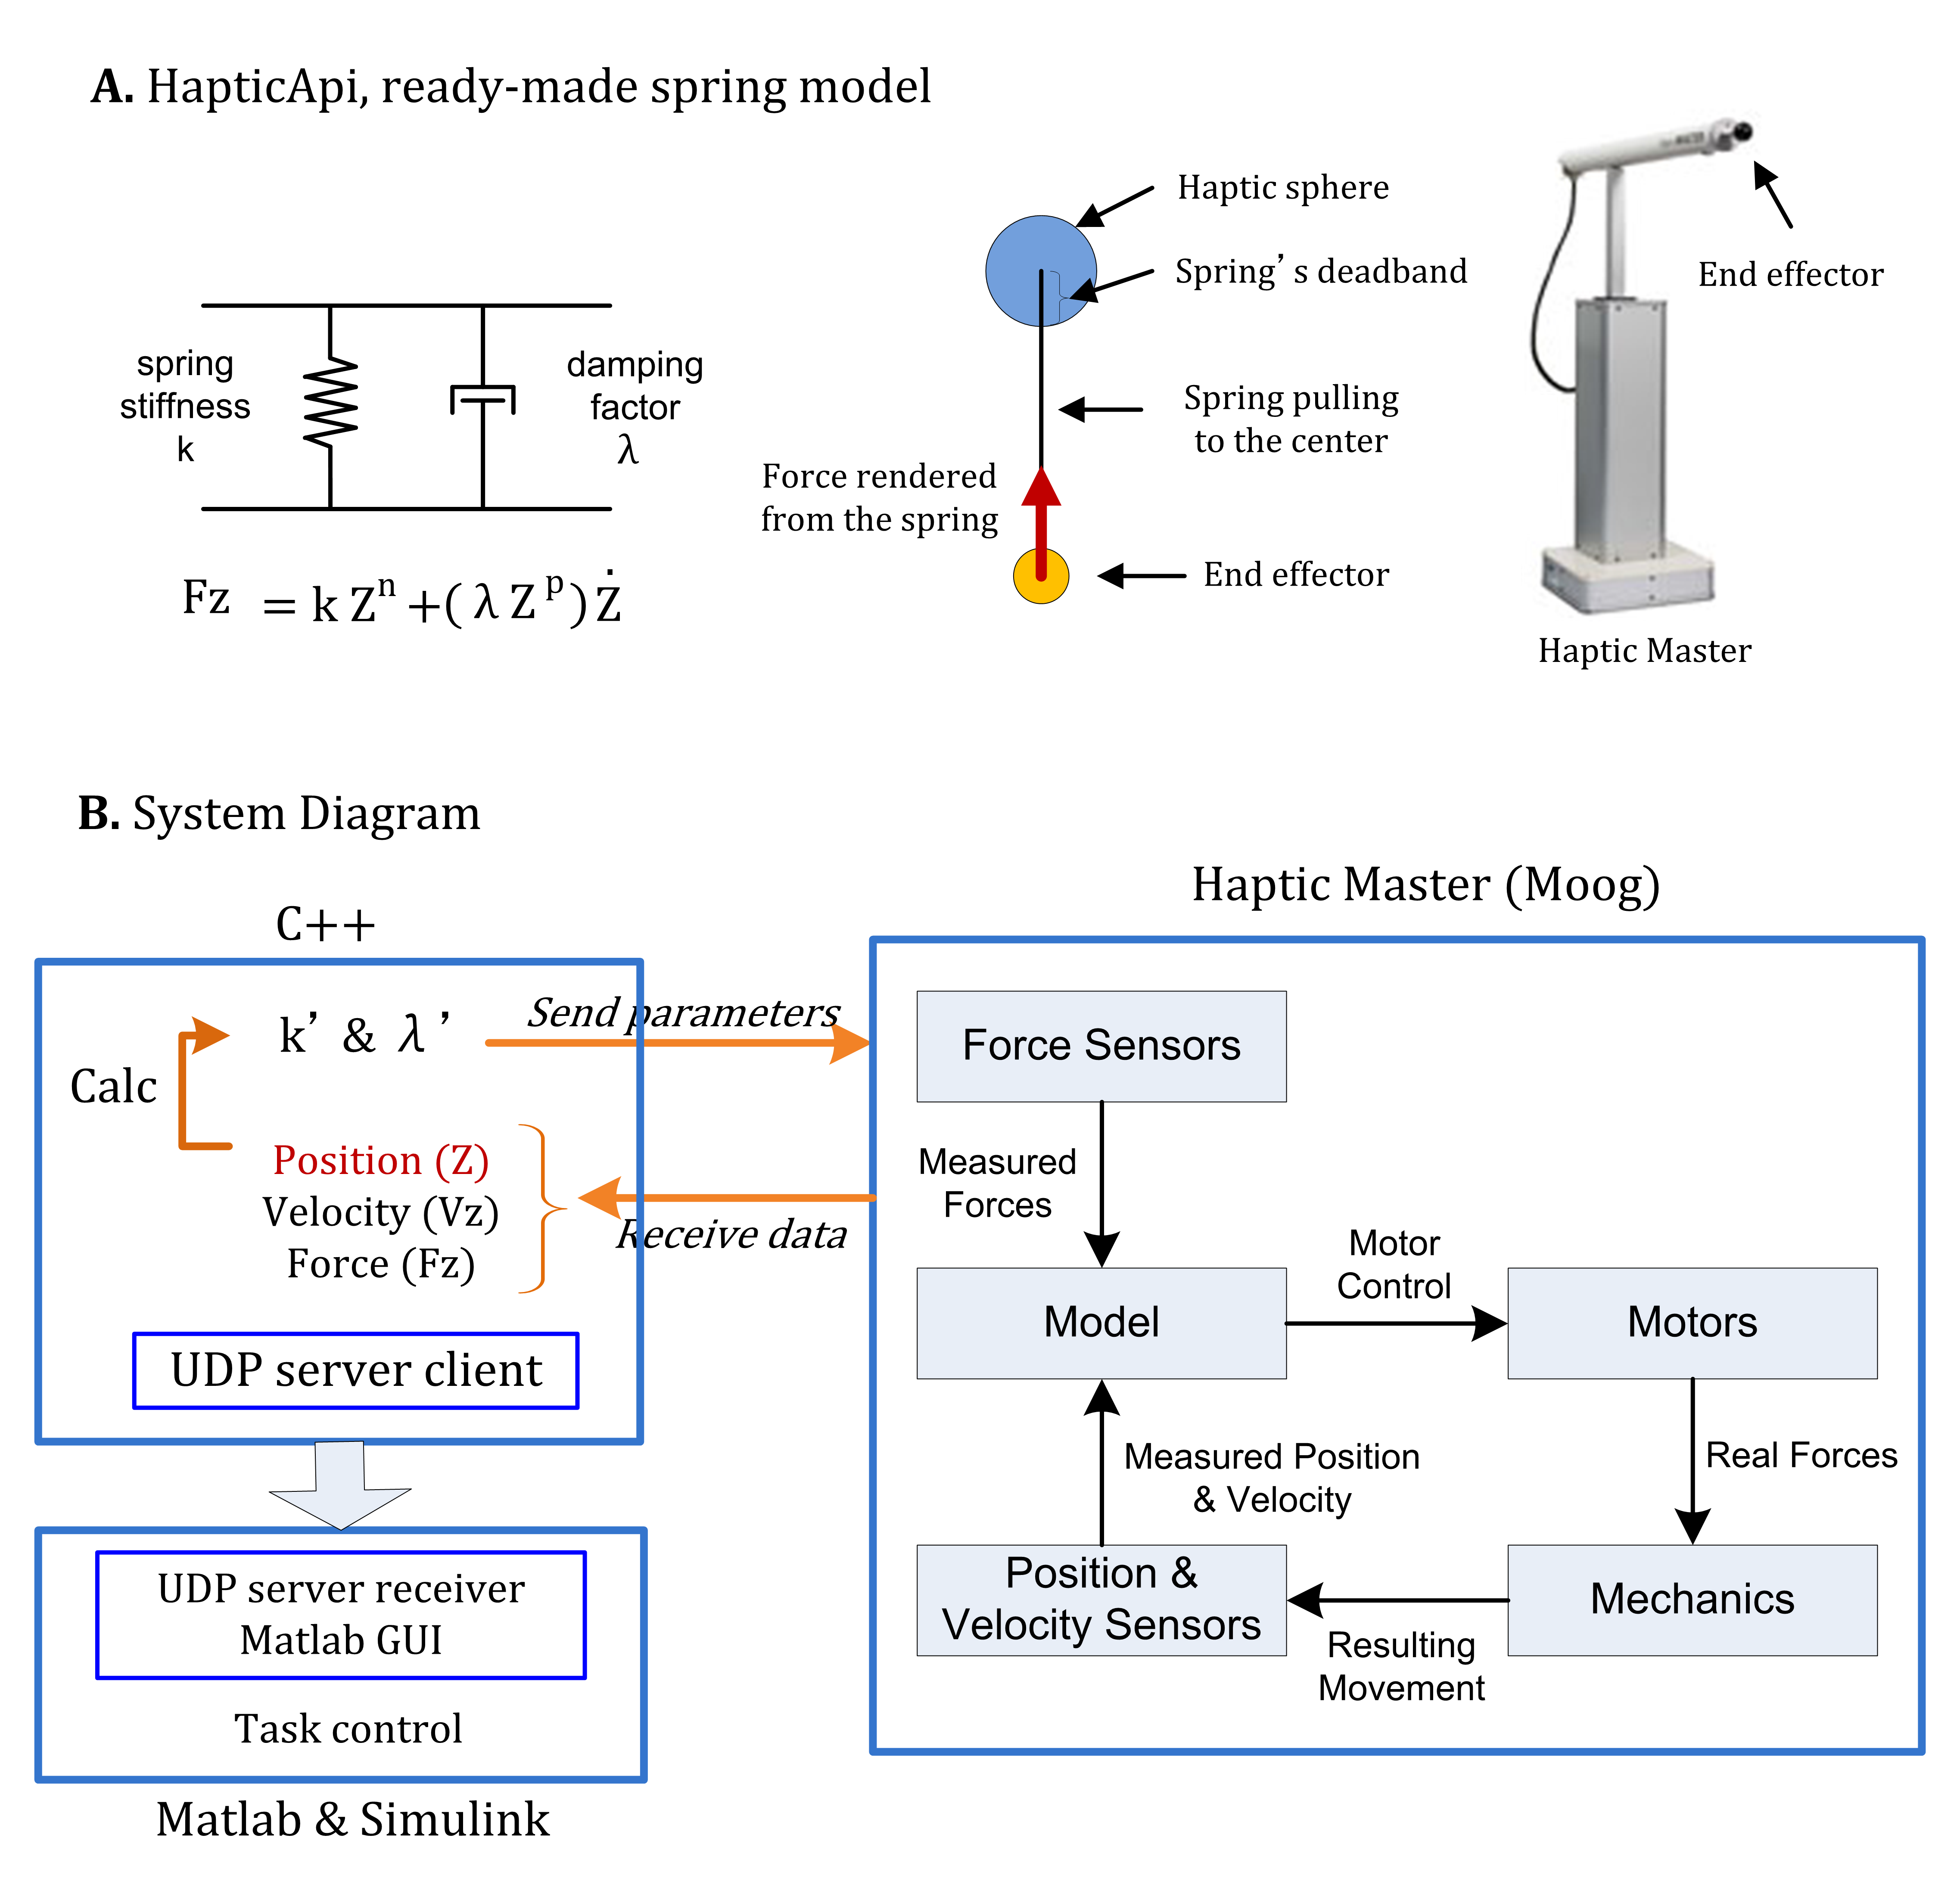
\includegraphics[width=.7\textwidth]{Chie/figs/Figure3.png}
	\caption{A. The ready-made spring model in the Haptic API. B. A block diagram of the compliant force control. The force is rendering based on the end-effector position and the velocity with parameters (spring stiffness and damping factors) in the real time.}
	\label{modelling}
\end{figure}

\subsection{Experimental Design}

\subsubsection{Different force dynamics}
In general, spring-damper force ($\BF$) is formulated by the position and the
velocity with parameters: spring stiffness ($k$) and spring damping factor
($\lambda$).  Here, it is simplified for one direction ($\BZ$).
%
\begin{equation}
\BF = k \BZ^n + (\lambda \BZ^p) \dot{\BZ} \, .
\end{equation}
%
We generated four different compliant forces (two linear and two non-linear cases) by changing the stiffness k values (see Figure 4 and Table 1). The k value is maintained constant in linear case and position dependent in case of non-linear forces. In Figure 4, the linear cases are [1] and [4], and the non-linear cases are [2] quadratic and [3] concave, respectively.
\begin{figure}
	\centering
	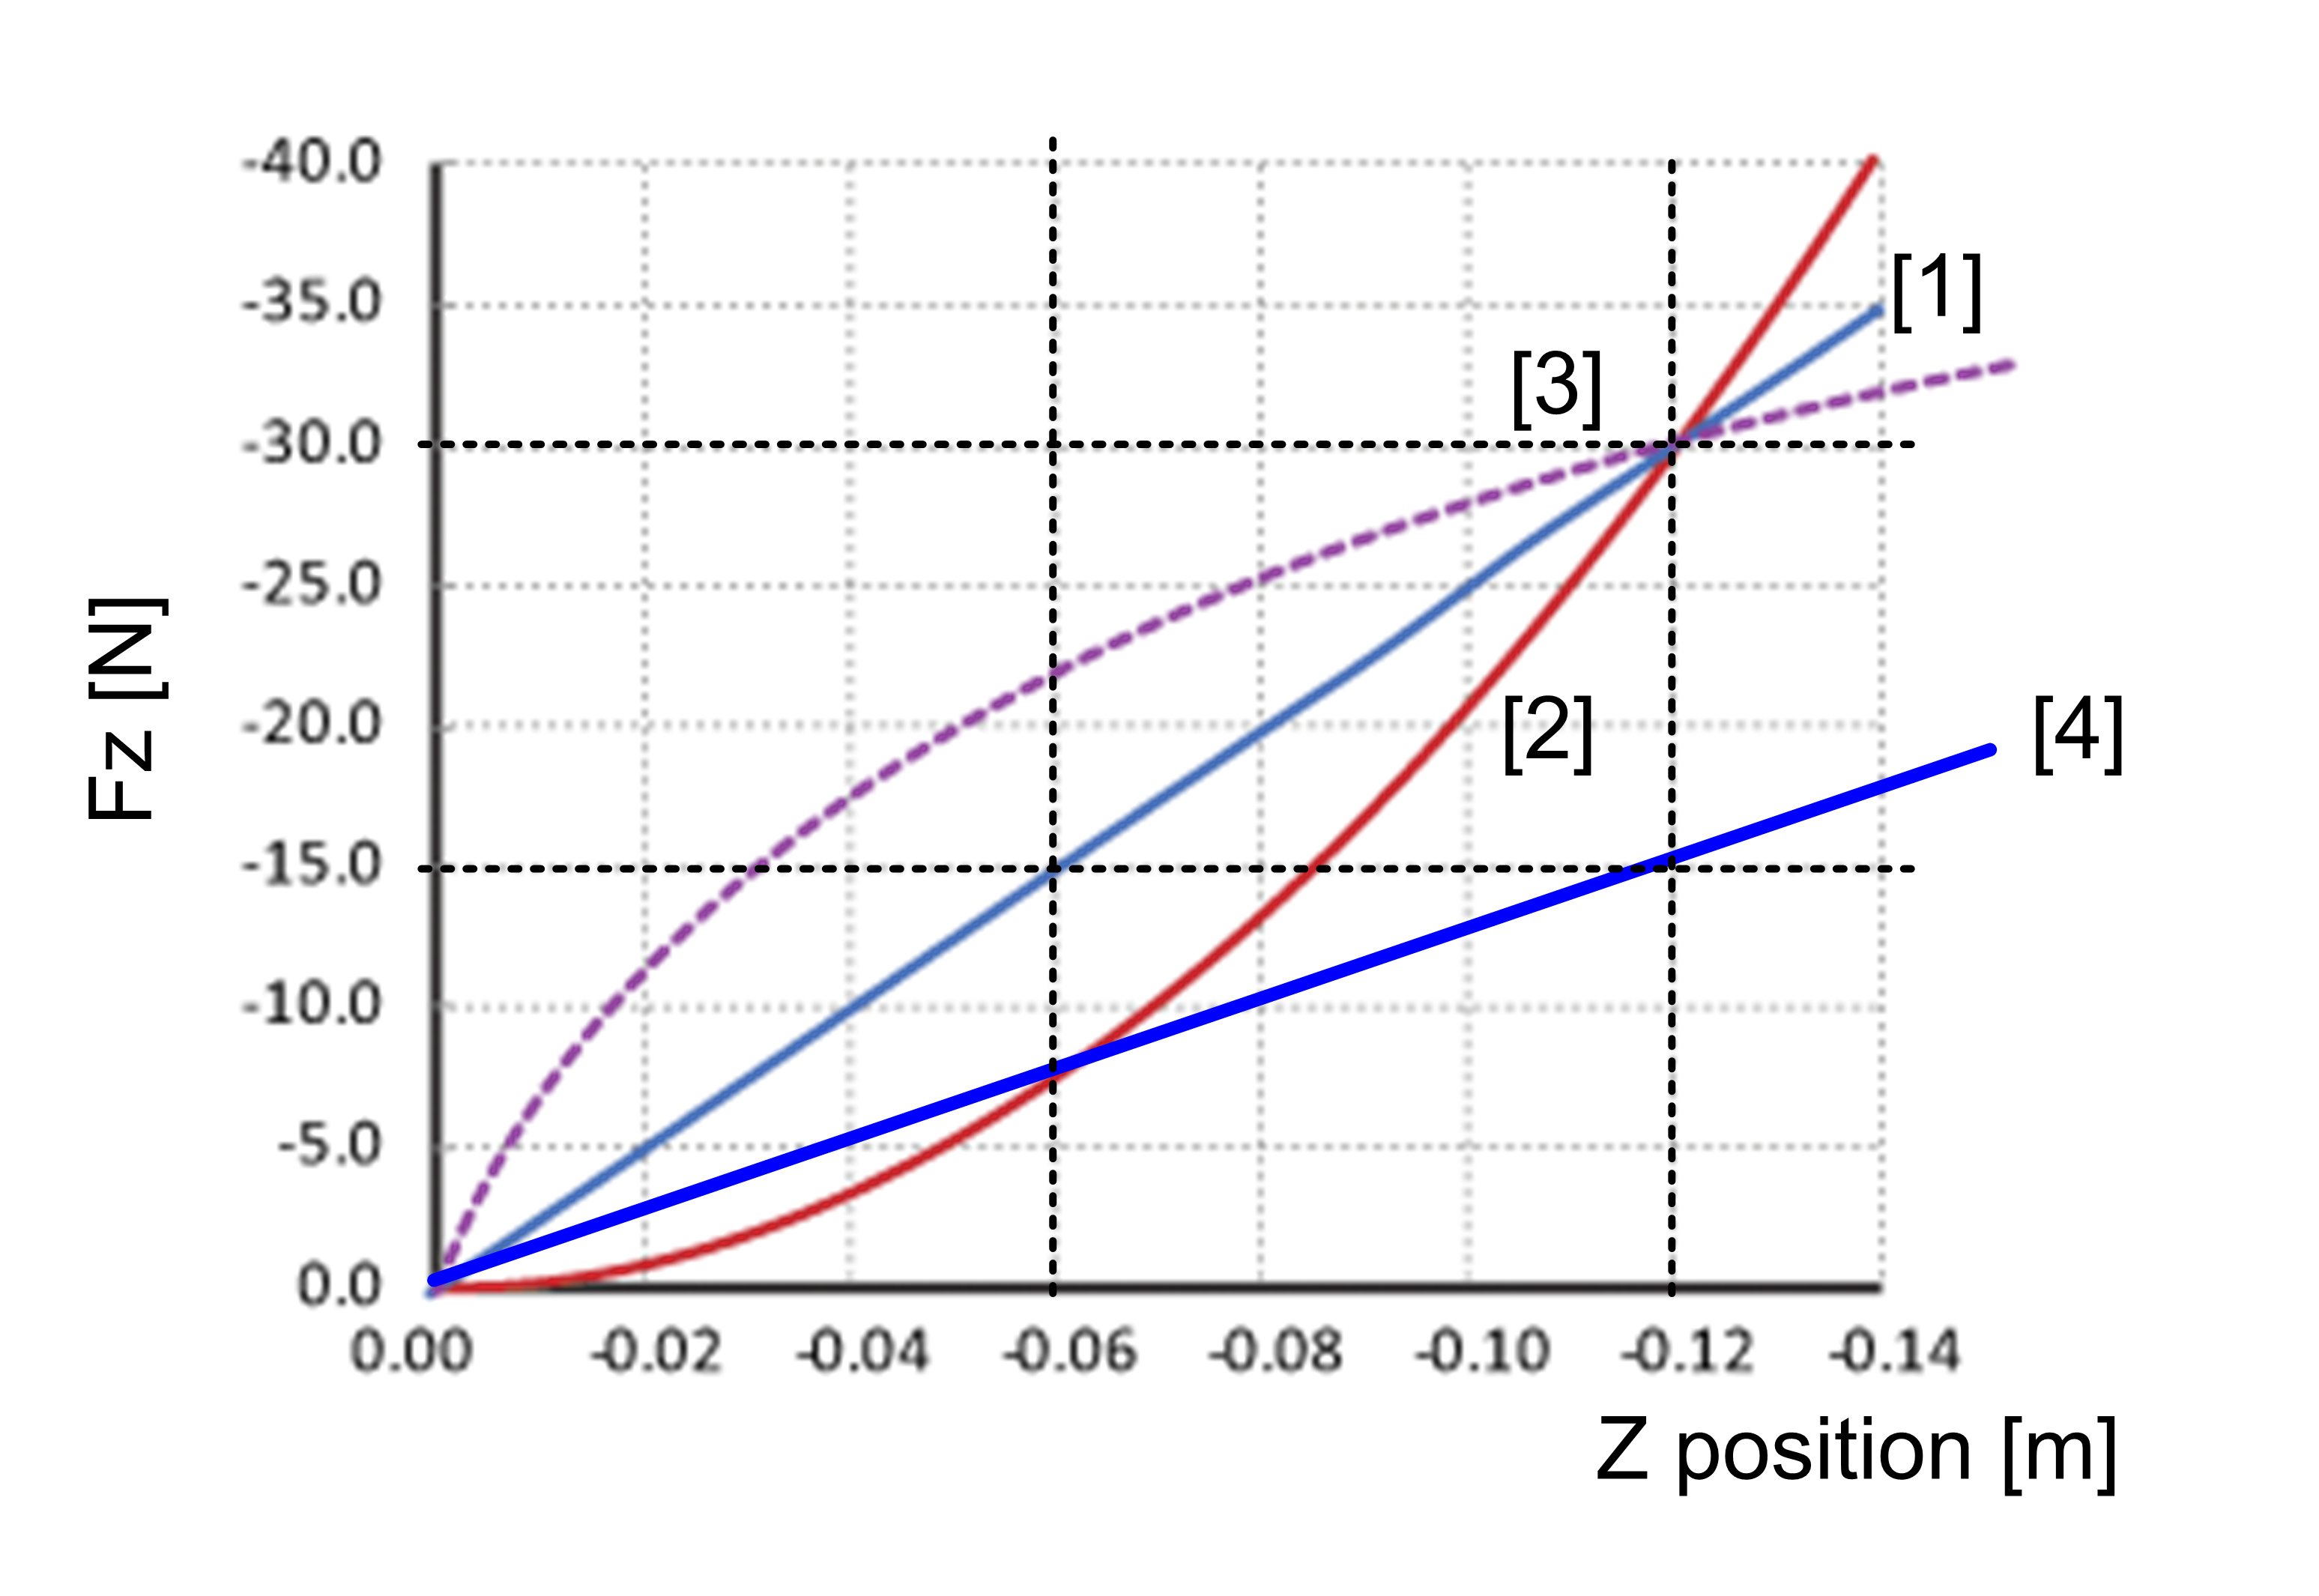
\includegraphics[width=.7\textwidth]{Chie/figs/Figure4.png}
	\caption{Four different force dynamics are applied. [1] Linear, [2] Non-linear (quadratic), [3] Non-linear (concave), and [4] Half-linear. The [1],[2],[3] are the same force at the end position (e.g., z=-0.12), and [2] and [4] are the same force at the half position  (e.g., z=-0.06).}
	\label{forcedyn}
\end{figure}

\begin{figure}
	\centering
	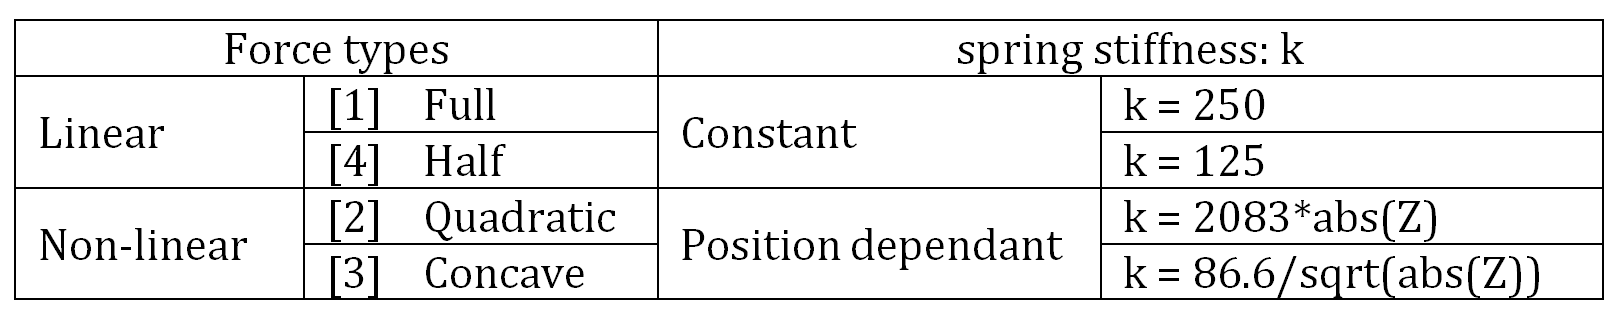
\includegraphics[width=.7\textwidth]{Chie/figs/Table1.png}
	\caption{Table 1. The four different forces are rendered by changing the spring stiffness. See the parameters in the table.}
	\label{Table1}
\end{figure}

\subsubsection{Questionnaires}
The questionnaire (Q1 and Q2) we introduced to this experiment can be seen in Table 2. It is interesting to compare the human perception both verbally and cognitively to understand how the human perception model works. A simple questionnaire to rate the effort to deal with the applied force (Q1) is a way to understand the human haptic force perception model \cite{tan1994}, compared with the individual physical performances. Moreover, it is beneficial to examine the force perception in relation to the forces applied any daily activities (Q2). The questionnaire involves multiple real life scenarios which can be explained by the linear and non-linear forces. Individual subjective responses to this questionnaire would also help to understand human physical performance and also bridge the relationship between human motor control against the force and the subjective force perception.

\begin{table}
\begin{center}
	\caption{Questions and responses. This questionnaire was introduced to examine human haptic force perception after a certain exposure to the repetitive movements against a specific compliant force. All questions were repeated at the end of each session.}
\resizebox{0.9\textwidth}{!}{
	\begin{tabular}{c|c}
		Questions & Responses \\
		\\Q1.Rate the applied force in terms of effort.
		&1. Extremely Low\\
		&2. Low\\
		&3. Moderate\\
		&4. High\\
		&5. Very High \\
		\hline
		\\Q2.	How do you relate this force with a common day-to-day activity?
		& a.	 Pushing a cushion\\
		& b.	 Pushing a revolving door\\
		& c.	 Pushing a box on a plane surface\\
		& d.	 Pushing a hinged door\\
		&  e.	 Pushing a box on an inclined surface\\
		\hline
	\end{tabular}}
\end{center}
\end{table}

\subsection{Experimental Protocol/Procedure}

\subsubsection{Protocol}
Based on the pilot experiments conducted and the in-depth analysis of the result, a detailed experimental protocol was designed as illustrated in Figure 5. Initially, a Practice Session was introduced using only the half-linear force to learn the complete task. Following the practice session, Three different force sessions (linear, quadratic, and concave) were “pseudo-randomly” assigned. The random order aimed to minimise the order effects on the performance.
\begin{figure}
	\centering
	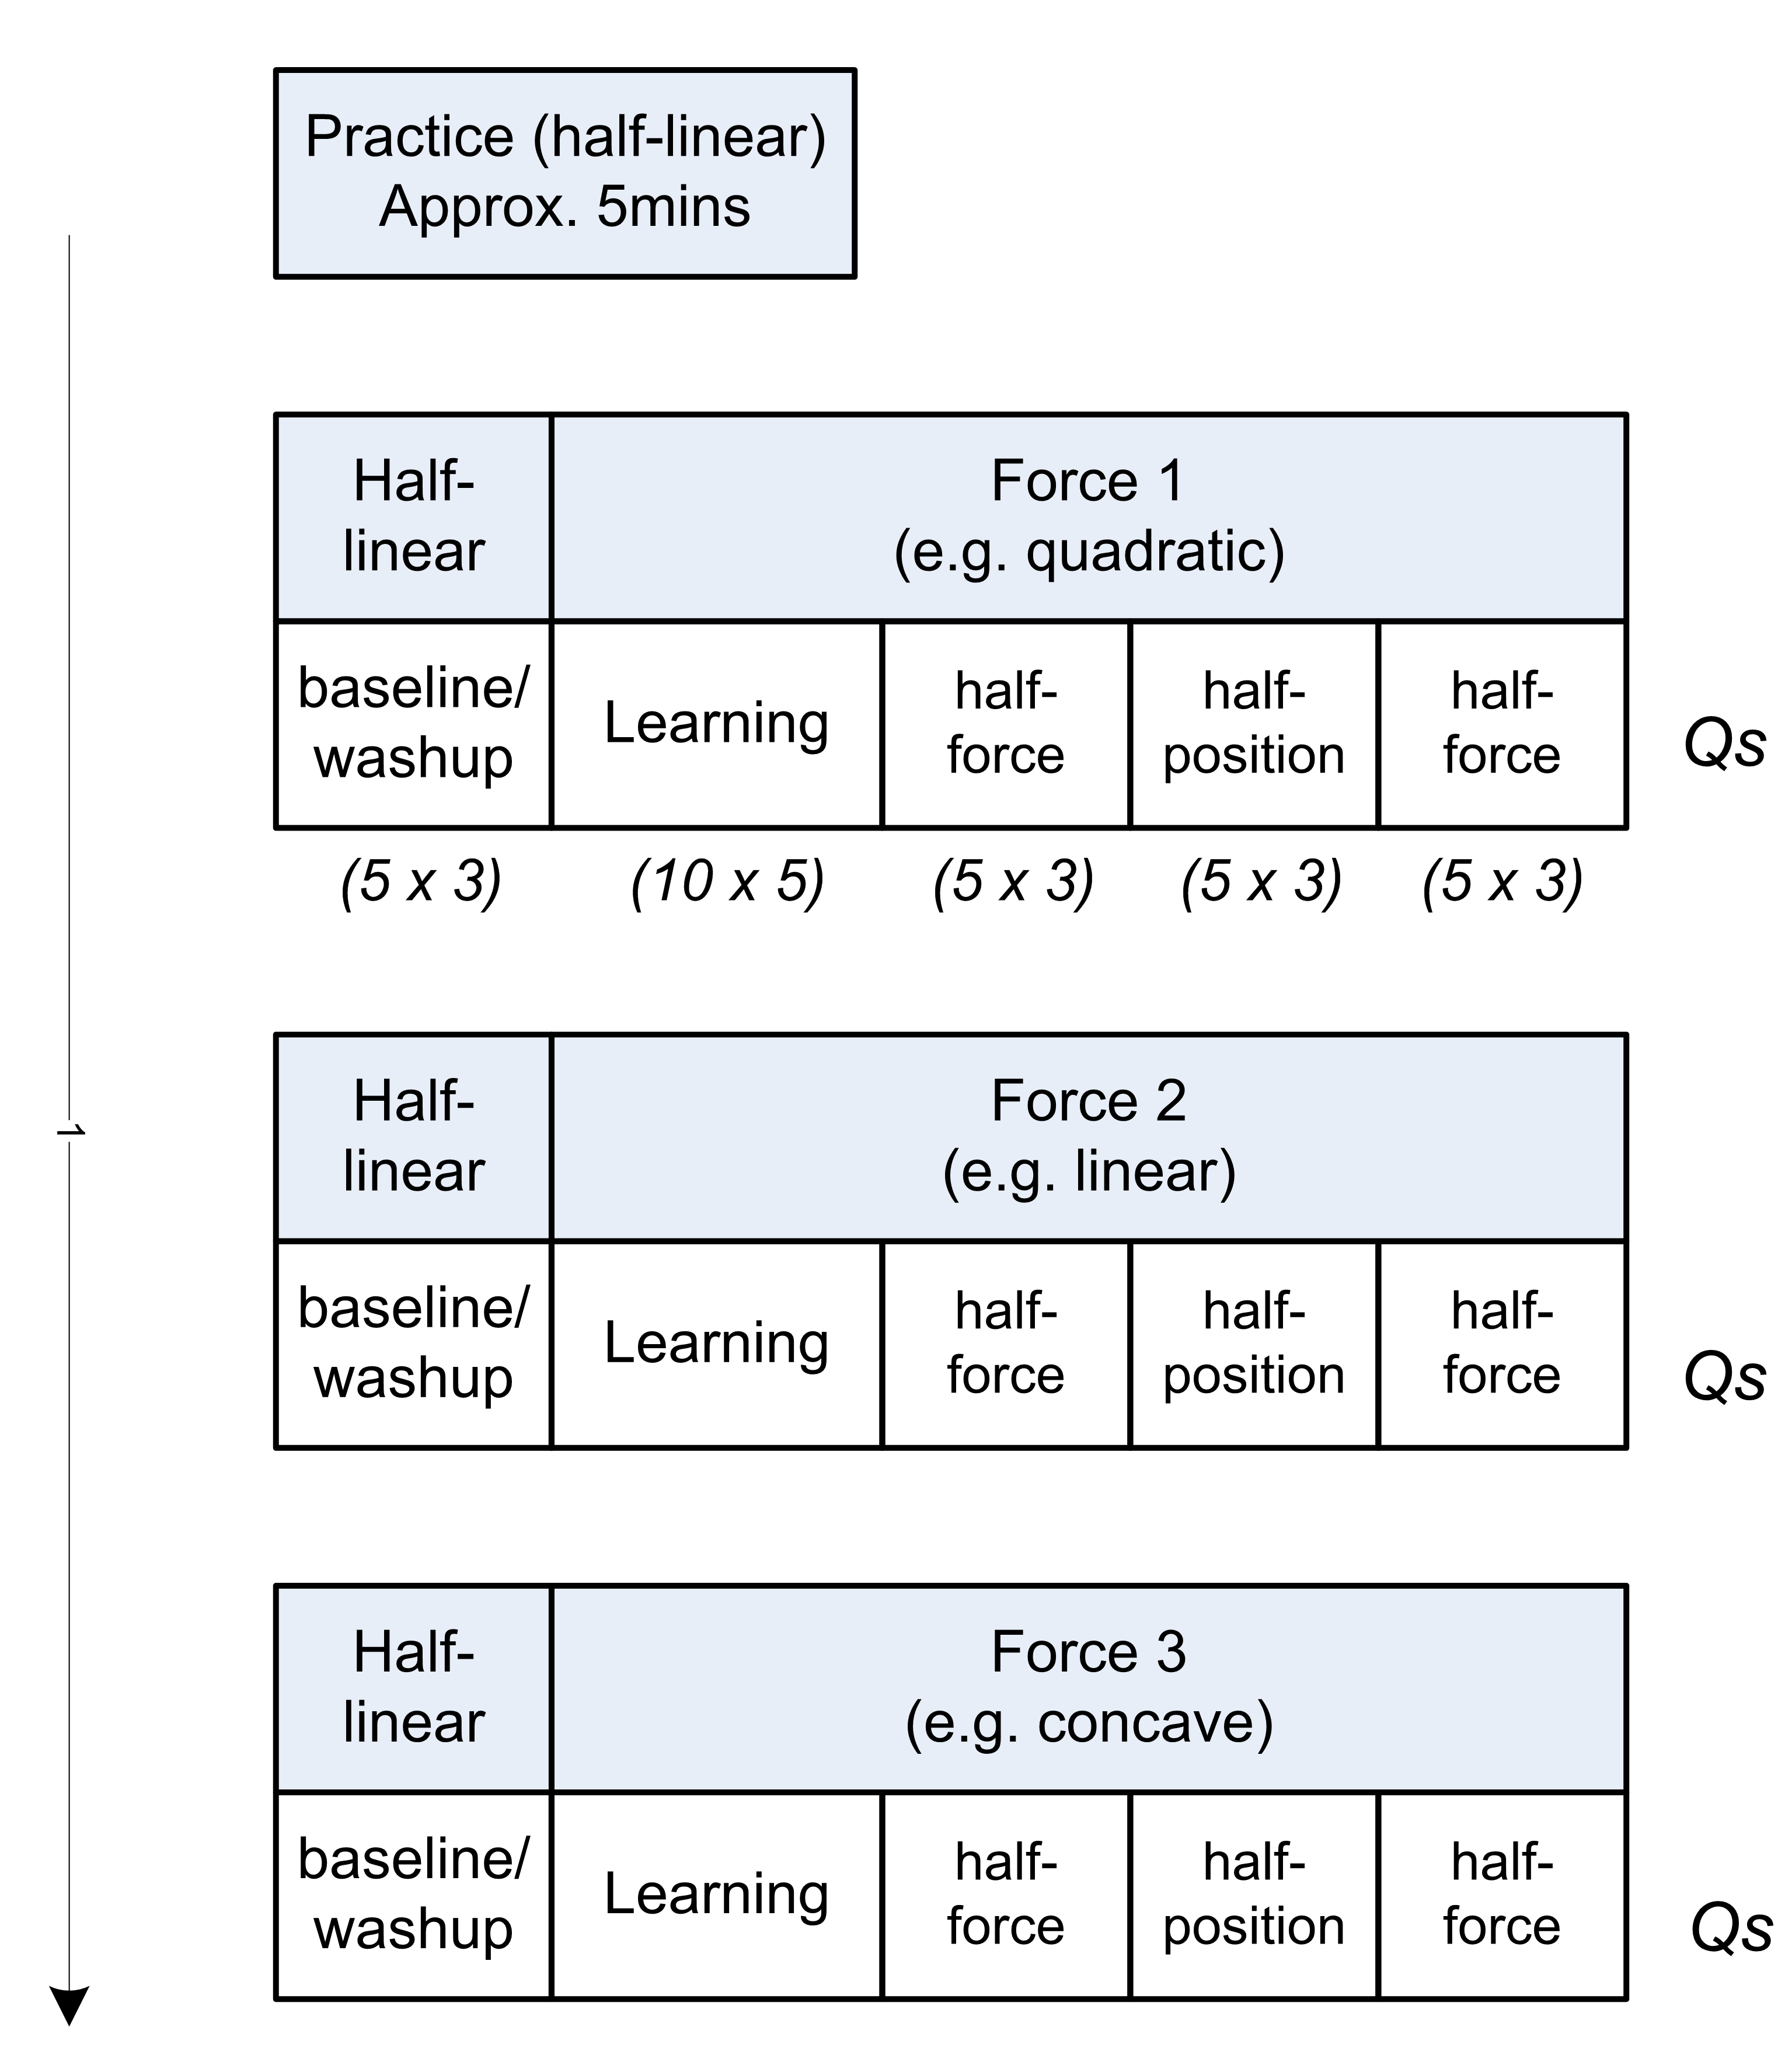
\includegraphics[width=.7\textwidth]{Chie/figs/Figure5.png}
	\caption{Experimental protocol. Approx. 5 mins practice session followed by three sessions with different (one linear and two non-linear) forces. Each session started with baseline/wash-up and learning blocks and then three test blocks. More details can be seen at the main text.}
	\label{protocol}
\end{figure}
Each session consisted of a series of five blocks (baseline/wash-up, learning, half-force, half-position, and then half-force). In all the blocks, there were a certain number of test trials. The test trials probed whether participants could appropriately produce either half-force or half-position of that they previously learned through their repetitive movements to reach the target.

-	The “half-linear” force block was set at the beginning of each force session as a baseline/wash-up. “The test trial asked a participant to set the force of the target previously learned” after five repetitive movements to reach the target position.
-	In the “learning” block, there were ten test trials: “Set the force of the target previously learned” after five repetitive movements to reach the target position.
-	In the “half-position” block, there were five test trials: “Set the half-position of the target previously learned” after three repetitive movements to reach the target position.
-	In the “half-force” block, there were five test trials: “Set the half-force of the target previously learned” after three repetitive movements to reach the target position.
-	The half-force block was conducted twice; so the total was 10 test trials.

After the completion of each session, a participant took a break and was asked to answer a few questions aiming to assess subjective perception to the force he/she experienced.

\subsubsection{Procedure}
At the beginning of the experiment, all participants received the instruction from the experimenters. After understanding the task well, a participant stood in front of the haptic device and grasped the end-effector.

The “Home” position, where was the centre of the end effector is z = 0 at the workspace, was 110 cm from the ground. The spring position was set at z = 0. In this study, the rod movements were restricted in the vertical direction only. The target positions were set at z = 120 mm.

The visual information about the task was provided at the computer display to human subjects.
The computer screen was located in front of human subjects; where the centre of the screen was align to the centre of the robotic rod. The screen was approximately 1.60m away from the participants’ standpoint. Height from ground- approx.162cm, screen display size 531.36mm (Ht) x 298.89mm (W). The screen displayed the target position and the end-effector position in real-time, excluding the test trials (Figure 6). 
%
\begin{figure}
	\centering
	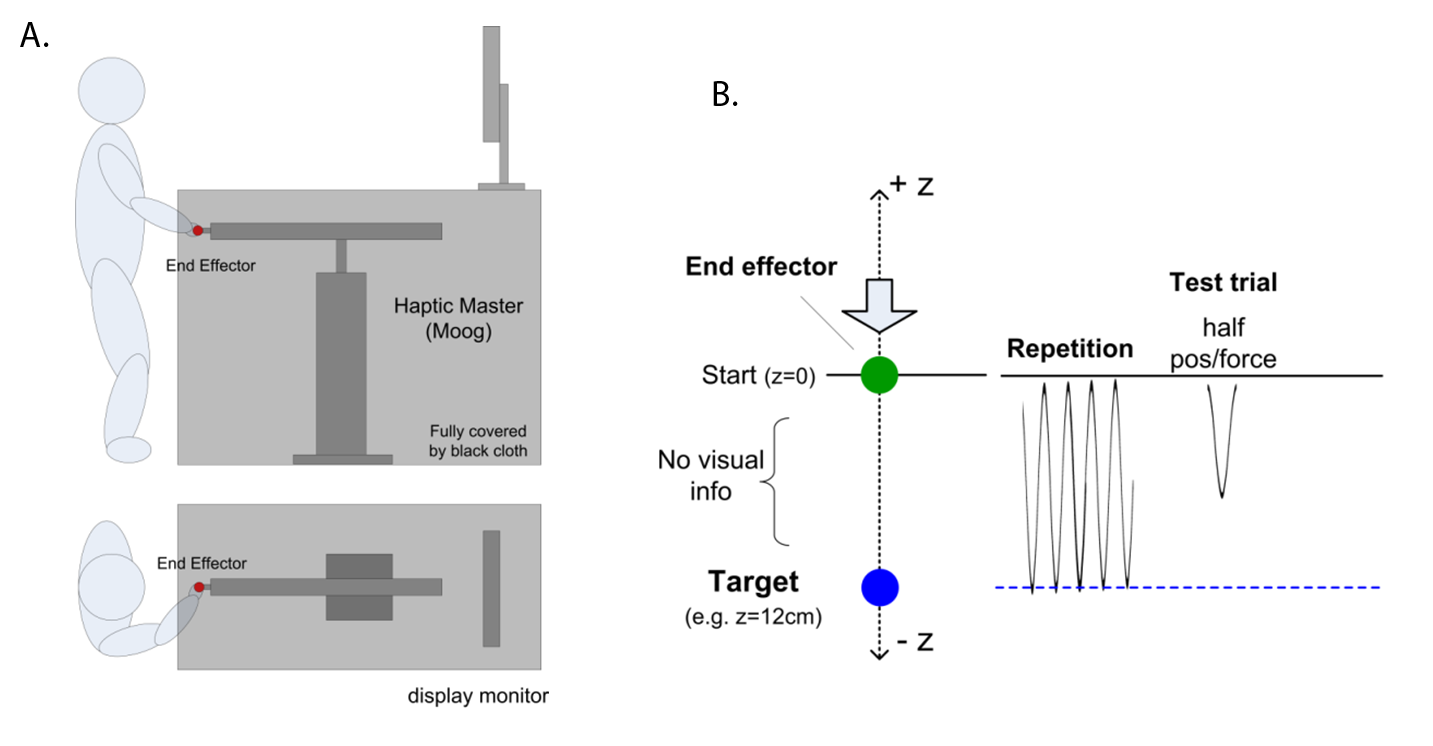
\includegraphics[width=0.95\linewidth]{Chie/figs/Figure6.png}
	\caption{A. A cartoon of an experimental setting. B. The explanation of the experiment. The end-effector and the target positions were visually indicated on the computer screen during the repetitive period, but there were no visual info at the test trial. .}
	\label{settingHM}
\end{figure}

Based on the experimental protocol as described above, all participants begin with the practice session followed by the main sessions. They were required to make repetitive movements against the compliant force generated by the haptic device to learn kinetic principle. Participants pushed the end-effector to reach the target position, and then released the end-effector to allow it to freely return to the initial position (z = 0). The end-effector movements were monitored by the computer systems and the visual information was provided on the screen, excluding between the start position and the target position (See Figure 6 B.) The target zone was visually defined by a coloured circle. The colour was controlled by the Matlab/Simulink computer programme and changed depending on the condition, aiming to inform the condition to participants. 

In the repetitive period, participants were asked to reach the target position$ (z = -0.12 m)$ within a certain time window $(0.6\pm 0.2s)$ as accurate as possible. The timer started when the end-effector moved from the initial position and stopped when the end-effecter position crossed the target position.  Participants received the feedback message for the each movement on the display:  “too fast” when $< 0.4 s$, “good timing” $0.4s \leq t \leq 0.8 s$, and “too slow” when $t > 0.8 s$. They were also requested to set the end-effector within the target zone as accurate as possible and to keep it staying there for approx. 1 sec, ideally maintaining it with zero velocity.

In the test trial, in the “practice” and “learning” blocks, participants were asked to set the end-effector at the same feeling of the force at the target previously learned after the repetitive movements. In the “half-force” block and the “half-position” block, the test trials asked participant to set the end-effector at the same feeling of the half-force or the half-position, respectively. They were requested to keep the end-effector there with no visual feedback and to maintain it with zero velocity for approx. 2sec.

In order to help the participants concentrate in the force analysis and the compliance, an alpha noise was introduced to the users. The participants had headphones on which also helped in removing the external or any environmental disturbances and to concentrate on the experiments.

\section{Results and Discussion}
\subsection{Participants}
Eighteen subjects (age range: 18 ~ 41,) took part in the experiment (12 female, 18-41 years old, mean age: $20.4 +/- 5.2 (SD)$, mean height: $169.1 cm +/- 8.8 (SD)$, 14 right-handed). All the participants had normal or corrected to normal vision, and no known motor deficits and/or any limb injuries by self-reported. The study was approved by the Research Ethics Committee, University of Birmingham, and all procedures were in accordance with the Declaration of Helsinki. Participants were recruited via the University Research Participant Scheme – SONA System . Subjects gave informed consent to participate, but were naïve to the purpose of the experiment. They also have no prior knowledge about the system or the force models chosen.

\subsection{Responses to the three different force dynamics in the test trials}
The sensorimotor physical properties (e.g. distance, velocity, and force) were collected through sensors, mounted at the end effector, while the human subjects were controlling their movement under different force dynamics were applied. The dynamic properties of the point-to-point movements were measured: the end-effector’s position (z), the velocity $\dot{z}$, and the force (Fz) across the time. These were recorded by the 20Hz sampling rate. We read-out the data (position and force) at the test trials in the “half-position” task and “half-force” task and analysed the differences between the three different force conditions. Figure 7 shows one of the participants performance as an example.
%
\begin{figure}
	\centering
	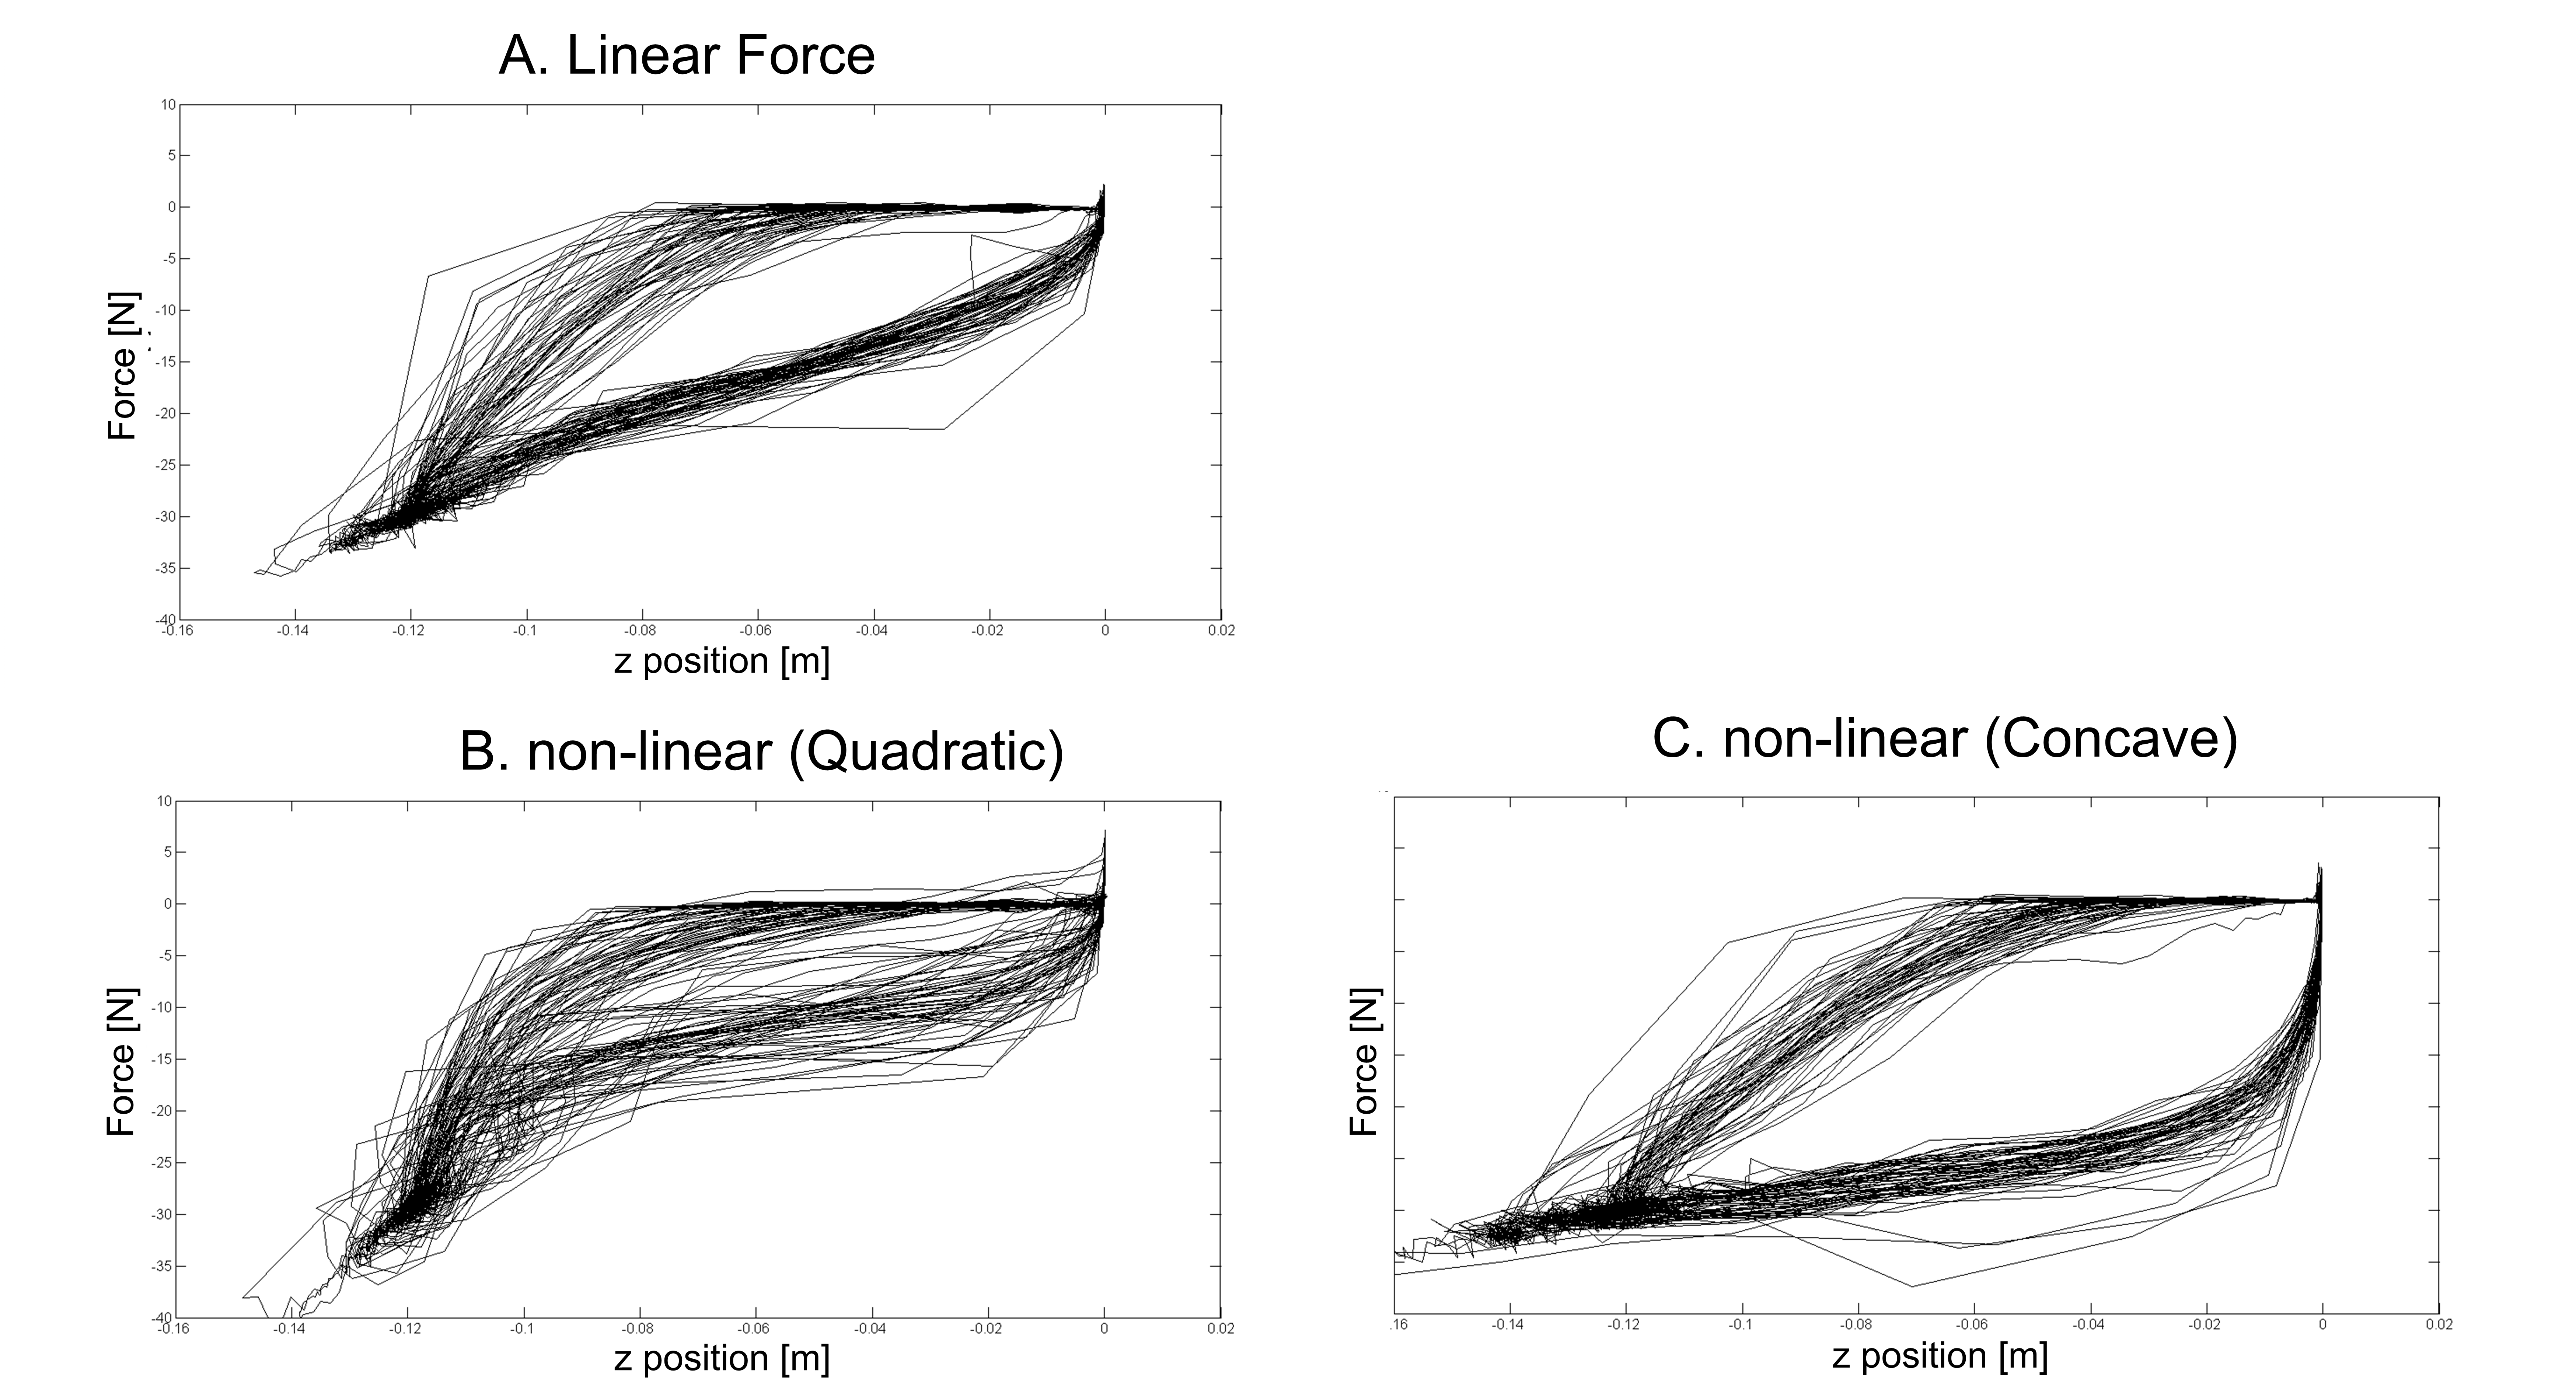
\includegraphics[width=0.7\textwidth]{Chie/figs/Figure7.png}
	\caption{An example of one participant’s movement profile. The three graphs represent the properties of the movements (position vs force) under three different conditions. A. linear, B. quadratic, and C. concave.}
	\label{modelling}
\end{figure}
\subsubsection{“Set the half position” performance}
Figure 8 shows the averaged performance across 5 test trials in the “half-position” task. In this task, participants kept the end-effector at the similar position which they felt as the half-position in the previous repetitive movements. Therefore, we evaluate how they accurately move the end-effector compared with the “target” half position.
%
\begin{figure}
	\centering
	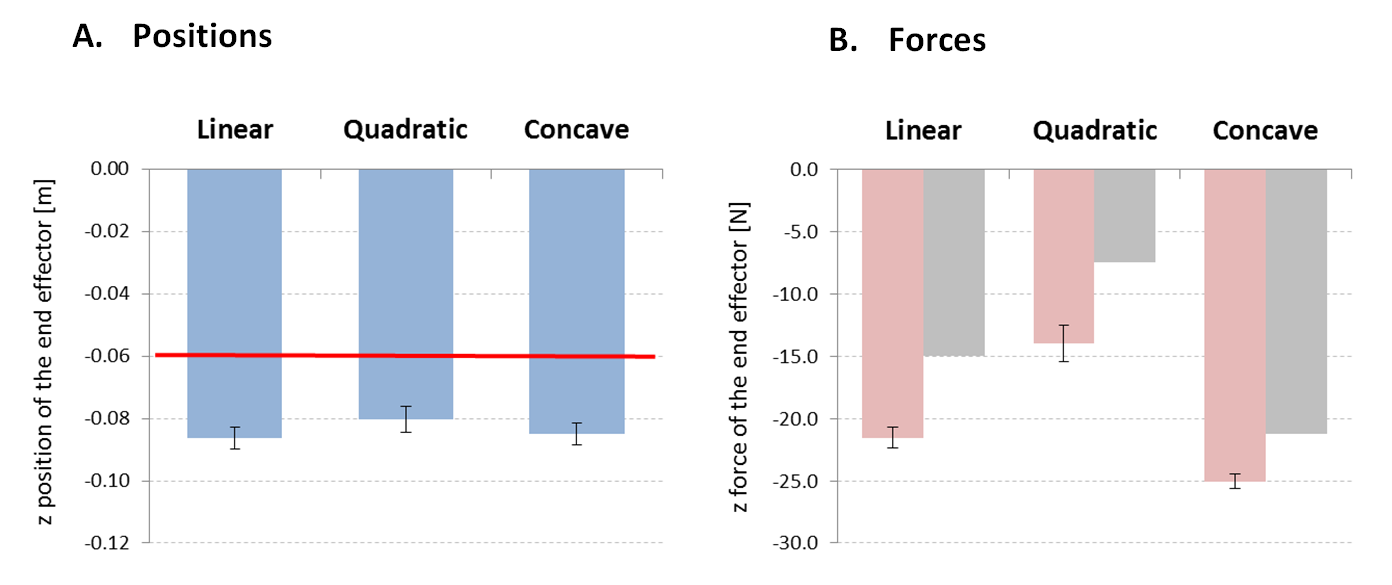
\includegraphics[width=0.7\textwidth]{Chie/figs/Figure8.png}
	\caption{The end-effector position and force at the test trial, averaged across 18 participants. 
		A. the positions for three different force conditions, compared with the red line representing the ideal position z = -0.06 [m]. B. the force for three different conditions, compared with the grey bars representing the “target” force (see Figure 4).}
	\label{testrial}
\end{figure}
According to the Figure 8A, an overshoot  from the target position $(z = -0.06 m)$ is observed for all the three conditions. This overshoot can be considered as the effect of the deprivation of visual-feedback in the test trials because the same performance was observed at the wash-up/baseline and learning blocks.

There were no significant position differences between three force conditions. A statistical analysis supports this. Mauchly’s test of Sphericity indicated that the assumption of sphericity had been violated, $\chi^2 (2) = 9.429, p = .009 < .05, $ therefore degrees of freedom were corrected using Greenhouse-Geisser estimates of sphericity $(\epsilon = .69)$. The results show that there were no significant differences on position perceptions under different force dynamics was applied, $F(1.384, 23.524) = 1.501, p = .240$.

\subsubsection{“Set the half force” performance}
Figure 9 shows the averaged performance across 10 test trials in the “half-force” task. In this task, participants kept the end-effector at the similar force as much as possible which they felt as the half-force in the previous repetitive movements. Therefore, we evaluate how they accurately move the end-effector compared with the “target” half force. 
%
\begin{figure}
	\centering
	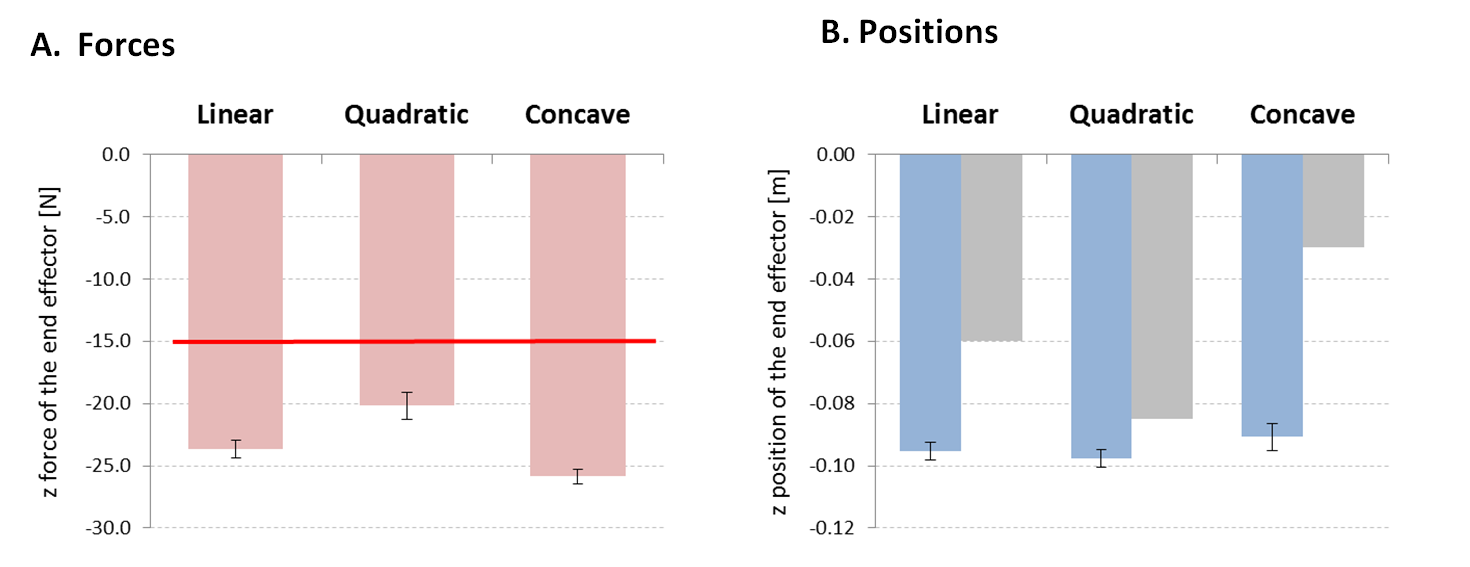
\includegraphics[width=.7\textwidth]{Chie/figs/Figure9.png}
	\caption{The end-effector force and positions at the test trial, averaged across 18 participants. 
		A. the forces for three different force conditions, compared with the red line representing the targeted force Fz = -15 [N].  B. the positions for three different conditions, compared with the grey bars representing the “targeted” force (see Figure 4).}
	\label{half-force}
\end{figure}
According to the Figure 9A, overshoot in forces  from the target force (Fz = -15.0 N) was also observed for  all the conditions. This overshoot also can be considered as the effect of the deprivation of visual-feedback with the same reasons as discussed above at the position task.

Figure 9A shows that there were significant differences between the three force conditions. Further statistical analyses were made. Mauchly’s test of Sphericity indicated that the assumption of sphericity had been violated, $\chi^2 (2) = 8.221, p = .016 < .05$, therefore degrees of freedom were corrected using Greenhouse-Geisser estimates of sphericity $(\epsilon = .71)$. The results show that there were significant performance differences in the half-force task under different force dynamics, $F(1.427, 24.255) = 27.165, p = .000$.

\subsubsection{Work of a force analyses}
The read-out positions and forces, as analysed above, might not well represent the influence of the force dynamics on the performance because of the pinpoint values. Here, we consider the influence by the exposure of the force dynamics for the movements and tried to conduct further temporal analyses.
%
\begin{figure}
	\centering
	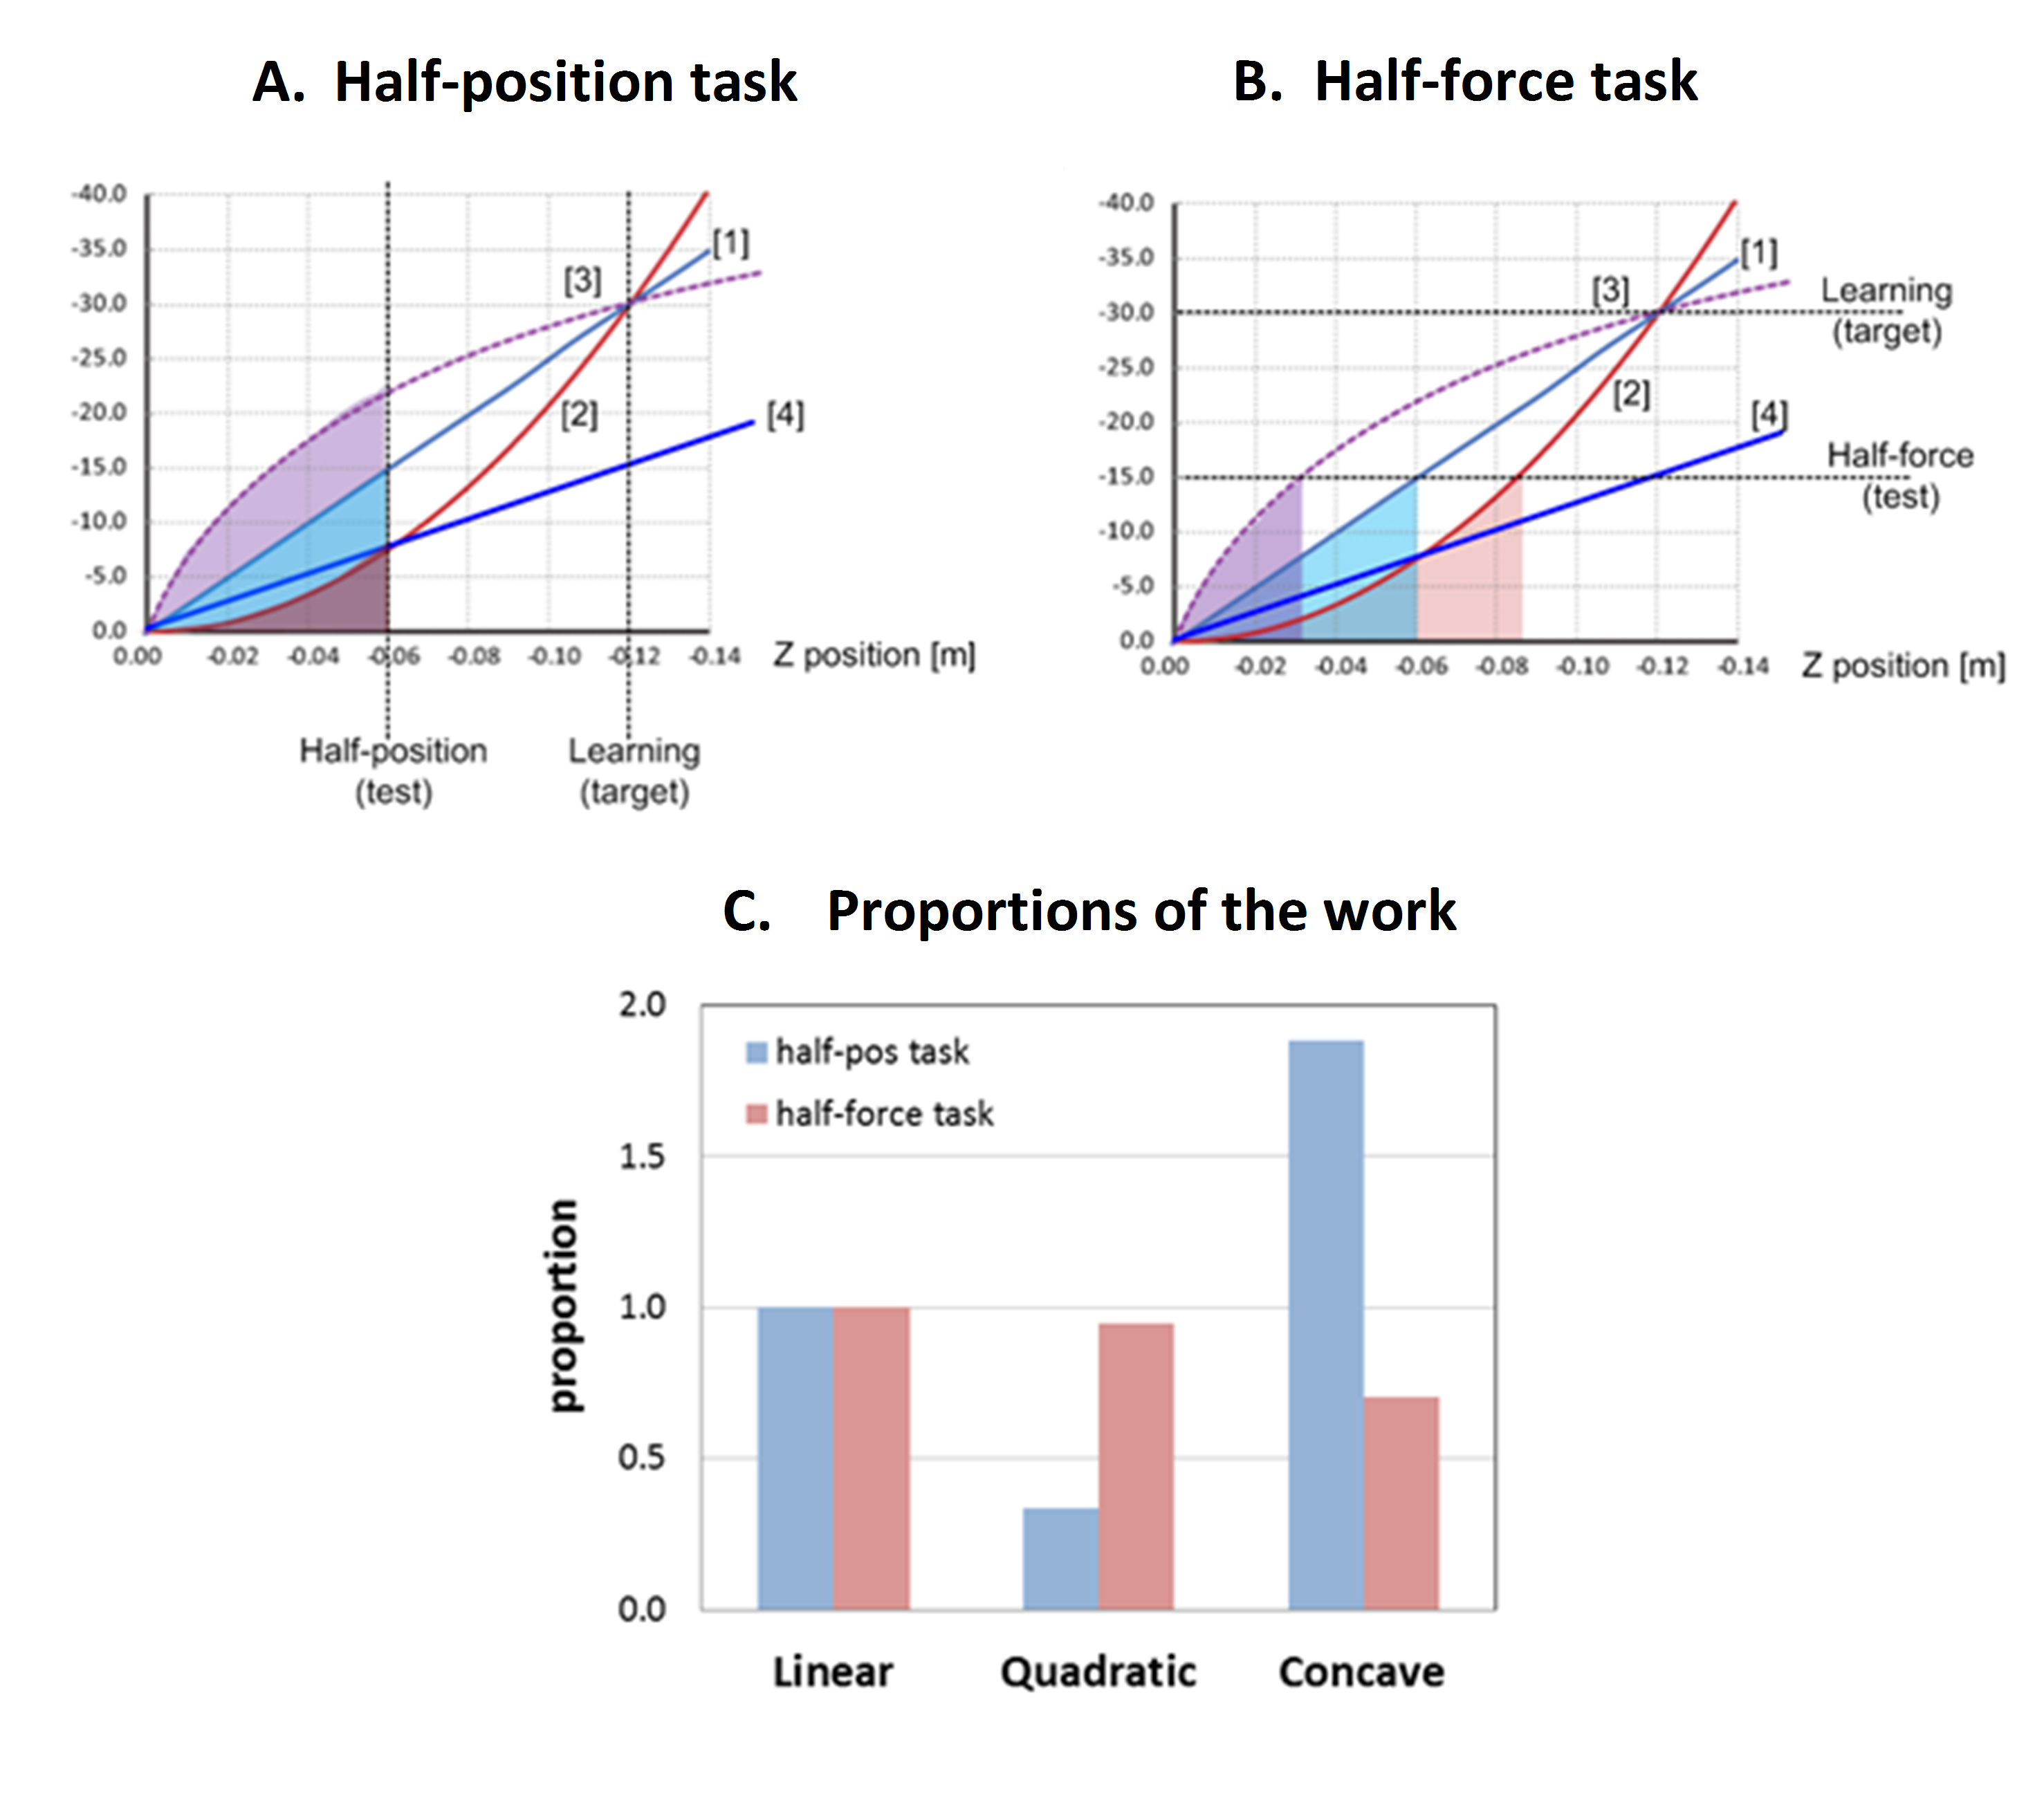
\includegraphics[width=.7\textwidth]{Chie/figs/Figure10.png}
	\caption{Illustrations to explain the Work differences for the half-position task (A) and the half-force task (B). Coloured areas represent the Work depending on the force dynamics. C. the bar charts of the proportion of the work when linear work is 1.0. }
	\label{work}
\end{figure}
The definition of “Work” is the result of object movements against force. Work of a force can be calculated by the line integral of its scalar tangential component along the path (from z1 to z2).

%
\begin{equation}
\BW = \int_{z1}^{z2} f(z) dz
\end{equation}
%

Based on the Figure 4, the Work should be different between three different forces.
Figure 10 shows that there are significant differences on the Work when conducting half-position task than half-force task.

Based on the measurements (position, velocity, and force for each conditions), we calculated the temporal aspects of the tasks with the different force dynamics.
%
\begin{equation}
\BW = \int_{t1}^{t2} fz Vz dt
\end{equation}
%

In Figure 11, the similar pattern between three force dynamics can be seen for the all the three sessions: learning, half-position, and half-force tasks. Such energy pattern might affect the half-force task performance and some participants might set the end-effector at half-energy they felt rather than the half-force itself. This pattern can be confirmed by the significant differences between the three forces in Figure 8. Humans might be not good at the point perception of the force, but the brain might be better understanding of the total cost and employ it to estimate/predict the “half” force ruled by the energy. To evaluate these possibilities, we need further data analyse and may be required to conduct additional/supplemental experiments.
%
\begin{figure}
	\centering
	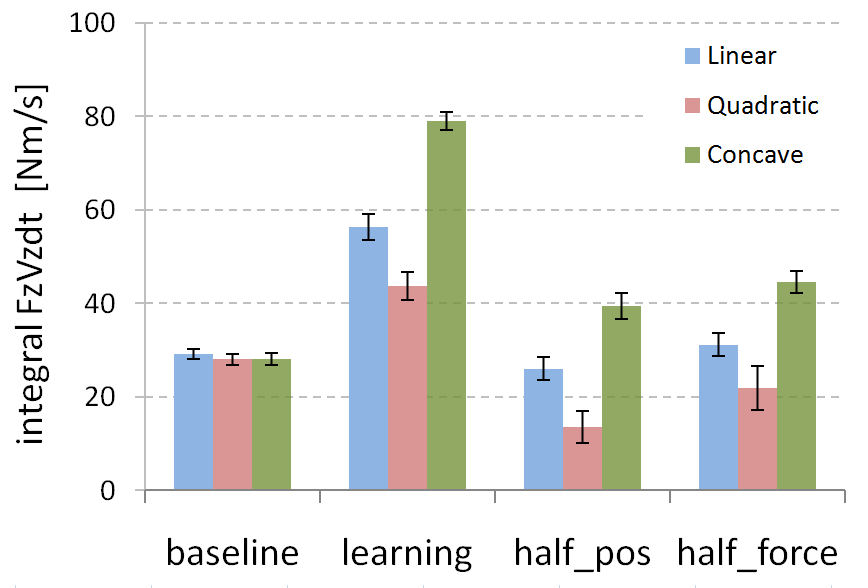
\includegraphics[width=0.7\textwidth]{Chie/figs/Figure11.png}
	\caption{The calculations from the measurement values (force and velocity) from start to the end points at the test trials, averaged across 18 participants.  Note: in the baseline block, only the half-liner force was applied.}
	\label{forcevel}
\end{figure}

\subsection{Dynamic learning evaluation}
The dynamic learning performance of human reachability tasks was evaluated and the results of 18 participants are presented and discussed in this section. The sequences of the three forces which are applied are different for each user (the order was pseudo-randomly assigned to the subjects and well counter balanced between them.) This consideration could help in understanding the role of each force models and the learnability for three different forces and also to see whether they affect any part of the learning model.

In the learning session, the user repeated the target reaching movement for n=50 trials. The averaged learning performance of the 18 participants depicted the behaviour pattern observed against a target position reached and maintaining them at a constant 0 velocity at the end the movement. 
In the analyses, we set the parameters to the equation (2) as below.
$Z_d=0.12  m;\dot{Z_d}=0.0  m/s;K=0.05 s ;$
K is a constant value defined as function of the output sampling rate.

The K value is defined as function of the output sampling rate (in Simulink). The goal of this analysis is to observe the number of trials needed for each user to reach the target position and also maintaining a zero velocity at the end position, resulting in M=0. The analyses resulted in the averaged values of the deviation in the learning metric values with respect to the different forces $(mean\pm \sigma)$.

$Linear: 0.00288 +/- 0.00358;$ 
$Quadratic: 0.00226 +/- 0.00213;$
$Concave: 0.003289 +/-  0.003559;$ 

From the learning evaluation, it is also evident that the participants were gradually improving the precision within a minor range of deviation. The standard deviation results are also monitored with respect to all the users and represent the participants’ performance with respect to the different contact forces presented to the user. 

The learning curve also expresses the concave as an unusual or unnatural force and the learning performance is quite different in comparison with the linear or quadratic force. The quadratic force performance resulted in a better behaviour in reaching the target position more precise and to maintain them at zero. Linear model performance converged to a lesser value within a span of 5 trials while concave resulted at the end of 10 trials. 

The learning performance analysis of all the users showed that Concave force is not natural or in other words it needs several repetitions to understand the dynamics and to learn how to maintain the accuracy in reaching a target, Figure 12. For Linear force, the performance is better but still the learning never converges to zero, indicating the progress and deviation in the learning model. For quadratic, the learning curve is more near to zero which indicates the improvement in being more accurate. Indicating that the users learnt the quadratic force better than linear forces, in other words quadratic force is easy and more natural force to learn, verified by the position accuracy at the target position. 
%
\begin{figure}
	\centering
	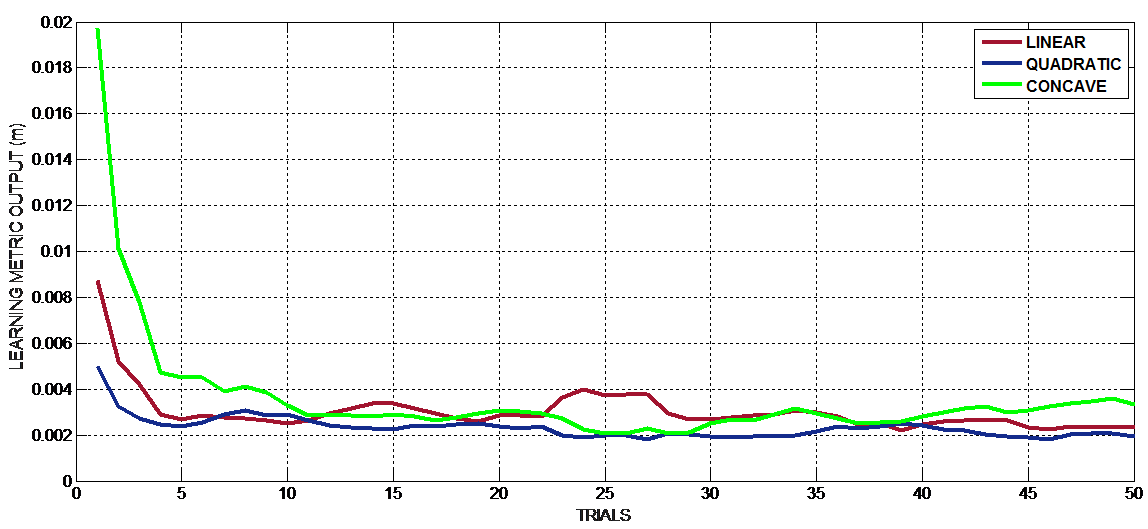
\includegraphics[width=.7\textwidth]{Chie/figs/Figure12.png}
	\caption{Averaged learning performance of the 18 participants over 50 trials in the learning phase of three different forces.}
	\label{learning}
\end{figure}
Figure 13 illustrates the standard error observed in each trial. The deviation of the learning metric value does not vary much especially in case of quadratic force. However, in both linear and concave forces the deviation seems to be varying depend on the number of trials or repetitions. This could be a result of the speed in reaching the target position or fatigue.
%
\begin{figure}
	\centering
	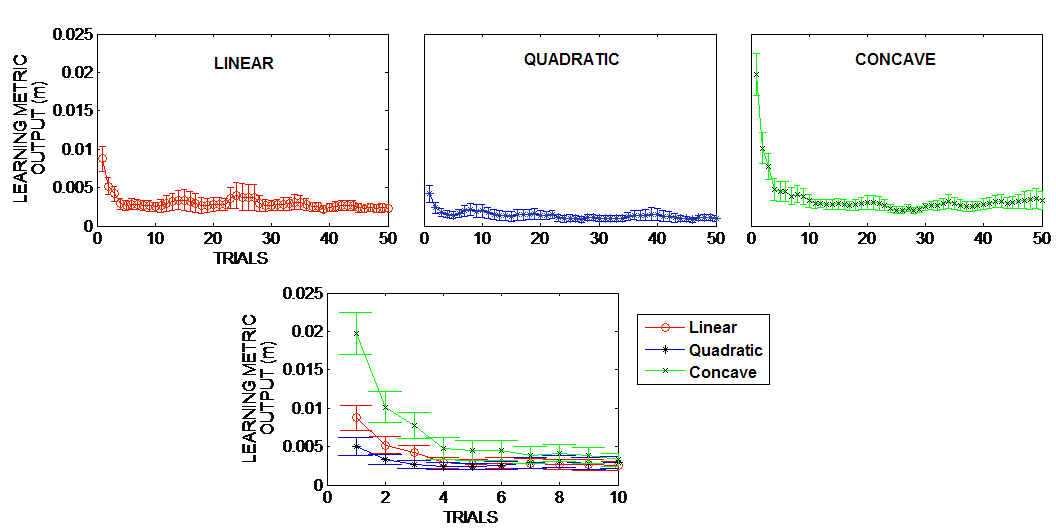
\includegraphics[width=0.7\textwidth]{Chie/figs/Figure13.png}
	\caption{ Learning performance of the 18 participants along with the standard error. A big variation in the learning performance of the three different forces is observed within the initial 10trials.}
	\label{learnerror}
\end{figure}
Metric evaluation results of the learning performance of  participants,
\begin{enumerate} 
	
	\item Concave force seems to be more un-natural, based on the learning curve variance.
	
	\item Linear force has less errors but the learning model maintains a stable condition after n trials, assuming that the learning is good but with the constant overshoots in position. 
	
	\item	Quadratic force seems to be a “well known” force but still the performance gradually improves over the course of trials. The force model helps the user to achieve more precise and accurate movements. 
	\end {enumerate}
	
	The time taken to reach the target position or the distance covered is also plotted to understand the specific behaviour of the different learning performance, as shown in Figure 14. All the participants, irrespective of their gender or dominant hand, approached the quadratic force with longer time and being more considerate in reaching the target position. In case of linear and concave model the participants tend to approach the target more rapidly which again resulted in the lack of judgement in being more precise and not learning to reach the target position accurately. Since both the linear and concave model had an increased contact force at the initial stages it can be a result of the same in reaching the target.
	%
	\begin{figure}
		\centering
		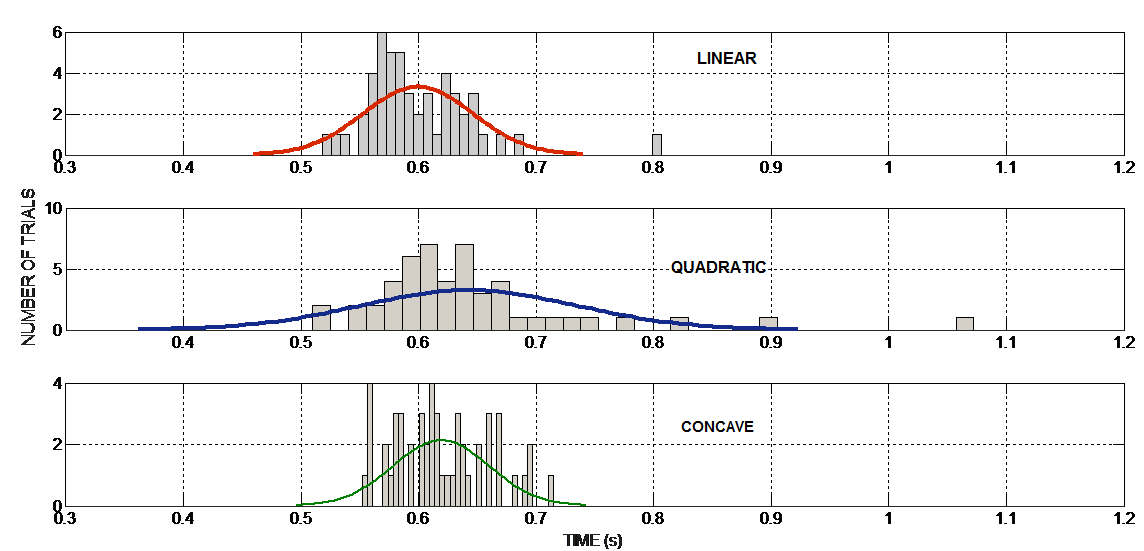
\includegraphics[width=0.7\textwidth]{Chie/figs/Figure14.png}
		\caption{Average Time taken by the 18 participants to reach the target Z=0.12m with the three different forces }
		\label{speed}
	\end{figure}
	The Probability distribution of the time for different force models are presented here, 
	\begin{enumerate}
		
		\item	Quadratic force model is very fragile but still the time reaching the target is quite wide range
		
		\item	Both Concave and Linear have a similar behaviour in terms reachable time. 
		
		\item	Although the initial force is high in concave model the time taken to reach the target is quite low- which will explain the higher over shoots. 
	\end{enumerate}
	
	This time also explains the learning capability of the force dynamics, lower force takes longer time than the higher force.
	
	\subsection{Questionnaires}
	The responses for both the questions can be shown in Table 3 and Figure 15. The Table provide individual responses with their demographic information and the two bar charts illustrate the averaged data across 18 participants.
	
	The Table 3 showed that majority of the participants $(55.5\%)$ could not differentiate between linear and non-linear forces.  $44.5 \% $of the participants succeeded in identifying the difference between a linear and non-linear accurately.
	\begin{figure}
	\centering
	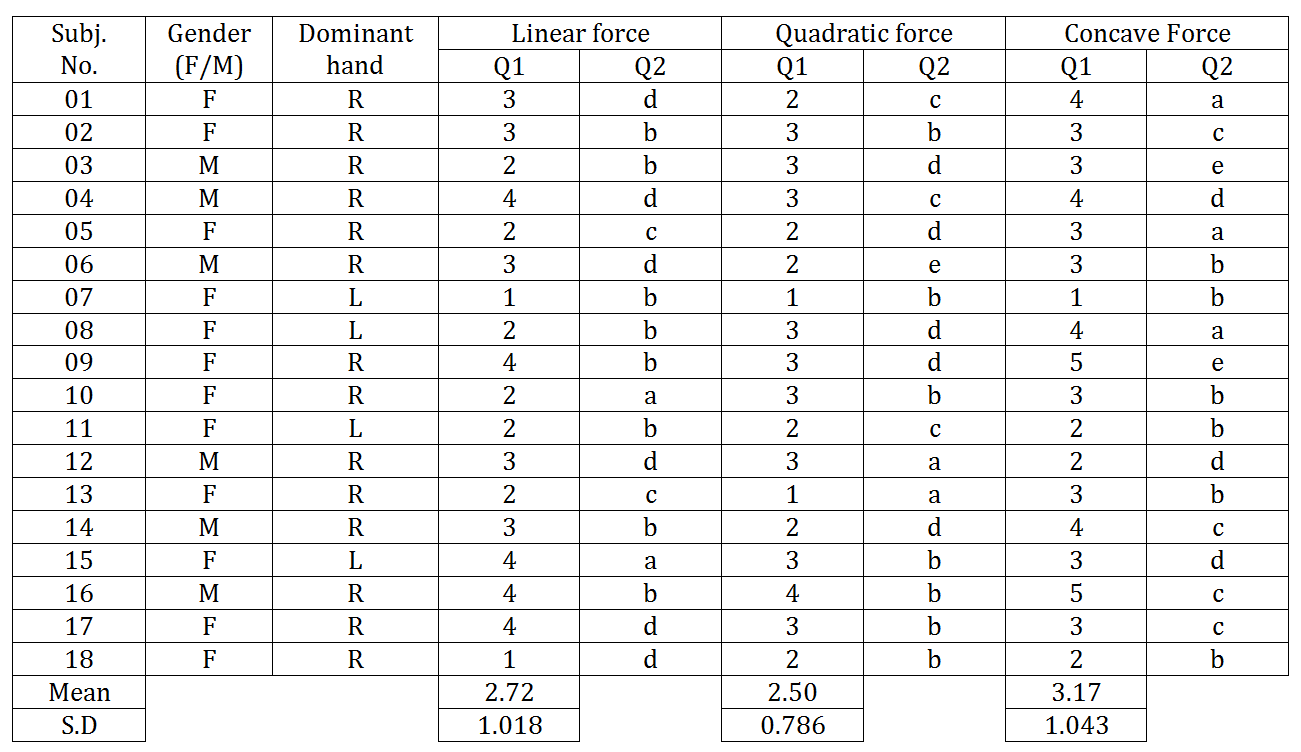
\includegraphics[width=0.7\textwidth]{Chie/figs/Table3.png}
	\caption{Participant demographic information and the questionnaire responses}
	\label{Table1}
\end{figure}

According to the Figure 15, participants rated more effort on to the Concave force after the session.
A statistical analysis was made for the results of the Q1. Mauchly’s test of Sphericity indicated that the assumption of sphericity had not been violated, $\chi^2 (2) = 0.287, p = .866$. A repeated measures ANOVA showed that mean effort differed significantly between three type of forces, $F(2,34) = 5.633, p = .008 < .05$. Post hoc tests using the Bonferroni correction revealed that the mean difference was only significantly between the Quadratic and the Concave (p = .019).
%
\begin{figure}
	\centering
	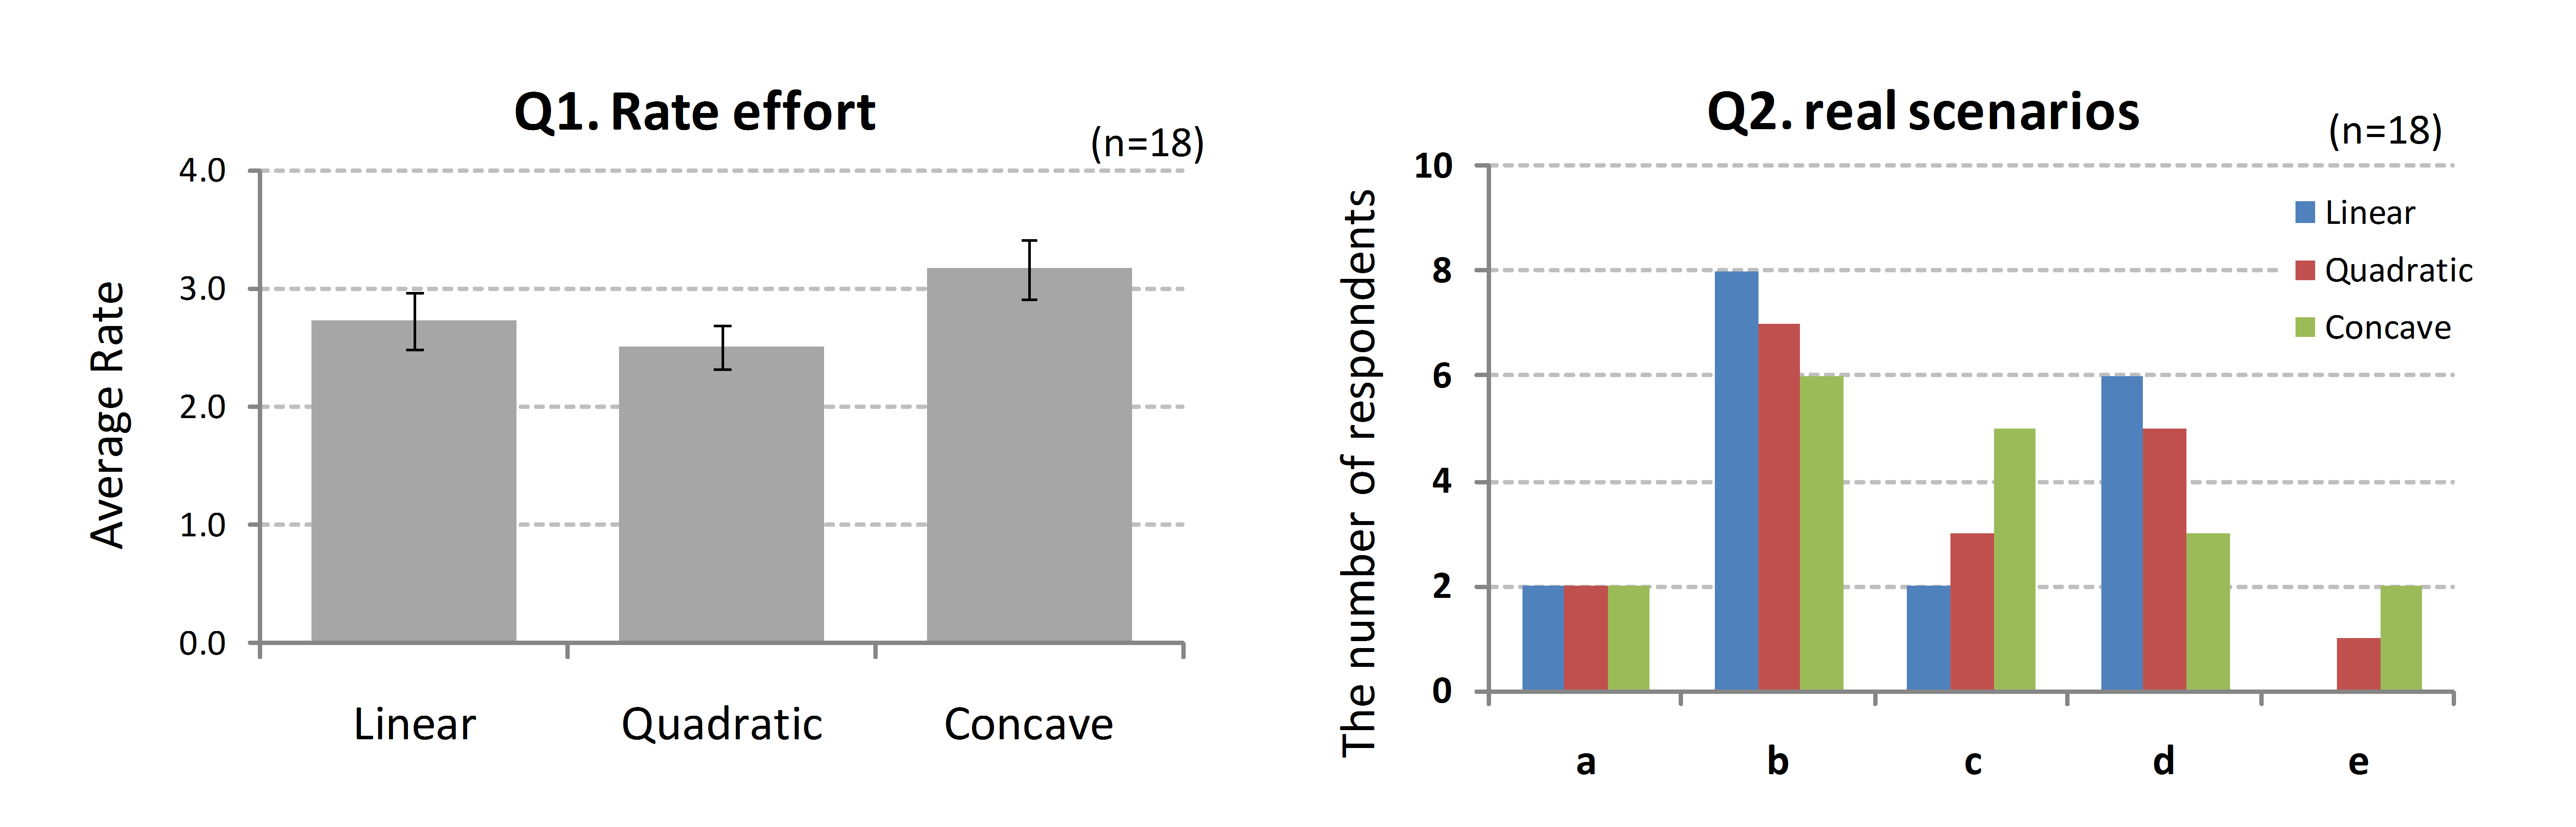
\includegraphics[width=0.7\textwidth]{Chie/figs/Figure15.png}
	\caption{Q1. Average rate of the effort for three different forces across 18 participants. Q2. The number of respondents considering five real scenarios: a. cushion, b. revolving door, c. box on a plane surface, d. hinged door, e. a box on an inclined surface.  See more details at the Method section. }
	\label{questionnaire}
\end{figure}
It is hard to analyse the results of the Q2: real scenarios, and to examine the correlation between the Q1 and Q2. The number of participants was only 18, and their individual differences on the force perception seemed to be larger than their differentiation among three types of forces. Also, their force perception might have strongly affected by the task itself rather than the force type itself. Even though there were difficulties to interpret the responses, the Q2 bar graph indicated that some pattern clearly existed among three forces. There are possible ways to make further analyses; for example, to increase the number of participants and to evaluate the perception differences from their normalised (baseline) performance. This is a challenging research theme but very important in this research area. Further analysis should be made to bridge between physical properties and subjective human force perception.
\clearpage{}

\chapter{Towards engagement models that consider individual factors in HRI: on the relation of extroversion and negative attitude towards robot to gaze and speech during a human-robot assembly task}\label{sec:Serena}
\setcounter{figure}{0}
%\thanks
%{This work was performed within the project EDHHI of Labex SMART (ANR-11-LABX-65) supported by French state funds managed by the ANR within the Investissements d'Avenir programme under reference  ANR-11-IDEX-0004-02. The work was partially supported by the FP7 EU projects CoDyCo (No. 600716 ICT 2011.2.1 Cognitive Systems and Robotics).}}

%\author{Serena Ivaldi \and Sebastien Lefort \and Jan Peters \and Mohamed Chetouani \and Joelle Provasi \and Elisabetta Zibetti}


%\institute{S. Ivaldi \at
 %             Inria, Villers-l\`es-Nancy, F-54600, France\\
%	Loria, CNRS \& Universit\'e de Lorraine, Loria, UMR n. 7503, Vandoeuvre-l\`es-Nancy, F-54500, France\\
%		Intelligent Autonomous Systems, TU Darmstadt, Germany\\
%             Tel.: +33-03-5495-8508\\
%            \email{serena.ivaldi@inria.fr}           
%        \and        
%       S. Lefort \at          
%      LIP6, Paris, France          
%     \and          
%    J. Peters \at
%   Intelligent Autonomous Systems, TU Darmstadt, Germany\\
%  Max Planck Institute for Intelligent Systems, Germany         
%           \and                   
%	M. Chetouani \at
%	CNRS \& Sorbonne Universit\'es, UPMC Universit\'e Paris 06, Institut des Syst\`emes Intelligents et de Robotique (ISIR) UMR7222, Paris, France%\\
%	%CNRS, Institut des Syst\`emes Intelligents et de Robotique UMR7222, Paris, France
%	\and
%	J. Provasi \and E. Zibetti \at
%	CHARt-Lutin, Universit\'e Paris 8, Paris, France}



\section{Introduction}
Service and personal robots must be capable of cooperating and interacting with humans for a variety of tasks.
The robot's social skills are crucial to prevent the interaction to become cumbersome and the cooperation less effective.  
Social signals, i.e., verbal and non-verbal cues produced by the human and directed towards the robot, may reveal the engagement and ease of the person during the task, whether or not a physical interaction is entailed \cite{Anzalone2015engagement,ivaldi2014frontiers,Chen2014NARStouch}.

The ability to estimate engagement and regulate social signals is particularly important when the robot interacts with people that have not been exposed to robotics, or do not have experience in using/operating them: a negative attitude towards robots, a difficulty in communicating or establishing mutual understanding may cause unease, disengagement and eventually hinder the interaction.

\begin{figure*}[ht!]
	\centering
	{
		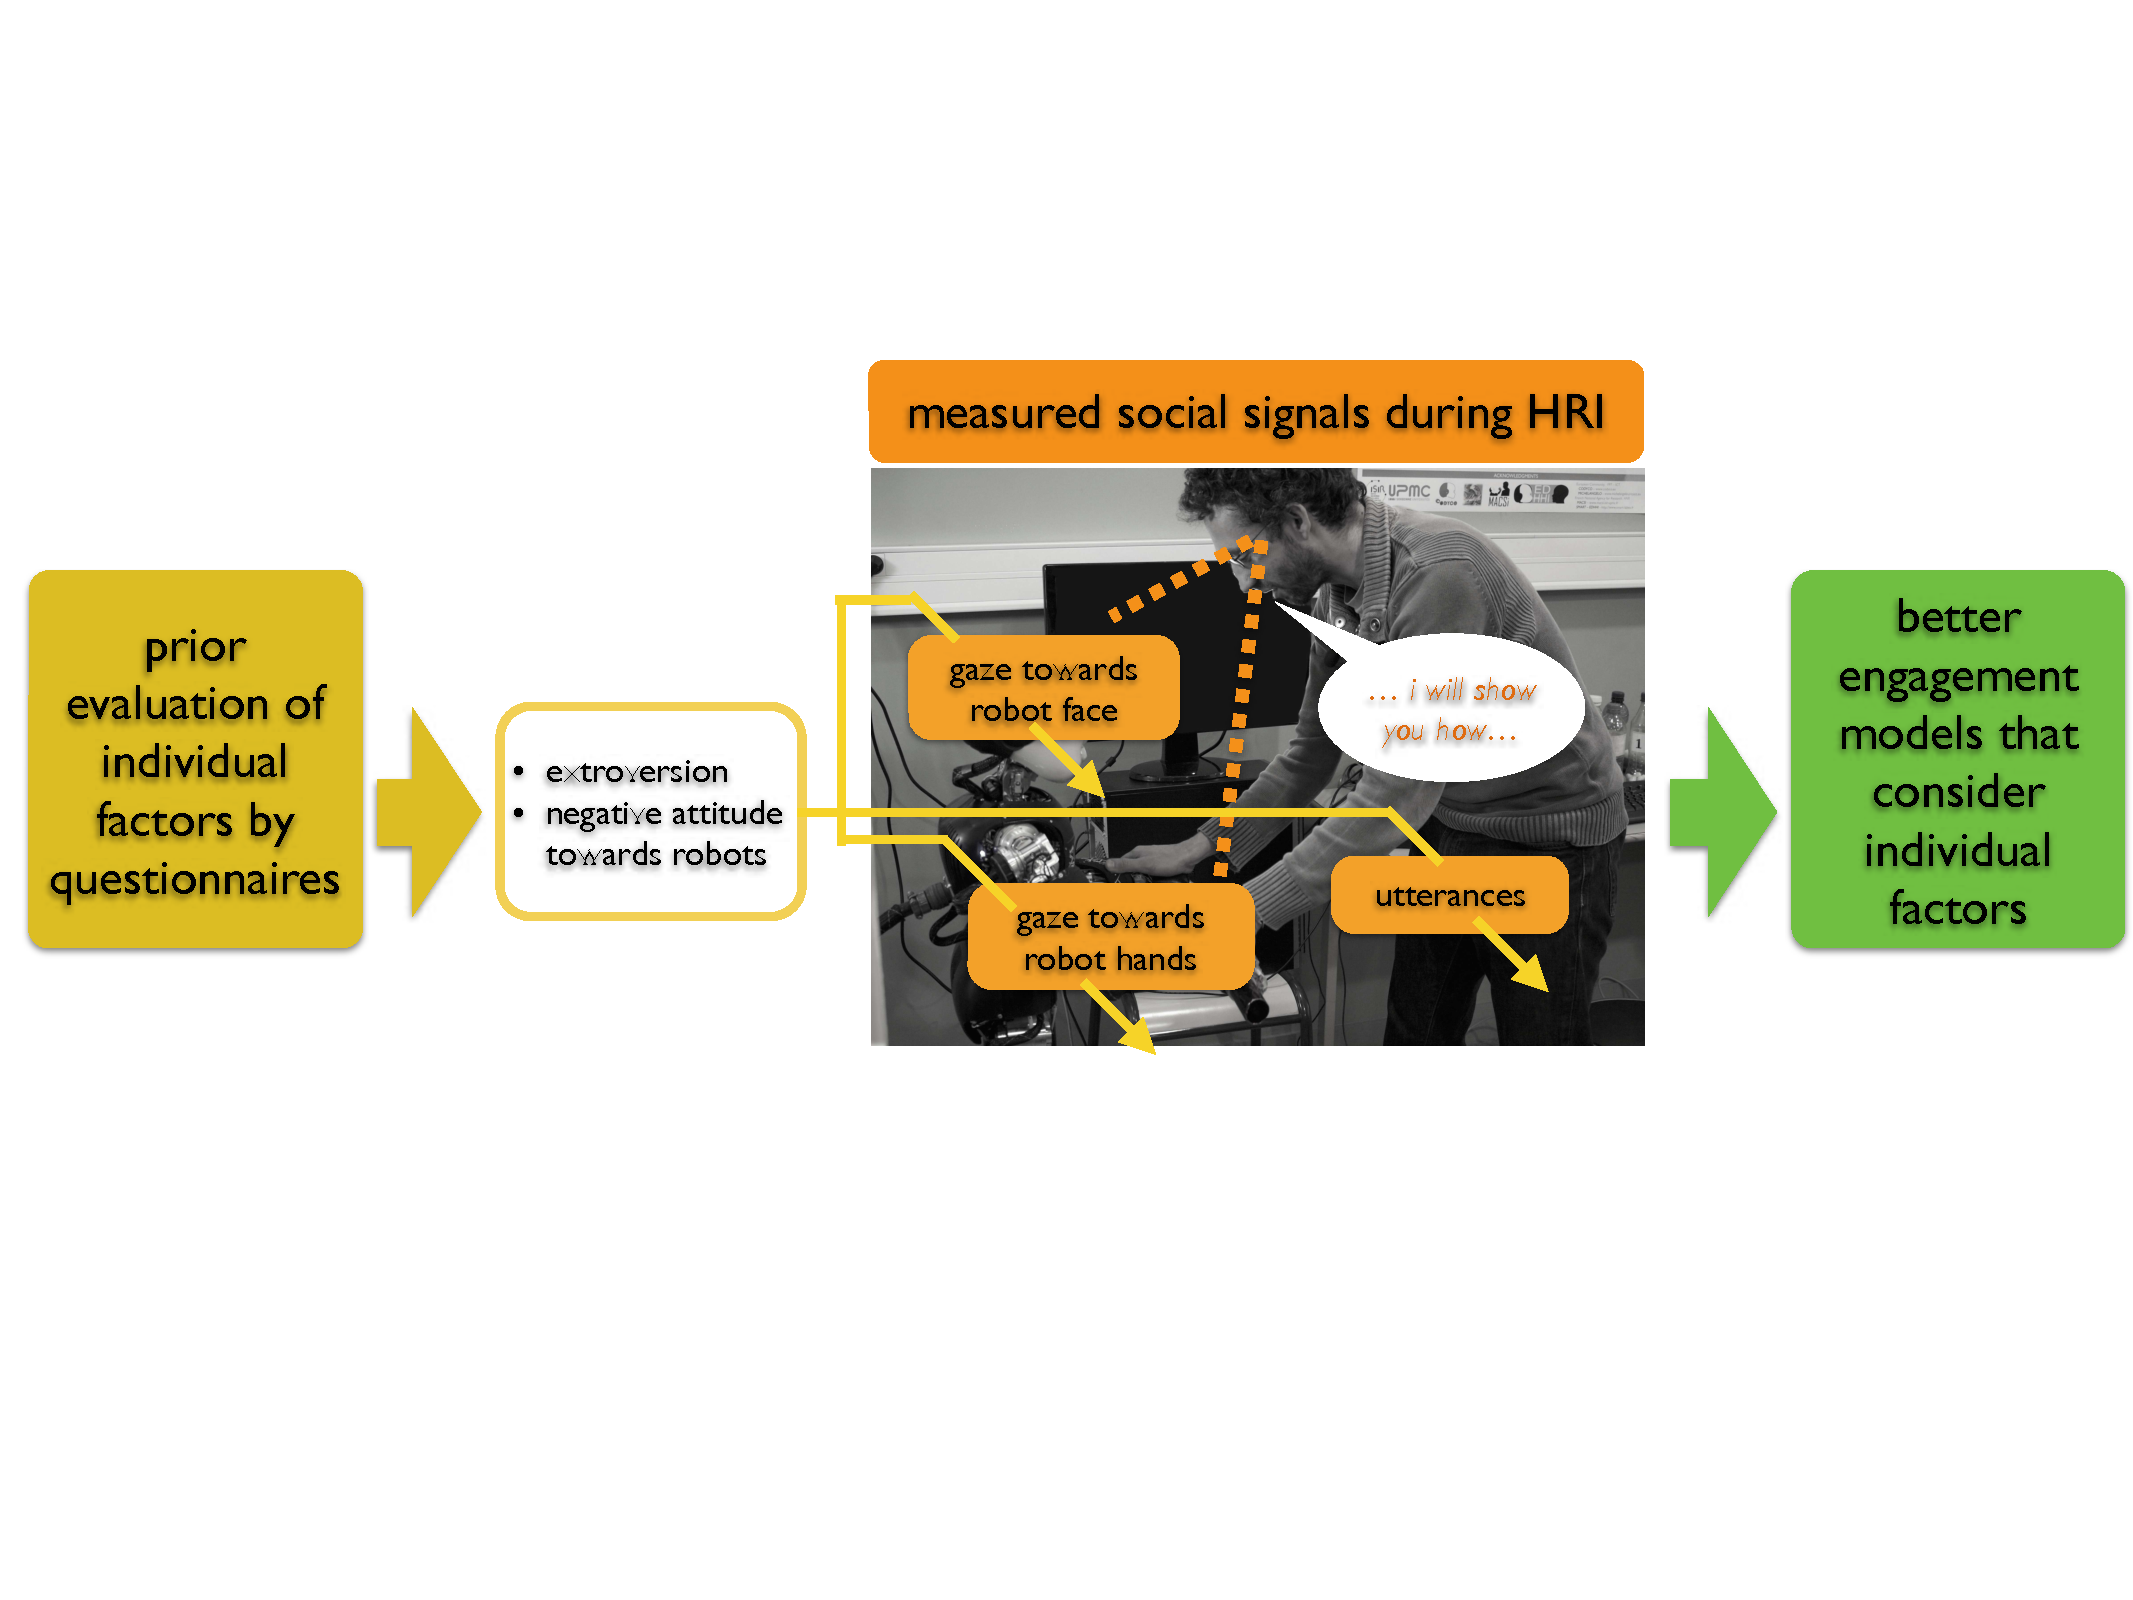
\includegraphics[width=0.8\hsize]{Serena/figures/conceptual6.pdf}
	}
	\caption{Conceptual representation of the experiment: we study the relation of extroversion and negative attitude toward robots on speech and gaze during a cooperative assembly task.}
	\label{fig:concept}
\end{figure*}

It seems therefore necessary to study how individual and social factors influence the issue of social signals during human-robot interaction, together with their relations to acceptance and engagement.


To evaluate the engagement during human-robot interaction, the most common metrics are based on the temporal dynamics of social signals, in particular gaze and speech \cite{Anzalone2015engagement,rich2010recognizing}.
The exchange of gaze (mutual and shared), the contingency of reactions to speech and gaze cues, the temporal dynamics of speech (utterance number, frequency, duration) are among the most common indicators of engagement during dyadic tasks \cite{ivaldi2014frontiers}.


However, there is evidence from the psychology literature that the dynamics of these social signals can be altered by individual factors \cite{LaFrance2004,Iizuka1992,Scherer1981}: we refer here to the set of behavioral, emotional, and cognitive tendencies that people display over time and across situations and that distinguish individuals from one another, such as personality traits and social attitudes.
The influence of personality traits on human behaviors during interactions with robots has been also documented in several studies \cite{Takayama2009proxemics,Dang2014personality,Aly2013personality}. 

Two individual factors seem particularly interesting for HRI: extroversion, a personality traits that is associated to positive emotions and social behavior \cite{BIGFIVE}, and negative attitude towards robots \cite{NARS2006}, a personal attitude that captures the projected anxiety of the person toward the interaction with a robotic device. 
Recent studies showed that there is a correlation between these traits/attitudes and the issue and dynamics of social signals, in particular gaze and speech \cite{Nomura2008}.
In this case, if they impact the issue of such social signals, they also affect the power of the metrics used as indicators of engagement.

%Following this rationale, 
Following this line of thought, the goal of this work is to study the relation between individual factors (extroversion and attitude toward robots) and the dynamics of gaze and speech produced by the human during an interaction with a robot (see Figure \ref{fig:concept}).

For this purpose, we designed a collaborative assembly task between a human and a robot. We made video and audio recordings (see Figure \ref{fig:setup}) of the interactions between the humanoid robot iCub and adult participants who previously submitted their questionnaires for evaluating the extroversion and negative attitude towards robots\footnote{In social psychology, there is a net distinction between personality traits and attitudes. Here, we use methods from differential psychology rather than social psychology: the distinction between the two is not important, as long as the two factors are two characteristics of the individual that are evaluated at a certain time prior to the interaction. We measured the attitude towards robots with the NARS questionnaire, a test that was created to capture the projected anxiety of the person before its interaction with the robot. We used it to evaluate an individual attitude prior to the direct interaction with the robot (participants filled the NARS questionnaire several days before the experiment - see details about the experimental procedure in Section \ref{section:protocol}).}. 
The questionnaire scores were later used to study the issue (frequency and duration) of utterances and gaze towards the robot issued by the human partner. Since our experiment also involved a physical contact between the robot and the person during the assembly, we distinguished between gaze towards the robot face and gaze directed towards the robot's hands, that perform the assembly thanks to the human guidance.


Our study shows that, at least for the cooperative assembly task, there is a correlation between extroversion score and the speech frequency and duration, while the negative attitude is related to the duration of gaze towards the robot. To summarize:
\begin{itemize}
\item \emph{the more one is extrovert, the more he/she will talk to the robot}
\item \emph{the more one has a negative attitude towards a robot, the less he/she will look at the robot face and the more he/she will look at the robot hands, where the physical interaction for the assembly takes place}
\end{itemize}

As gaze and speech are the main social signals used to evaluate engagement \cite{rich2010recognizing}, we provide significant results supporting the idea that engagement models used in HRI should take into account individual factors that can influence the production of such social signals.

By gaining a deeper understanding of the inter--individual factors that influence the exchange of gaze and speech during cooperative tasks, we aim at improving the design of robot controllers during social and physical interaction.
More generally, we would like to turn our findings into implications for the design of robot controllers that can adapt to the individual differences of the human partners.




%=================================
%=================================
\section{Background}\label{sec:background}



\subsection{Social signals: the building blocks for assessing engagement}




\begin{table*}
\resizebox{\textwidth}{!}{%
\centering
\begin{tabular}{|p{4.5cm}p{0.7cm}p{11cm}|}
\hline
Study & Ref & Social signals used to assess the engagement \\
\hline
\hline
Castellano et al., 2009 & \cite{Castellano2009} & Gazes towards the robot\\
 				& & Smiles\\
\hline
Ishii et al., 2011 & \cite{Iishi2011} &Gazes Towards the object the agent is talking about \\
			& &Gazes Towards the agent's head \\
			& &Gazes Towards anything else \\
\hline
Ivaldi et al., 2014 & \cite{ivaldi2014frontiers}  &Reaction time to the robot attention utterance stimulus \\
												& &Time between two consecutive interactions\\
\hline
Le Maitre and Chetouani, 2013 & \cite{Lemaitre2013} &Utterance directed to the robot \\
						& &Utterance  directed to self \\
\hline
Rich et al., 2010	& \cite{rich2010recognizing} &Gazes Focused (man and robot are looking at the same object \\
					& &Gazes Mutual (man and robot look at each other) \\
					& &Utterance Adjacent (two successive locutions, produced one by the robot, the other by the human, separated by a maximum interval) \\
					& &Utterance Responses (the subject responds to the robot through a gesture or a very short verbal intervention) \\
\hline
Sanghvi et al., 2011 & \cite{Sanghvi2011} & Postures (curve and inclination of the back) \\
\hline
Sidner et al., 2004 & \cite{sidner2004} &Gazes Shared (mutual or directed) \\
 			  & &Gazes Directed towards the robot without the latter looking at the human \\
\hline
Sidner et al., 2005 &  \cite{sidner2005} &Gazes Shared (mutual or directed) \\
 			  & &Gazes Directed towards the robot without the latter looking at the human \\
\hline
\end{tabular}}
\caption{Social signals used in literature as metrics for the assessment of engagement.}
\label{table:literature}
\end{table*}


During interaction, a multitude of verbal and non-verbal signals are exchanged between the two partners. These so called \textit{social signals}  and their dynamics are the main bricks for the evaluation of the \textit{engagement} in HRI.

The engagement is defined as ``the process by which individuals involved in an interaction start, maintain and end their perceived connection to one another'' \cite{sidner2005}. As discussed in \cite{Anzalone2015engagement}, the engagement is related to the user experience, to the perceived control, feedback, interactivity, attention, and the fluctuations of the engagement during interaction are reflected into physiological changes and behavioral changes through verbal and non-verbal communication.

A social signal may be defined as ``a communicative or informative signal, or a clue which, directly or indirectly, provides an information about social facts, i.e. interactions, emotions, attitudes, valuations or social behaviors, social relations or identities'' \cite{Poggi2012}. The scope of social signals potentially extends to a large variety of behaviors and expressions: gestures, facial expressions, postures, gazes, etc. 
Anzalone et al. \cite{Anzalone2015engagement} partition the set of metrics for engagement evaluation into static and dynamic features. The first set comprises focus of attention and gaze analysis, head and body postural stability, with evaluation of pose and variance. The second set comprises joint attention, reaction times to attention cues, imitation, synchrony and rhythm of interaction. 

To assess the engagement during HRI experiments and tasks, researchers usually considers a subset of these social signals (see Table~\ref{table:literature}), frequently focusing on gaze and speech.


Gaze is one of the most important cues and carriers of information during the interaction.
It is indeed well established that mutual gaze and eye contact are crucial during human-human interaction \cite{Goffman1967}: the absence of eye contact at the right time, for instance at the end of a sentence, can be perceived as a withdrawal from the conversation and a sign of disengagement. 
Gaze in HRI can be analyzed differently depending on its direction and target.
For example, during verbal interaction \cite{rich2010recognizing,Iishi2011} or learning games \cite{ivaldi2014frontiers} it can be mutual (when the robot and the human partner look at each other) or directed/joint (when the robot and the human look at the same object or in the same direction).  
A third type of gaze can be the one directed by the human towards the robot, that the latter can return or not, depending on its joint attention skills \cite{sidner2004}.
 
Speech, and more specifically the dynamics of verbal exchange (e.g., turn-taking), is the other most important social signal for interaction, and it is a crucial indicator in the assessment of engagement \cite{Lemaitre2013,rich2010recognizing}. The metrics used for evaluating the engagement using this signal are for example the number, frequency and duration of utterances \cite{Iishi2011,rich2010recognizing}, the reaction time to utterance cues \cite{ivaldi2014frontiers}. Le Maitre and Chetouani \cite{Lemaitre2013} also proposed a qualitative distinction between language actions involving the locutions directed towards the robot, and those towards oneself.


Body language, which includes non-verbal behaviors such as facial expressions, posture and gestures, can also convey the intention and the engagement of the human partner. 
For example, Sanghvi et al. \cite{Sanghvi2011} analyzed the individual postures (the inclination and curve of the back) and their changes to assess the engagement of children playing chess against a humanoid robot.
%Therefore, in HRI, engagement can be revealed 
The engagement was also studied in relation to positive facial expressions (e.g., smiles rather than grins) \cite{Castellano2009}, head movements such (e.g., nodding) \cite{Sidner2006} and gestures responding responding to a robot cue \cite{rich2010recognizing}.


To summarize, there are numerous studies that characterize the engagement and the interaction between humans and robots through the analysis of verbal and non-verbal signals. However \emph{gaze and speech are the most common social signals used to evaluate the engagement}, as clearly showed in Table \ref{table:literature}.

Since the engagement is a sort of emotional ``state'' of the human partner during the social interaction, and it may fluctuate over the interaction, it is interesting to study the  temporal dynamics of the social signals and the salient events associated to their evolution during the interaction. 
To estimate the engagement in HRI using the exchanged social signals, there are two main approaches in the literature.

The first approach consists in assessing the engagement of the human partner in real time. For instance, with a probabilistic approach Ishii et al. \cite{Iishi2011} demonstrate that a certain sequence of three gazing primitives (towards the object designated by the agent, towards the agent and towards any other direction) can reliably predict the human subject's withdrawal from an interaction. 
In their experiment, the robot was introducing a new model of mobile phone, and a sequence of gaze towards the robot then twice towards unrelated objects was linked to a disengagement.
 

In the second approach, that we may consider as ``global'', the engagement is neither measured in real time, nor on time intervals, but on the interaction as a whole. 
For instance, Sidner et al. \cite{sidner2004,sidner2005} suggest a metric combining the shared gazing time and the time spent by the subject looking at the robot for the whole duration of the interaction on one hand, and the assessment of the number of gazes that the participant returns to the robot during the same period of time on the other hand. 
With a similar approach, Rich et al. \cite{rich2010recognizing} developed a composite index defined by the average time intervals between two social connection events between the robot and the user in the course of an interaction, where the robot had to teach the participant how to prepare cookies. According to the authors, the events were divided into four sorts: 1) directed gaze, 2) mutual gaze, 3) adjacent utterances when two are produced in succession, one by the robot and one by the participant, with a maximum time gap between them, and 4) the replies to the robot with a gesture or a very short utterance. 
%In these works, the research groups of Sidner, Rich and colleagues \sl{Attention, ce ne sont pas les memes papiers} 
In the aforementioned studies, the researchers also observed the effect of various cues of the robot (e.g., robot nodding vs. not nodding) on the engagement of the user during the interaction.
A specific approach on the whole interaction was proposed by Le Maitre and Chetouani \cite{Lemaitre2013}: they proposed the ratio between the talking time directed towards the robot and the one towards oneself as indicator of engagement, with the rationale that an increased verbalization directed towards the robot can be interpreted as a stronger engagement (whereas the more the people talked to themselves, the lesser the engagement). 

To summarize, both considering the whole interaction and thin slices of interaction, measuring the engagement in HRI relies on the dynamics of the exchanged social signals, particularly gaze and speech.

However, there are no models that take into account context, task, social or individual factors that may affect the production of such signals, and subsequently the evaluation of the engagement. 

To the best of our knowledge, the HRI literature considering the inter-individual differences (concerning the personality) or the attitude (positive or negative) towards robots in the production of those signals is scarce. 
When discussing models of engagement, the human individual is considered as ``abstract'', expected to produce the same social signals at the same rhythm, despite any inter-individual difference that may affect the communication, the establishment and the continuation of the social interactions. 

It is however rational to consider that there can be personality traits, dispositions or attitudes that can make people talk, look and behave in a different way when facing the same interaction, especially with a device such as a robot.
For example, an introvert individual may talk less to or look less at the robot than an extrovert individual, without however being necessarily less engaged than the other. 
An individual with negative attitude towards robot may look less at the robot face, and look more at the robot's body, especially during close or physical interactions with the robot.
In short, the effect of  personality characteristics and of the attitudes towards robots could impact the dynamics of social signals, and subsequently undermine the metrics and models used in the literature to assess the engagement in HRI.


\subsection{Personality traits and attitudes}


As explained by Ajzen \cite{Ajzen1986}, ``attitudes and personality traits are latent, hypothetical dispositions that must be inferred from observable responses''. Their effect should be therefore observable on the overt actions of the individual.
The boundary between traits and attitudes is under debate; however it is acknowledged that both attitudes and personality traits influence our actions and behaviors, together with other social, contextual and individual factors \cite{Scherer1981}.
To make it simple, a personality trait is a characteristic of the human personality that leads to consistent patterns of behaviors, and is assumed to be almost invariant for an adult.
An attitude is a behavior tendency, directed towards people, objects, situations, and is generally determined by the social context, the background and experiences of the individual \cite{Wood2000}.



\subsubsection{Personality trait: extroversion}

The personality of an individual consists of several characteristics and dispositions, each  being described as a ``gathering of attitudes obviously linked to each other, or as patterns of cognitive treatment of the information or underlying psycho-physiological mechanisms generating specific dispositions towards some behaviors'' (\cite{Scherer1981}, p.116).

Among the existing personality models, the most well-known and studied is the Big Five \cite{NEOPIR1998}, which owes its name to the five traits descriptive of a personality: \emph{Extroversion}, \emph{Neuroticism}, \emph{Agreeableness}, \emph{Conscientiousness}, \emph{Openness to Experience}. This model is widely used in psychology to predict human behavior and cognition \cite{Wu2014,Rauthmann2012}, and is more and more also used in human-robot interaction \cite{Tapus08,Takayama2009proxemics}.


%% extroversion
The extroversion dimension is the personality trait that notably (i) shows up more clearly during interaction, and (ii) has the greater impact on social behavior with respect to the other traits \cite{Zen2010}. It is linked to positive emotions, and identified through the tendency to be sociable, talkative, and self confident \cite{NEOPIR1998}. 
It seems to be fundamental to shape the way people interact \cite{Eysenck1981} and to establish and maintain social relations \cite{Wu2014}.
Beatty et al. \cite{Beatty2001} suggest that extroversion is one of the three major factors, together with neuroticism and psychoticism, that have some bearing on communication.  Moreover, it would also have an impact on the way individuals behave, and even on the quality of new social relations \cite{Berry2000}.

Although there is evidence in social psychology about potential links between the emission of various social signals (verbal and non-verbal) and the personality profile \cite{Argyle1976}, quantitative evidence is still needed. 
In particular, the current knowledge about extroversion and the issue of verbal and non-verbal signals is mostly limited to verbal dyadic and group interactions where there is typically no physical contact. 

Generalizing and characterizing the influence of individual differences and extroversion on verbal and non-verbal behaviors (e.g., gaze, head movements) is difficult \cite{LaFrance2004}; however, the literature in human-human interaction reports some evidence that the production of gaze and speech correlates to the level of extroversion of the individuals. 
For example, the level of extroversion has an effect on the frequency and duration of gazes towards a person during face-to-face conversations \cite{Iizuka1992}: extroverts gaze longer than introverts.
In a similar way, Wu et al. \cite{Wu2014} showed that extrovert individuals tend to focus their attention on the area of the eyes on pictures of human beings longer than introverts. 
The influence of personality traits, especially extroversion, on the gaze is also reported for non-social tasks such as fixating abstract images \cite{Rauthmann2012}. 

With regards to verbal communication, Costa et al. \cite{NEOPIR1998} noted that one of the most clear signs of extroversion for an individual is to be more talkative, which also leads to a lesser number of pauses during conversation \cite{Scherer1981}. Extrovert people would also tend to use shorter sentences at an increased rate than introvert people in informal situations involving another language \cite{Dewaele00}. 
The link between extroversion and speech dynamics was exploited for automatic classification of personality from videos of interaction between small groups of people: in \cite{Pianesi08,Lepri2010} the authors showed that the talking and interaction timing ratio are positively correlated to the level of extroversion.

To summarize, there is evidence from the literature on the influence of the extroversion trait on the dynamics of gaze and speech in human-human interaction. This certainly biases the current metrics and models for assessing engagement, that do not take into account such individual factors \cite{Anzalone2015engagement,rich2010recognizing}. 

Extending such studies to human-robot interaction, with the variability of tasks, situations and robots, it is certainly challenging. In this paper, we provide evidence that the dynamics of gaze and speech is related to the extroversion during a human-robot assembly task.





\subsubsection{Negative attitude towards robots}


As the literature seems to allege, extroversion may bring up inter-individual communication differences during social interactions between humans. While aversion towards other people may be identified through the personality models, there is currently no model that allows us to assess the dislike of technology, and more specifically robots. An individual may appear to be very sociable, while very wary of technology. 
For robots, this evaluation seems particularly critical. Currently, robots are diffused in factories and service and are mostly used or operate by skilled people that received some robotics training (i.e., experts). However, robots are gradually becoming available and accessible outside the classical settings, to ordinary people that have not received any robotics training (i.e., non-experts). Ordinary people without a proper knowledge of the platform are not typically aware of the limits and the real capabilities of the robots, because of their lack of prior experience with them and frequently limited background knowledge. 
Some people might be technophobic, some might have developed an anxiety towards robots, influenced by some recent trends in the public media\footnote{See for example the press article: ``Will workplace robots cost more jobs than they create?'' \url{http://www.bbc.com/news/technology-27995372}}, some may be influenced positively or negatively by movies\footnote{We interviewed our participants after the experiments. Some reported that they ``do not like robots because they are going to take our jobs''. Some reported to have enjoyed the experiment with the robot and made explicit reference to their expectations being influenced by ``the robots of Star Wars''.} and literature \cite{Mara2015}. This \textit{a priori} may reflect in differences in their behavior and communication, and not be dependent necessarily by their personality traits.

It seems therefore necessary to take into account a personality characteristic that is related more to technology rather than human beings, and more particularly to social robots and humanoids.

This category of robots has been recently studied to better understand the reasons that may cause negative attitudes towards this ``too human-like'' technology \cite{Saygin2012}. 
The most known negative effect linked to the robot appearance is the so called ``Uncanny Valley'' effect: described by Mori in 1970, it describes the fact that a robot excessively ``human-like'' arouses a sense of unease and repulsion, whereas robots with a moderate level of human likeness or humanoids that can be clearly identified as machines arouse more affinity \cite{UncannyRAM2012}.
While numerous studies show that the humanoid appearance is accountable for opinions and attitudes towards the robots \cite{Gray2012}, other factors also seem to affect these attitudes: movements speed and profiles, distance during the interaction, voice and temporal dynamics of verbal exchanges between the human and the robot. 
From a methodological point of view, attitudes towards the robots are usually assessed through  free verbalization (e.g., interviews) and attitude scales.
Nomura and colleagues \cite{Nomura2006nars,NARS2006} developed a questionnaire for the valuation of negative attitudes towards humanoid robots: the Negative Attitude towards Robots Scale (NARS). In a series of studies, they could demonstrate the effect of a negative attitude towards robots on the communication, in particular on the time of the verbal response, which increases with the more the negative attitude of an individual.

It appears that a negative attitude towards robots has therefore an impact on the way people interact verbally with a robot. Someone with a more negative attitude towards robots may talk less to the robots: this could be misinterpreted as a sign of disengagement.
Since speech dynamics is one the main indicators for engagement assessment, it should be recommended to take into account the impact of attitudes in the models for assessing the engagement based on the interpretation of social signals emitted by the human during HRI.

Incidentally, the influence of the negative attitude towards robots on social signals has been studied during interaction tasks with a significant verbal component, but not yet in tasks with physical interaction. 
However, since this attitude captures the worry of the person projected towards an interaction with a robot, we expect that its influence on the social signals will be more visible in tasks with contacts between the robot and human. 
In this case, the close proximity with the robot and the touch should highlight the unease and anxiety of the human.
This effect was observed by Chen et al. in the robot nursing experiments \cite{Chen2014NARStouch}, where the authors showed that people with negative attitude towards robots responds less favorably to robot-initiated touch. 
Our intuition is that touching the robot in particular should produce more distress, therefore making the humans gaze more at the body parts where the interaction occurs.


\section{The study}

\subsection{Rationale}

There are several studies on the influence of individual factors on the production of social signals during human-human interactions (for example, \cite{Lepri2010,Vinciarelli14}). 
Recent studies on the link between personality traits and social signals have also appeared in the HRI community (for example, \cite{Tapus08,Aly2013personality}). 

However, to the best of our knowledge there is no study yet examining the relation of individual factors to gaze and speech during an assembly task. 
In this type of cooperative tasks, the interaction between the human and a robot entails a physical and a social dimension. The contact with the robot (at the level of the hands, in this case) and the close proximity between the partners may induce variations of the production of gaze and speech with respect to simple face-to-face interactions with a predominance of verbal exchange. The alterations of the dynamics of the signals could be due to the task and/or to some characteristics of the individual, for example its personality or attitude towards robots.

The engagement models do not currently differentiate between tasks with or without contact, and do not take into account individual factors that may induce changes in the dynamics of social signals.

It is therefore necessary to provide evidence of the relation between these elements to improve the classical models of engagement. We do it in this paper for a dyadic task that is fundamental for robotics in service and industry: the cooperative assembly.
Furthermore, it seems necessary to take a comprehensive approach with respect to the individual factors, considering personality traits and attitudes towards robots, as the personality traits alone could not be sufficient to explain the variation of the social signals during an interaction with a robot.



\subsection{Research hypotheses}\label{sec:hypotheses}

Based on the literature review discussed in Section \ref{sec:background}, we expect that participants that have high scores of extroversion will talk more to the robot; we also expect that participants with a very high negative attitude towards robots score will avoid gazing at the robot. 
Due to the specificity of the task, involving a contact between the human and the robot, we expect that participants with a high negative attitude towards robots will gaze more at the robot hands (area of contact between the human and the robot).

Therefore, we pose five research hypotheses:

%\todo{reformuler as directional hypothesis}
\medskip
\textbf{Hypothesis 1}: 
%The extroversion trait of personality correlates positively with the talking time and the frequency of utterances addressed by the human to the robot.
\textit{If the extroversion dimension is related to the frequency and duration of utterances addressed by the human to the robot, then we should find a positive correlation between the questionnaire score of extroversion and these variables.}

\textbf{Hypothesis 2}: 
%The extroversion trait of personality correlates with the frequency of gazes directed by the human towards the robot's face and their duration.
\textit{If the extroversion dimension is related to  the frequency and duration of gazes directed towards the robot's face, then we should find a positive correlation between the questionnaire score of extroversion and these variables. }

\textbf{Hypothesis 3}: 
%A negative attitude towards robots correlates with the talking time and the frequency of utterances addressed by the human to the robot.
\textit{If the negative attitude towards robots is related to the frequency and duration of the utterances addressed by the human to the robot, then we should find a negative correlation between the questionnaire score of the negative attitude towards robots and these variables.}

\textbf{Hypothesis 4}: 
%A negative attitude towards robots correlates with the frequency of gazes directed by the human towards the robot's face and their duration.
\textit{If the negative attitude towards robots is related to the frequency and duration of gazes directed towards the robot's face, then we should find a negative correlation between the questionnaire score of the negative attitude towards robots and these variables.}

\textbf{Hypothesis 5}: 
%A negative attitude towards robots correlates with the frequency of gazes directed by the human towards the robot's face and their duration.
\textit{If the negative attitude towards robots is related to the frequency and duration of gazes directed towards the areas of contacts between the human and the robot, then we should find a positive correlation between the questionnaire score of the negative attitude towards robots and these variables.}

\medskip
The hypotheses were tested through an interaction task where human participants had to cooperate with the humanoid robot iCub \cite{icub2013} to assemble an object. We made video and audio recordings of the interactions between the humanoid iCub and adult participants who previously submitted their questionnaires for evaluating the extroversion and negative attitude towards robots.\footnote{In social psychology, there is a net distinction personality traits and attitudes. Here, we use methods from differential psychology rather than social psychology. We measured the attitude towards robots with the NARS questionnaire, a test that was created to capture the projected anxiety of the person \textit{before} its interaction with the robot. We used it to evaluate an individual attitude prior to the direct interaction with the robot (participants filled the NARS questionnaire several days before the experiment - see details about the experimental procedure in Section \ref{section:protocol}).}

This task was part of a set of experiments within the project ``Engagement during human-humanoid interactions'' (EDHHI)\footnote{\url{http://www.loria.fr/~sivaldi/edhhi.htm}}, to investigate the acceptance, engagement and spontaneous behavior of ordinary people interacting with a robot.
The experimental protocol used in this work (Ivaldi et al., ``Engagement during human-humanoid interaction'', IRB n.20135200001072) received approbation by the local Ethics Committee (CERES) in Paris, France.



%=================================
%=================================
\section{Materials and methods}\label{sec:material}


%-------------------------------------------------
%\sl{ExtrOversion, pas ExtrAversion}
\subsection{Questionnaires}

%\subsection{Questionnaires for assessment of extroversion and negative attitude towards robots}
To evaluate the extroversion and the attitude towards robots of the participants, we used two questionnaires: the Revised Personality Inventory (NEO-PIR) \cite{NEOPIR1992} and the Negative Attitude towards Robots Scale (NARS) \cite{NARS2006}.

The first is used to assess the personality traits according to the Big Five model \cite{BIGFIVE}. The official French adaptation of the questionnaire was used \cite{NEOPIR1998}. We retained only the questions related to the assessment of the extroversion dimension, that is 48 questions divided into six facets: Warmth, Gregariousness, Assertiveness, Activity, Excitement seeking and Positive emotions\footnote{We cannot report the questions, as the questionnaire is not publicly available: we refer the interested reader to the English manual \cite{NEOPIR1992} and the official French adaptation that we used \cite{NEOPIR1998}.}.
The order of the questions followed the original questionnaire; answers were on a Likert-type scale from 1 (Totally disagree) to 5 (Totally agree). 


The second questionnaire consists of 14 questions divided in three sub-scales: ``Negative attitude towards situation of interaction with robots'' (S1), ``Negative attitude towards social influence of robots'' (S2) and ``Negative attitude towards emotions in interaction with robots'' (S3). The order of the questions followed the original questionnaire; answers were on a Likert-type scale, from 1 (Strongly disagree) to 7 (Strongly agree).
To the best of our knowledge, an official French adaptation of the NARS questionnaire does not yet exist. 
For the experiments, we therefore proposed our French adaptation of the NARS questionnaire, taken from \cite{Nomura2006nars}. 
Our questionnaire was produced with a double translation made by three different researchers, fluent in both English and French, and was validated by a group of ten external people to ensure that the French translation was properly understood\footnote{A recent paper from Dinet \& Vivian \cite{NARSfrench} studied the NARS and validated it on a sample of French population. Their study was published only after our work and experiments. They employed their own translation of the questionnaire, which has some slight differences with ours, mostly due to some \textit{nuances} of the French language. These do not preserve the original meaning when translated back into English. In their paper there is no mention of a double translation mechanism for validating the French adaptation of the questionnaire.}.
We report the questions in both French and English in Table \ref{table:nars} in Appendix \ref{appendix:nars}.


%\subsection{Subjective evaluation questionnaire}
%At the end the experiment, 
The participants also filled up a post-experimental questionnaire for subjective evaluation of the assembly task with the robot.
The questionnaire was designed to catch the impressions and feedback of the participants about the task, their interaction experience and in particular the way they perceived the physical interaction with the robot. 
We report the questions in both English and French in Table \ref{table:postexperimentquestionnaire} in Appendix \ref{appendix:postexpquestionnaire}. 
The order of the questions followed the original questionnaire; answers were on a Likert-type scale from 1 (Totally disagree) to 7 (Totally agree). 




%-------------------------------------------------
\subsection{Experimental setup}\label{sec:experimentalsetting}

The experiments were conducted in the Institut des Systèmes Intelligents et de Robotique (Paris, France), in the laboratory room of the iCub robot. 

\begin{figure*}[ht!]
	\centering
	{
		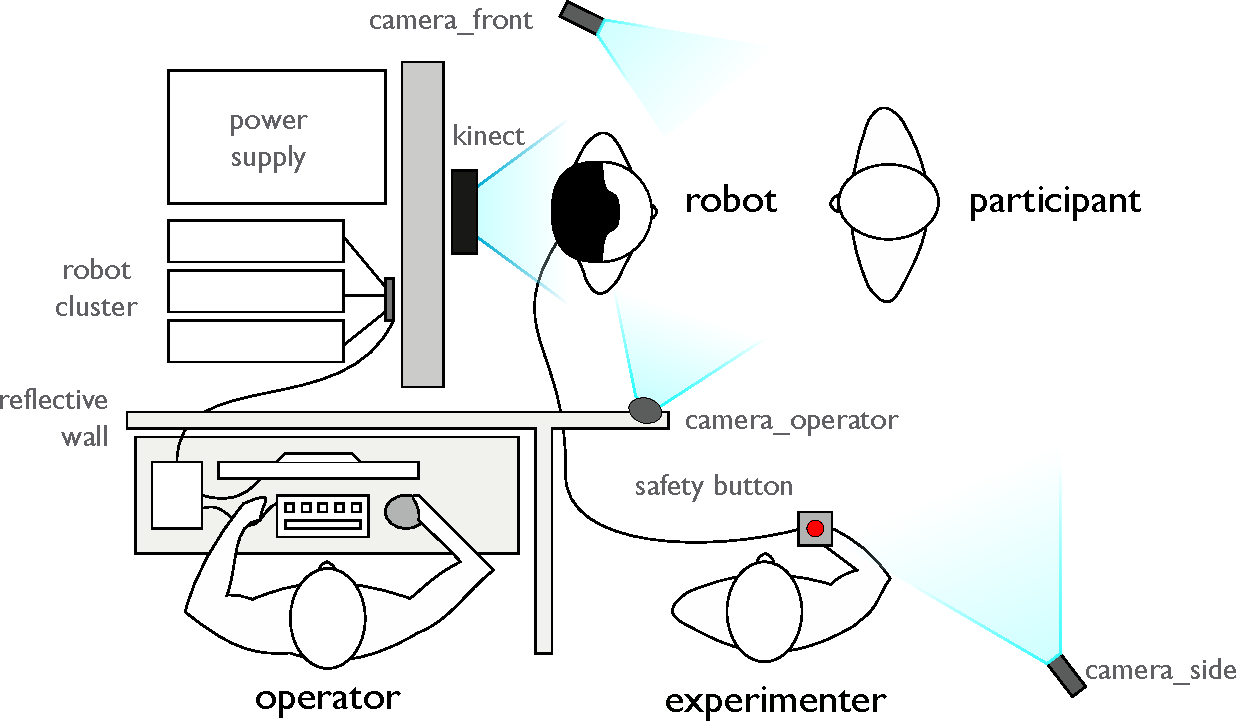
\includegraphics[width=0.7\hsize]{Serena/figures/expe-setting.pdf}
	}
	\caption{The experimental setup. The participant is standing in front of the robot iCub; their interaction is recorded by a Kinect, two standard HD cameras (front and side view of the scene). The experimenter monitors the interaction from the side, not too far but close enough to be able to push the safety button and intervene in case of emergencies. The operator is hidden behind a wall, and he controls the robot monitoring the interaction through a webcam placed over the robot. The power supply and cluster of the robot are hidden behind a cabinet.}
	\label{fig:setup}
\end{figure*}

The experimental setup was organized as depicted in Figure \ref{fig:setup}. 
The robot was standing on a fixed pole, so that it could not fall.
The robot was semi-autonomous, i.e., it was controlled by an operator hidden behind 
a reflective wall (a plastic divider with reflective surface), built  
to prevent the participants to see the operator and the experimenter, while giving the experimenter the possibility to monitor the interaction and intervene promptly in case of problems\footnote{This was done as a safety measure. However, nothing happened during the experiments: the experimenter never had to push the safety button, and she never had to stop the physical interaction between the robot and the subject.}. 

Two cameras were recording the participants, as shown in Figure \ref{fig:setup}. 
One camera was placed behind the robot on its left side, in such a way to observe the human face and upper-body during the close interaction with the robot, while the other one was placed laterally to take the scene as a whole.


The colored rolls used for the assembly task are shown in Figure \ref{fig:rolls}.

\begin{figure}[ht!]
\centering
{
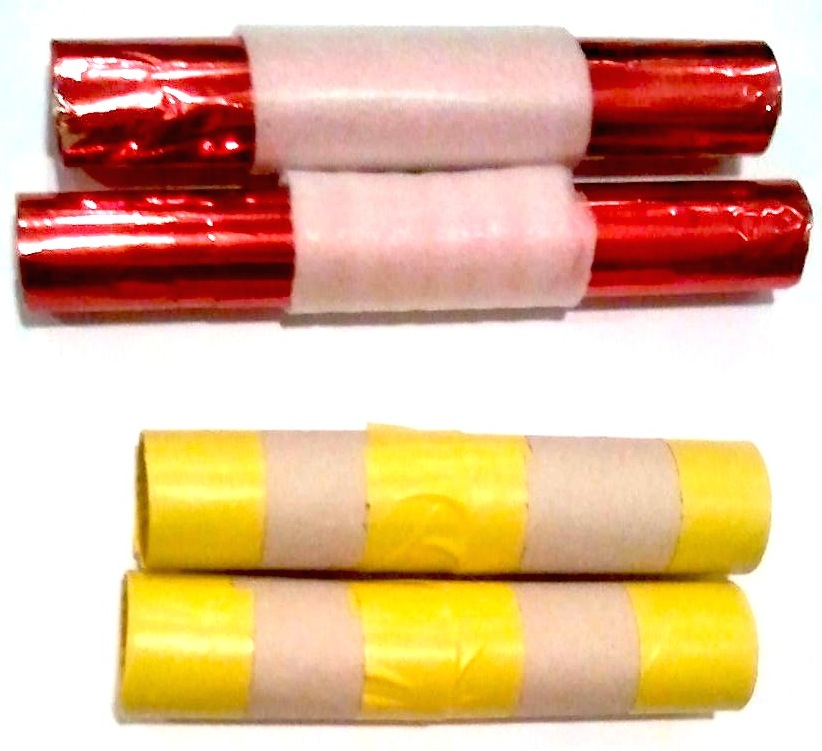
\includegraphics[width=0.4\hsize]{Serena/figures/tubes.jpg}
}
\caption{Colored paper rolls used in the assembly task.}
\label{fig:rolls}
\end{figure}



The experiments were carried out with the humanoid robot iCub \cite{icub2013}. The robot is approximately 104 cm high, weights about 24 kg, and has the shape of a 4 years old child. 


To facilitate the control of the robot by the operator, we developed a graphical user interface (GUI) to quickly send high-level commands to the robot in a wizard-of-Oz mode (WoZ). 
The operator was constantly monitoring the status of the robot, and could intervene to send high-level or low-level commands to the robot, in prompt response to unexpected actions or requests of the participants, using a dedicated graphical interface (see Appendix \ref{appendix:GUI}).
%More details on the GUI and some screenshots are reported in Appendix \ref{appendix:GUI}.

The robot was always controlled in impedance \cite{idyn2012}, to make it compliant in case people would touch it accidentally or intentionally before the construction task. 
When people had to physically manipulate the robot to move its arms and accomplish the task, the operator was switching the robot into a zero-torque control mode that allowed the arms to be driven lightly by the participants. 
%Tactile and force/torque sensors measurements were used to compute precisely the external forces applied by the humans and make the robot move its arms accordingly \cite{idyn2012}. 
For safety issues, the operator could stop the robot motion at any time simply switching the robot to position control, and at the same time the experimenter monitored the whole interaction 
%(during physical contact and without) 
and was able to intervene and stop the robot in case of urgency at any time using the robot safety button. 
Facial expressions and speech were enabled (more details in Appendix \ref{appendix:GUI}).
% The robot was able to say few simple sentences, such as ``yes'', ``no'', ``thank you'' (more details in Appendix\ref{appendix:GUI}). As for the facial expressions, 
The robot always assumed the same neutral/positive expressions, to avoid confusing the participant or suggest an underlying 
%that the participant actions could influence an eventual 
robot ``emotional status''.




%-------------------------------------------------
\subsection{Participants} %OK

Prospective participants were recruited through a generic announcement for HRI studies, diffused on a mailing-list. 
Participants that volunteered in the study received a 10 euros voucher as a symbolic reimbursement for travel expenses. They signed an informed consent form to partake in the study and granted us the use of their recorded data and videos.
N=56 voluntary healthy adults took part in this study: 37 women, 19 men, aged 19 to 65 (mean=36.95, $\sigma$=14.32). The participants were all native French speakers.



%-------------------------------------------------
\subsection{Experimental procedure}\label{section:protocol}


After volunteering to take part in the experiment, the participants received an ID number to preserve anonymity during the study. 
The personality traits of the participants were retrieved by questionnaires that were filled up through an online web form two weeks before doing the experiment, to avoid influences of the questions on their behavior.

The day of the experiment, participants were welcomed by the researcher and informed about the overall procedure before signing an informed consent form granting us the use of all the recorded data for research purposes.

Before the experiment, the participants had to watch a short video presenting the iCub, its body parts and some of its basic movements\footnote{It is a dissemination video from IIT showing the iCub, available on Youtube: {http://youtu.be/ZcTwO2dpX8A}.}. The video did not provide any information about the experiments. It was instrumental to make sure that the participants had a uniform prior knowledge of the robot appearance (some participants may have seen the robot before on the media).


After the video, each participant was equipped with a Lavalier microphone to ensure a clear speech data collection, then was introduced to the robot.
The experimenter did not present the experimental setup (e.g., show the location of the cameras) except showing the robot, and she did not provide any specific instruction to the participants about what to do or say and how to behave with the robot. 
Most importantly, she did not say anything about the 
fact that the robot was not fully autonomous:
%way the robot was controlled: 
since the operator was hidden behind a wall, mixed with other students of the lab, the participant had no cue that the robot was controlled by someone else\footnote{In the post-experiment interview, we asked the participants if they thought or had the impression that the robot was controlled by someone: all the participants thought that the robot was fully autonomous.}.
The robot was in a standing position, gently waving the hands and looking upright, while holding a colored toy in its right hand. 
%It was not speaking. 
Once the participants were standing and looking in front of the robot, they were free to do whatever they wanted: talk to the robot, touch it, and so on. 

%The experimenter then proposed to start the assembly task.
The experimenter explained that the goal of the task was to create an object in collaboration with the robot.
To create the object, they simply had to assemble two paper rolls and fix them with some tape.
The participant could grab the robot arms to demonstrate the bi-manual movement necessary to align the two rolls, as shown in Figure \ref{fig:task}. 

As the task required a physical interaction with the robot, for safety reasons the experimenter had to provide a short demonstration to show the participant how to grab the robot arms in a safe manner and how to ``move'' the robot arms by guidance to teach the robot a desired movement\footnote{The demonstration was also part of the safety measures required by the Ethics Committee to approve our protocol.}.
This demonstration was necessary to make sure that the participants would grab the robot forearm on the cover parts covered by the skin, for their own security and to prevent damaging of cables and robot hands (see Figure \ref{fig:contacts}).
All the participants received the identical demonstration. 
To show a movement to the robot, the experimenter gently grasped the robot forearms touching the skin and saying ``\textit{Be compliant}''. The robot operator then switched the control mode of the robot arms to zero-torque control, so that the experimenter could gently move the arms. To make the arms hold the position, the experimenter said ``\textit{Hold on}''. The operator then switched the control mode of the arms to impedance position control\footnote{The operator could switch the control mode without the need of the verbal command, since he had a direct visibility of the interaction zone in front of the robot through an additional camera that was centered on the workspace in front of the robot (see Figure \ref{fig:setup}).}. 

The short demonstration was necessary for safety reasons, because the participants were not robotics experts.
The experimenter precised that the demonstration was not to be used as a template on how to perform the task with the robot, as neither the task nor the interaction were scripted and the robot would follow the participant's guidance and commands. 


To accomplish the assembly task, the experimenter precised that it was necessary to explain  to the robot how to realize the assembly step by step, even if no scripted procedure was provided. No explicit instructions were given to the participants on how to explain the procedure to the robot.

We remark that the interaction between participant and robot was not scripted, and our aim was to let it be as much as spontaneous as possible for a first human-humanoid interaction.

The experimenter then gave the participants the first two colored paper rolls and invited the participant to start the assembly task with the robot; the task had to be repeated three times with three pairs of paper rolls, so as to build three objects. The paper rolls and the tape were conveniently placed on a table next to the participants.
The participant was free to start at his/her own convenience, and to make each trial last how much he/she wanted to.
Some paper rolls used in the experiments are shown in Figure \ref{fig:rolls}.


\begin{figure*}[ht!]
\centering
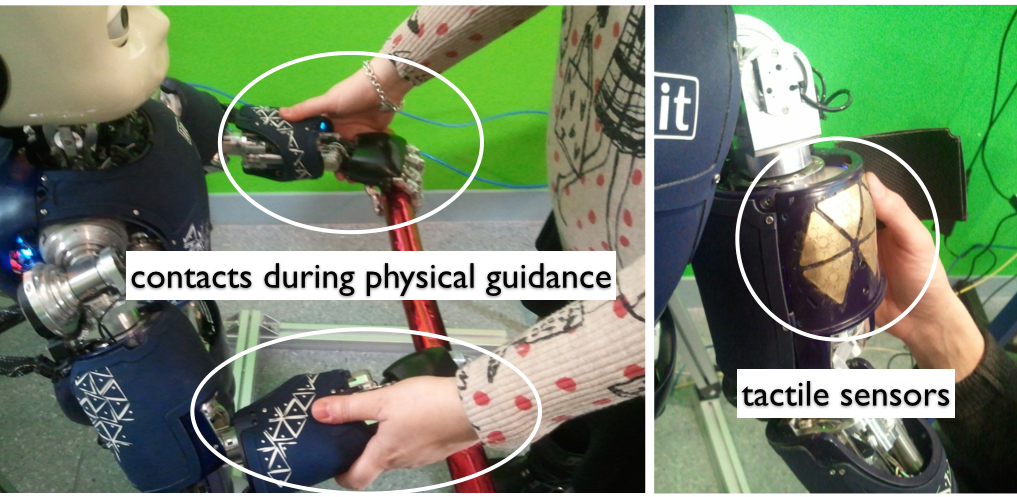
\includegraphics[width=0.7\hsize]{Serena/figures/contacts_guidance.png}
\caption{Demonstration on how to safely grab the robot arms for kinesthetic teaching in the assembly task: the hands of the experimenter grasp the robot forearms on a part covered by the skin. On the left, the distributed tactile sensors underneath the cover.}
\label{fig:contacts}
\end{figure*}


\begin{figure*}[ht!]
\centering
%\includegraphics[width=0.95\hsize]{figures/figure_2.jpg}
\includegraphics[width=0.7\hsize]{Serena/figures/construction_phases_bar.jpg}
\caption{Demonstration of the assembly task: 1) the participant asks the robot to grasp the two cylinders; 2) the participant grabs the robot arms and demonstrates how to move them to align the two cylinders; 3) the participant fixes the cylinders with some tape while the robot is holding them; 4) the participant retrieves the assembled object from the robot. }
\label{fig:task}
\end{figure*}

Once the participants finished the assembly task, repeated three times, the experimenter led the participant back to a computer to make him/her fill a post-experiment questionnaire and then get feedback and impressions through a short interview.

\begin{figure*}[ht!]
\centering
{
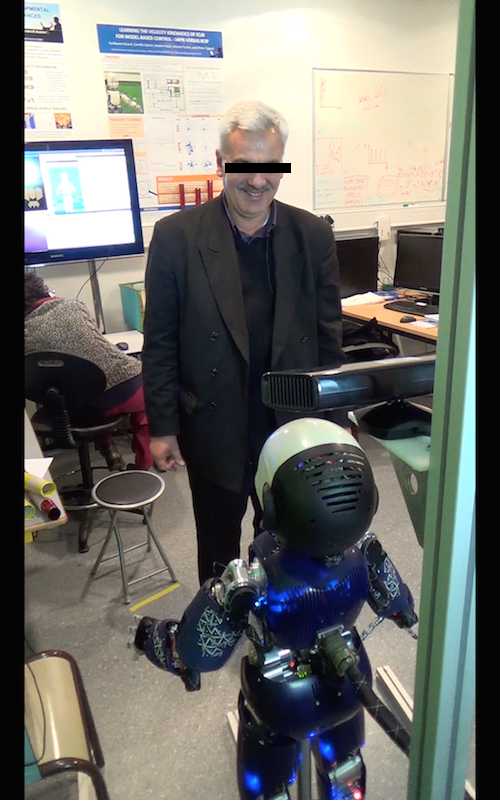
\includegraphics[width=0.2\hsize]{Serena/figures/manipulation_screenshots/people_gazing/gaze1.png}
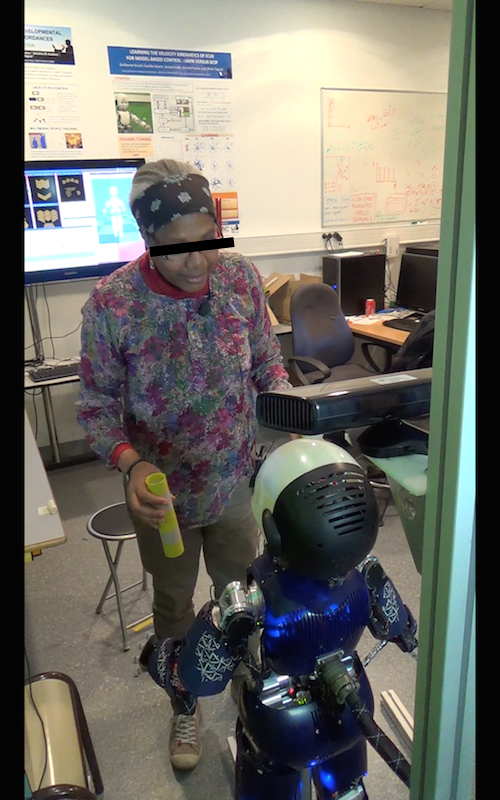
\includegraphics[width=0.2\hsize]{Serena/figures/manipulation_screenshots/people_gazing/gaze2.png}
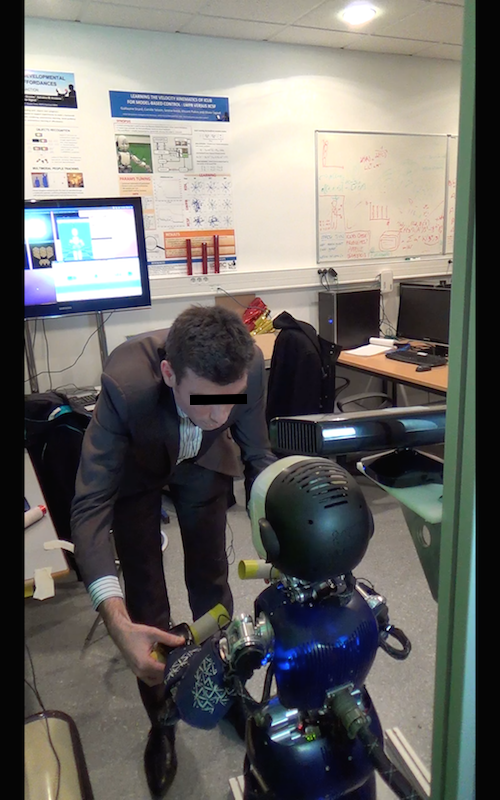
\includegraphics[width=0.2\hsize]{Serena/figures/manipulation_screenshots/people_gazing/gaze3.png}
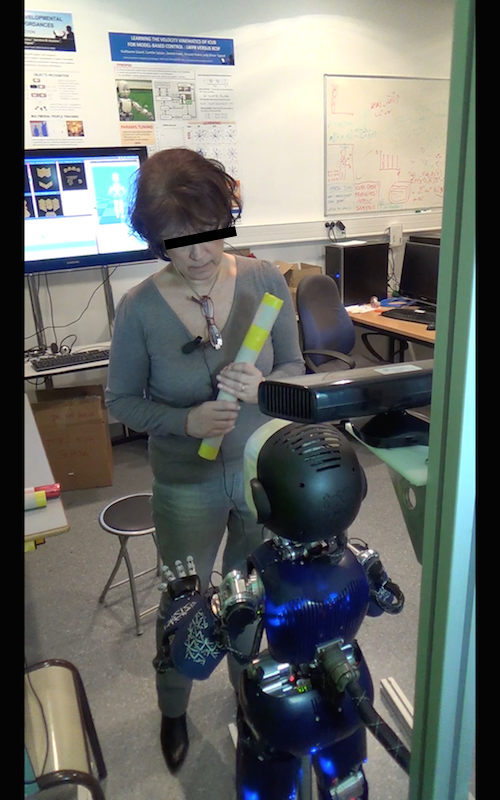
\includegraphics[width=0.2\hsize]{Serena/figures/manipulation_screenshots/people_gazing/gaze5.png}
}

\caption{Some participants gazing at the robot face. From left to right: when the participant meets the robot, handing the cylinders, during the alignment of cylinders, and when the object is built.}
\label{fig:shotsgaze}
\end{figure*}

\begin{figure*}[ht!]
\centering
{
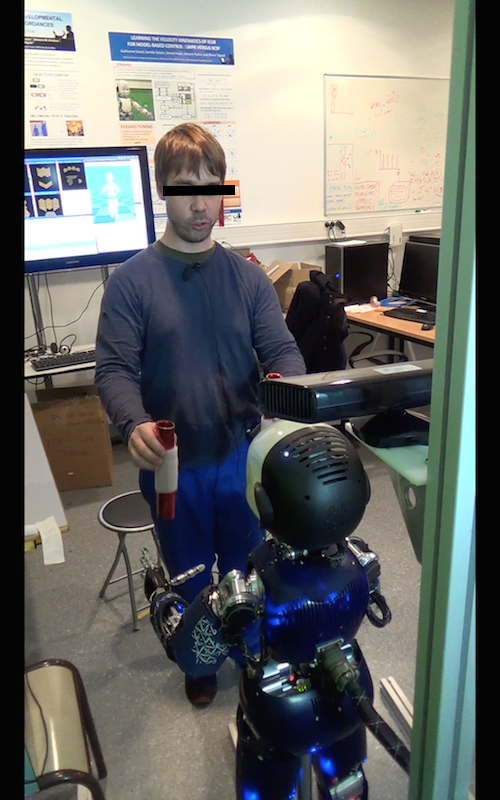
\includegraphics[width=0.23\hsize]{Serena/figures/manipulation_screenshots/people_contact/contact_guy_1.png}
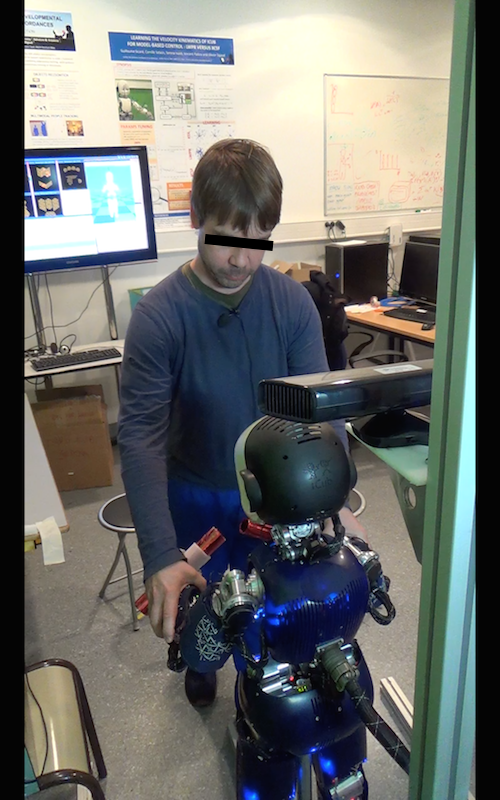
\includegraphics[width=0.23\hsize]{Serena/figures/manipulation_screenshots/people_contact/contact_guy_2.png}
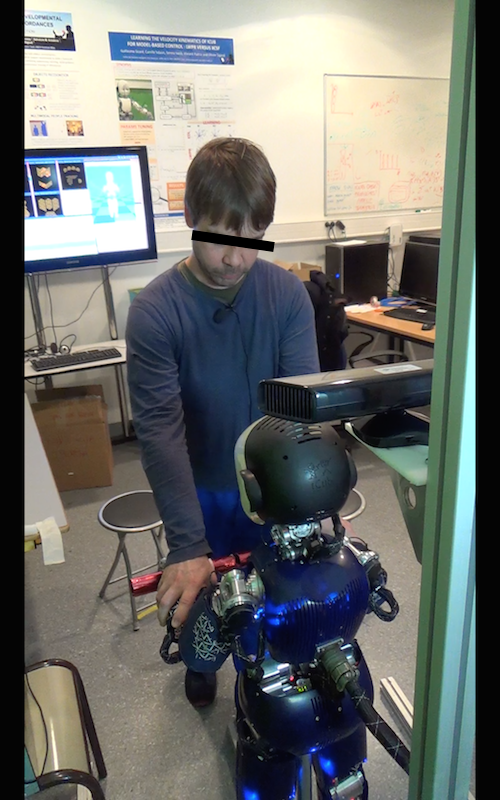
\includegraphics[width=0.23\hsize]{Serena/figures/manipulation_screenshots/people_contact/contact_guy_3.png}

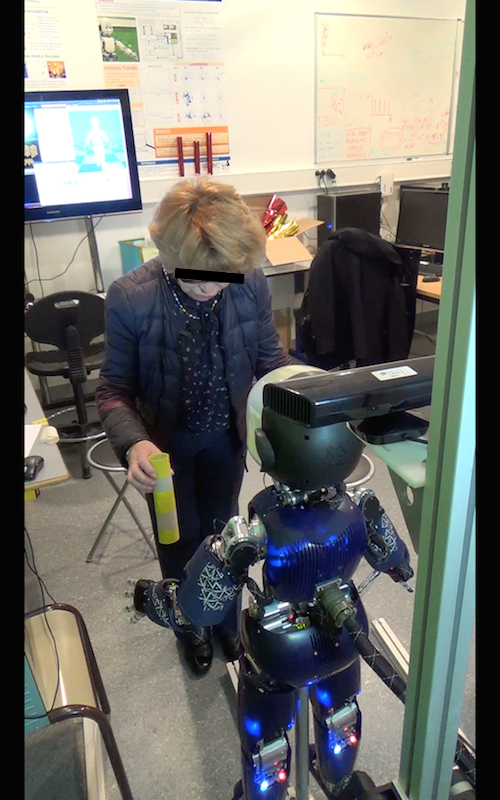
\includegraphics[width=0.23\hsize]{Serena/figures/manipulation_screenshots/people_contact/contact_vecchia_1.png}
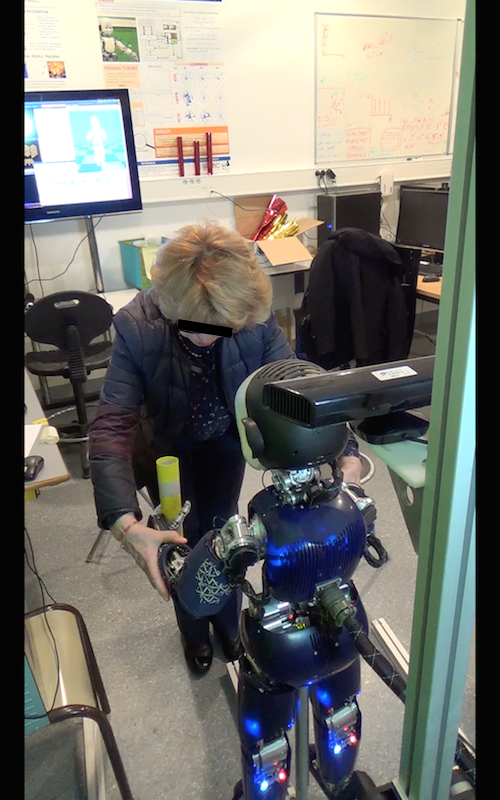
\includegraphics[width=0.23\hsize]{Serena/figures/manipulation_screenshots/people_contact/contact_vecchia_2.png}
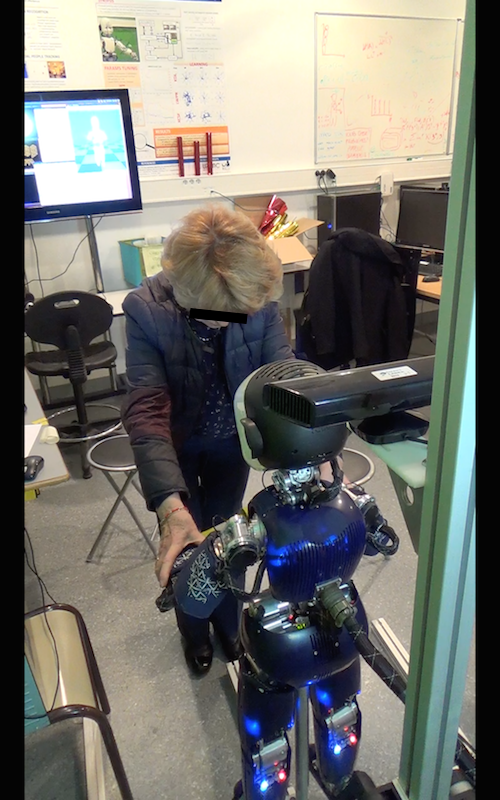
\includegraphics[width=0.23\hsize]{Serena/figures/manipulation_screenshots/people_contact/contact_vecchia_3.png}
}

\caption{Some participants performing the assembly task (screenshots from the front camera). The three images show the participants giving the cylinders to the robot (left), grabbing the robot arms (center) then moving the arms to align the cylinders (right).}
\label{fig:shotscontact}
\end{figure*}

\begin{figure*}
\centering
{
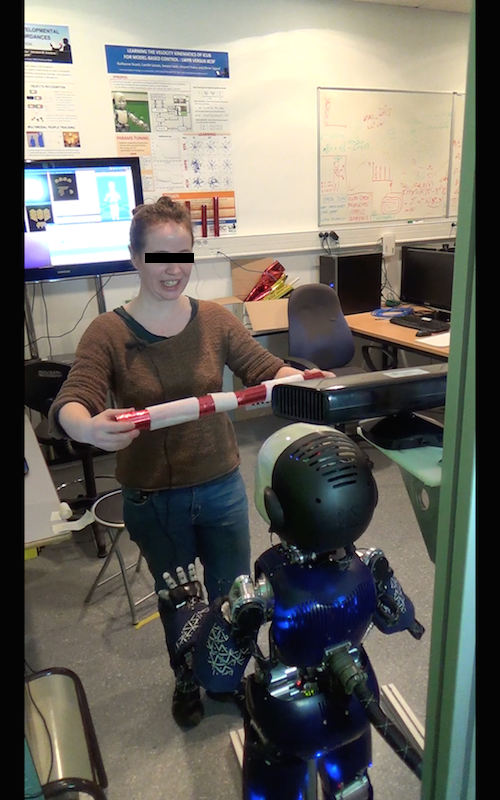
\includegraphics[width=0.2\hsize]{Serena/figures/manipulation_screenshots/people_show_result_after/finished1.png}
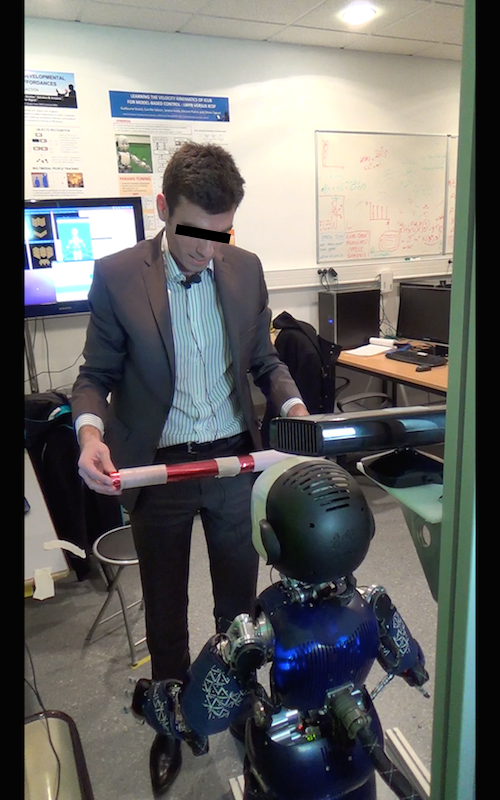
\includegraphics[width=0.2\hsize]{Serena/figures/manipulation_screenshots/people_show_result_after/finished2.png}
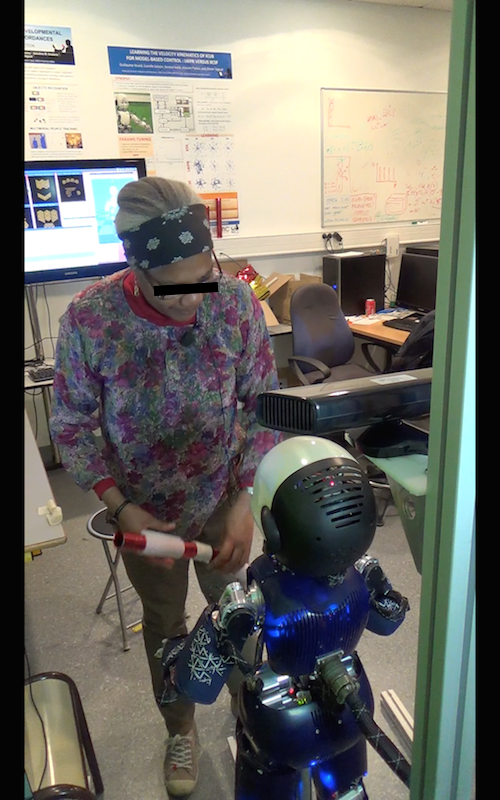
\includegraphics[width=0.2\hsize]{Serena/figures/manipulation_screenshots/people_show_result_after/finished3.png}
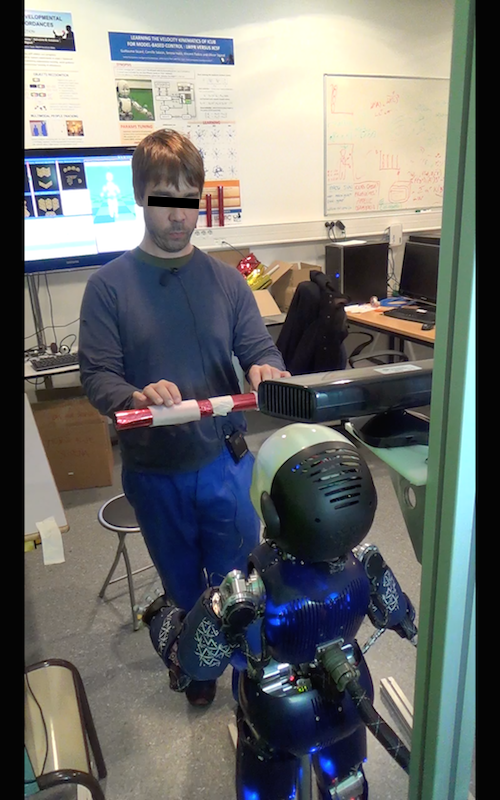
\includegraphics[width=0.2\hsize]{Serena/figures/manipulation_screenshots/people_show_result_after/finished4.png}
}
\caption{Some participants showing the final object to the robot, after the collaborative assembly.}
\label{fig:shotsfinished}
\end{figure*}


\begin{table*}
\caption*{\textbf{Post-experimental questionnaire for human-humanoid collaborative tasks with physical interaction}}
%\textbf{Post-experimental questionnaire for human-humanoid collaborative tasks with physical interaction}
\resizebox{\textwidth}{!}{%
\begin{tabular}{|p{12cm}|p{3.5cm}|}
\hline
 Questionnaire Item & Subjective evaluation (score mean $\pm$ stdev) \\
 \hline
 \hline
\multicolumn{2}{|l|}{\textbf{Questions related to the task}} \\
\hline            
 The assembly task was easy to do. & 5.49 $\pm$ 1.39\\
 \textbf{The assembly task was interesting to do.}& \textbf{5.75 $\pm$ 1.61}\\
 Someday I could work with this robot to build something of interest.& 5.03 $\pm$ 1.67\\
\textbf{Someday I could work with a robot to build something of interest.}& \textbf{5.87 $\pm$ 1.07}\\
\hline
\multicolumn{2}{|l|}{\textbf{Questions related to the physical interaction (e.g., touching the robot)}} \\
\hline  
\textbf{I was worried to must touch the robot to assembly the objects with it.} & \textbf{2.13 $\pm$ 1.46}\\
\textbf{I was afraid to touch the hands of the robot.} & \textbf{2.36 $\pm$ 1.72} \\
 I was afraid to damage the robot. &	3.57 $\pm$ 1.91 \\
\textbf{The robot does not look dangerous.}& \textbf{6.00 $\pm$ 1.57}\\
\textbf{The robot is not threatening.}& \textbf{6.02 $\pm$ 1.49}\\
\hline
\multicolumn{2}{|l|}{\textbf{Questions related to the cognitive/social interaction}} \\
\hline 
 During the assembly, I would have preferred that the robot tells me what it thinks, if it understands well. & 5.19 $\pm$ 1.61 \\
 The robot understood what I explained to it.&	 5.38 $\pm$ 1.39\\
 The robot should be more reactive.& 4.65 $\pm$ 1.56\\
  The robot was nice. & 5.49 $\pm$ 1.37\\
\hline
\multicolumn{2}{|l|}{\textbf{Questions related to the robot features}} \\
\hline 
 The robot moves its head too slowly. & 3.32 $\pm$ 1.41\\
 The robot moves its arms too slowly. & 3.55 $\pm$ 1.33\\
\textbf{The facial expressions of the robot trouble me.}& \textbf{2.03 $\pm$ 1.29}\\
 The voice of the robot is pleasant.& 4.51 $\pm$ 1.84\\
\hline
\end{tabular}}
\caption{The scores of the post-experimental questionnaire for evaluating the perception and interaction with the iCub in the assembly task of this work. The second column reports the mean and standard deviation of the scores attributed on a 7-items Likert scale (from 1=totally disagree to 7=totally agree) by the N=56 participants in this study. We highlight in bold the questions where the score is close to the maximum or the minimum score.}
\label{table:postexperimentquestionnairescores}
\end{table*}


%-------------------------------------------------
\subsection{Data analysis}

The questionnaires scores for extroversion and NARS were computed according to their authors' recommendation. 

The audio-video recordings were analyzed with CowLog software \cite{CowLog2009}. 
 Six events were annotated: beginning of the interaction, end of the interaction, beginning of a gaze by the participant towards the robot's face or hands (i.e., the contact area), end of that gaze, beginning of an utterance addressed to the robot, end of that utterance. 
The gaze direction was approximated by the head orientation, as it is often done in literature \cite{ivaldi2014frontiers,Ba2009}. 
We considered two consecutive utterances whenever there was a pause of at least 500ms. 

We computed from the events' timestamps the following six dependent measures: frequency and duration of gaze towards the robot's face, frequency and duration of gaze towards the robot's hands, frequency and duration of utterances addressed to the robot. 
These indicators were normalized by the total duration of the interaction, to take into account inter-individual variability in terms of task duration.

We used Pearson's correlation to test of correlation of the extroversion and attitude towards robots on the frequency and duration of gaze and utterances\footnote{Correlation is frequently used to study the link between personality and behavior, as discussed in \cite{LaFrance2004}, a survey on the link between extroversion and behavior where all the cited studies use correlations to test their hypothesis.}.




%=================================
%=================================
\section{Results}

The average time to complete the task was 246.10s ($\sigma$= 75.45). 
On average, the participants talked to the robot for 69.92s ($\sigma$=38.38), addressing to it 57.54 utterances ($\sigma$= 25.65); they looked at the robot's face for 42.55s ($\sigma$=29.25), gazing at the face of the robot 12.13 ($\sigma$=6.57) times; they looked at the robot's hands for 162.46s ($\sigma$=57.14), gazing at the hands 11.30 ($\sigma$=5.70) times.


\subsection{On the individual factors}
To ensure that the two questionnaires capture two different individual factors, we computed the correlation between the scores of extroversion and negative attitude towards robot obtained by our population of participants.
We did not find a significant correlation between the two ($r^2$=-0.213; p=N.S.), neither between extroversion and  
each of the three sub-scales: negative attitude towards interaction with robots ($r^2$=-0.156; p=N.S.), negative attitude towards social influence of robots ($r^2$= -0.156; p=N.S.), and negative attitude towards emotions during the course of interactions with robots ($r^2$=-0.254; p=N.S.). 

These results seem to indicate that both questionnaires represent a fair valuation of the different individual traits of the participants. 


\subsection{Relation of extroversion to gaze and speech}\label{sec:extro}

The participants' average extroversion score was 111.77 ($\sigma$=22.86; min=61, max=160), which is, according to \cite{NEOPIR1998}, a neutral level of extroversion\footnote{According to the NEO-PIR, a participant obtaining a score bigger than 137 is considered extrovert, while one with a score below 80 is introvert.}. 

Table~\ref{table:extroversion} reports the Pearson's correlation between the extroversion score of the participants and their gaze and utterance frequency and duration. 
The extroversion score is significantly and positively correlated to the frequency and duration of utterances (see Table~\ref{table:extroversion}). This can also be seen in the scatter graphs in Figure~\ref{fig:extroversionutterance}.
Conversely, the results indicate that extroversion does not influence the gaze signal, as there is no significant correlation between the personality trait and the gaze frequency or the duration of gaze.

To summarize, the more an individual is extrovert, the more he/she will tend to talk to the robot during an assembly task to provide instructions. 
On the contrary, an individual with a high score of extroversion will not look at the robot's face or hands more than individuals with lower scores.

Therefore, with reference to the research hypothesis expressed in Section~\ref{sec:hypotheses}, we confirm Hypothesis 1, and reject Hypothesis 2.


\begin{table*}
\centering
\begin{tabular}{|p{6cm}|p{4.5cm}|}
\hline
Variable & \textbf{Extroversion score}  \\
\hline
\hline
Gaze towards face frequency  & $r^2$= -0.13 ; p=0.927 (N.S.)  \\
%\hline
Gaze towards face duration  & $r^2$= 0.098 ; p=0.471 (N.S.) \\
\hline
Gaze towards hands frequency  & $r^2$= 0.058 ; p=0.671 (N.S.)  \\
%\hline
Gaze towards hands duration  & $r^2$= 0.215 ; p=0.875 (N.S.) \\
\hline
\textbf{Utterance frequency}  &	\textbf{$\mathbf{r^2}$= 0.318 ; p=0.017 ($\mathbf{<}$0.05)}  \\
%\hline
\textbf{Utterance duration} &	\textbf{$\mathbf{r^2}$= 0.321 ; p=0.016 ($\mathbf{<}$0.05)}  \\
\hline
\end{tabular}
\caption{Correlation between the participants' extroversion score (computed by NEO-PI-R \cite{NEOPIR1998}) and their gaze and utterance frequency (number/s) and duration (normalized ratio) during the assembly task.}
\label{table:extroversion}
\end{table*}

\begin{figure}[ht!]
\centering
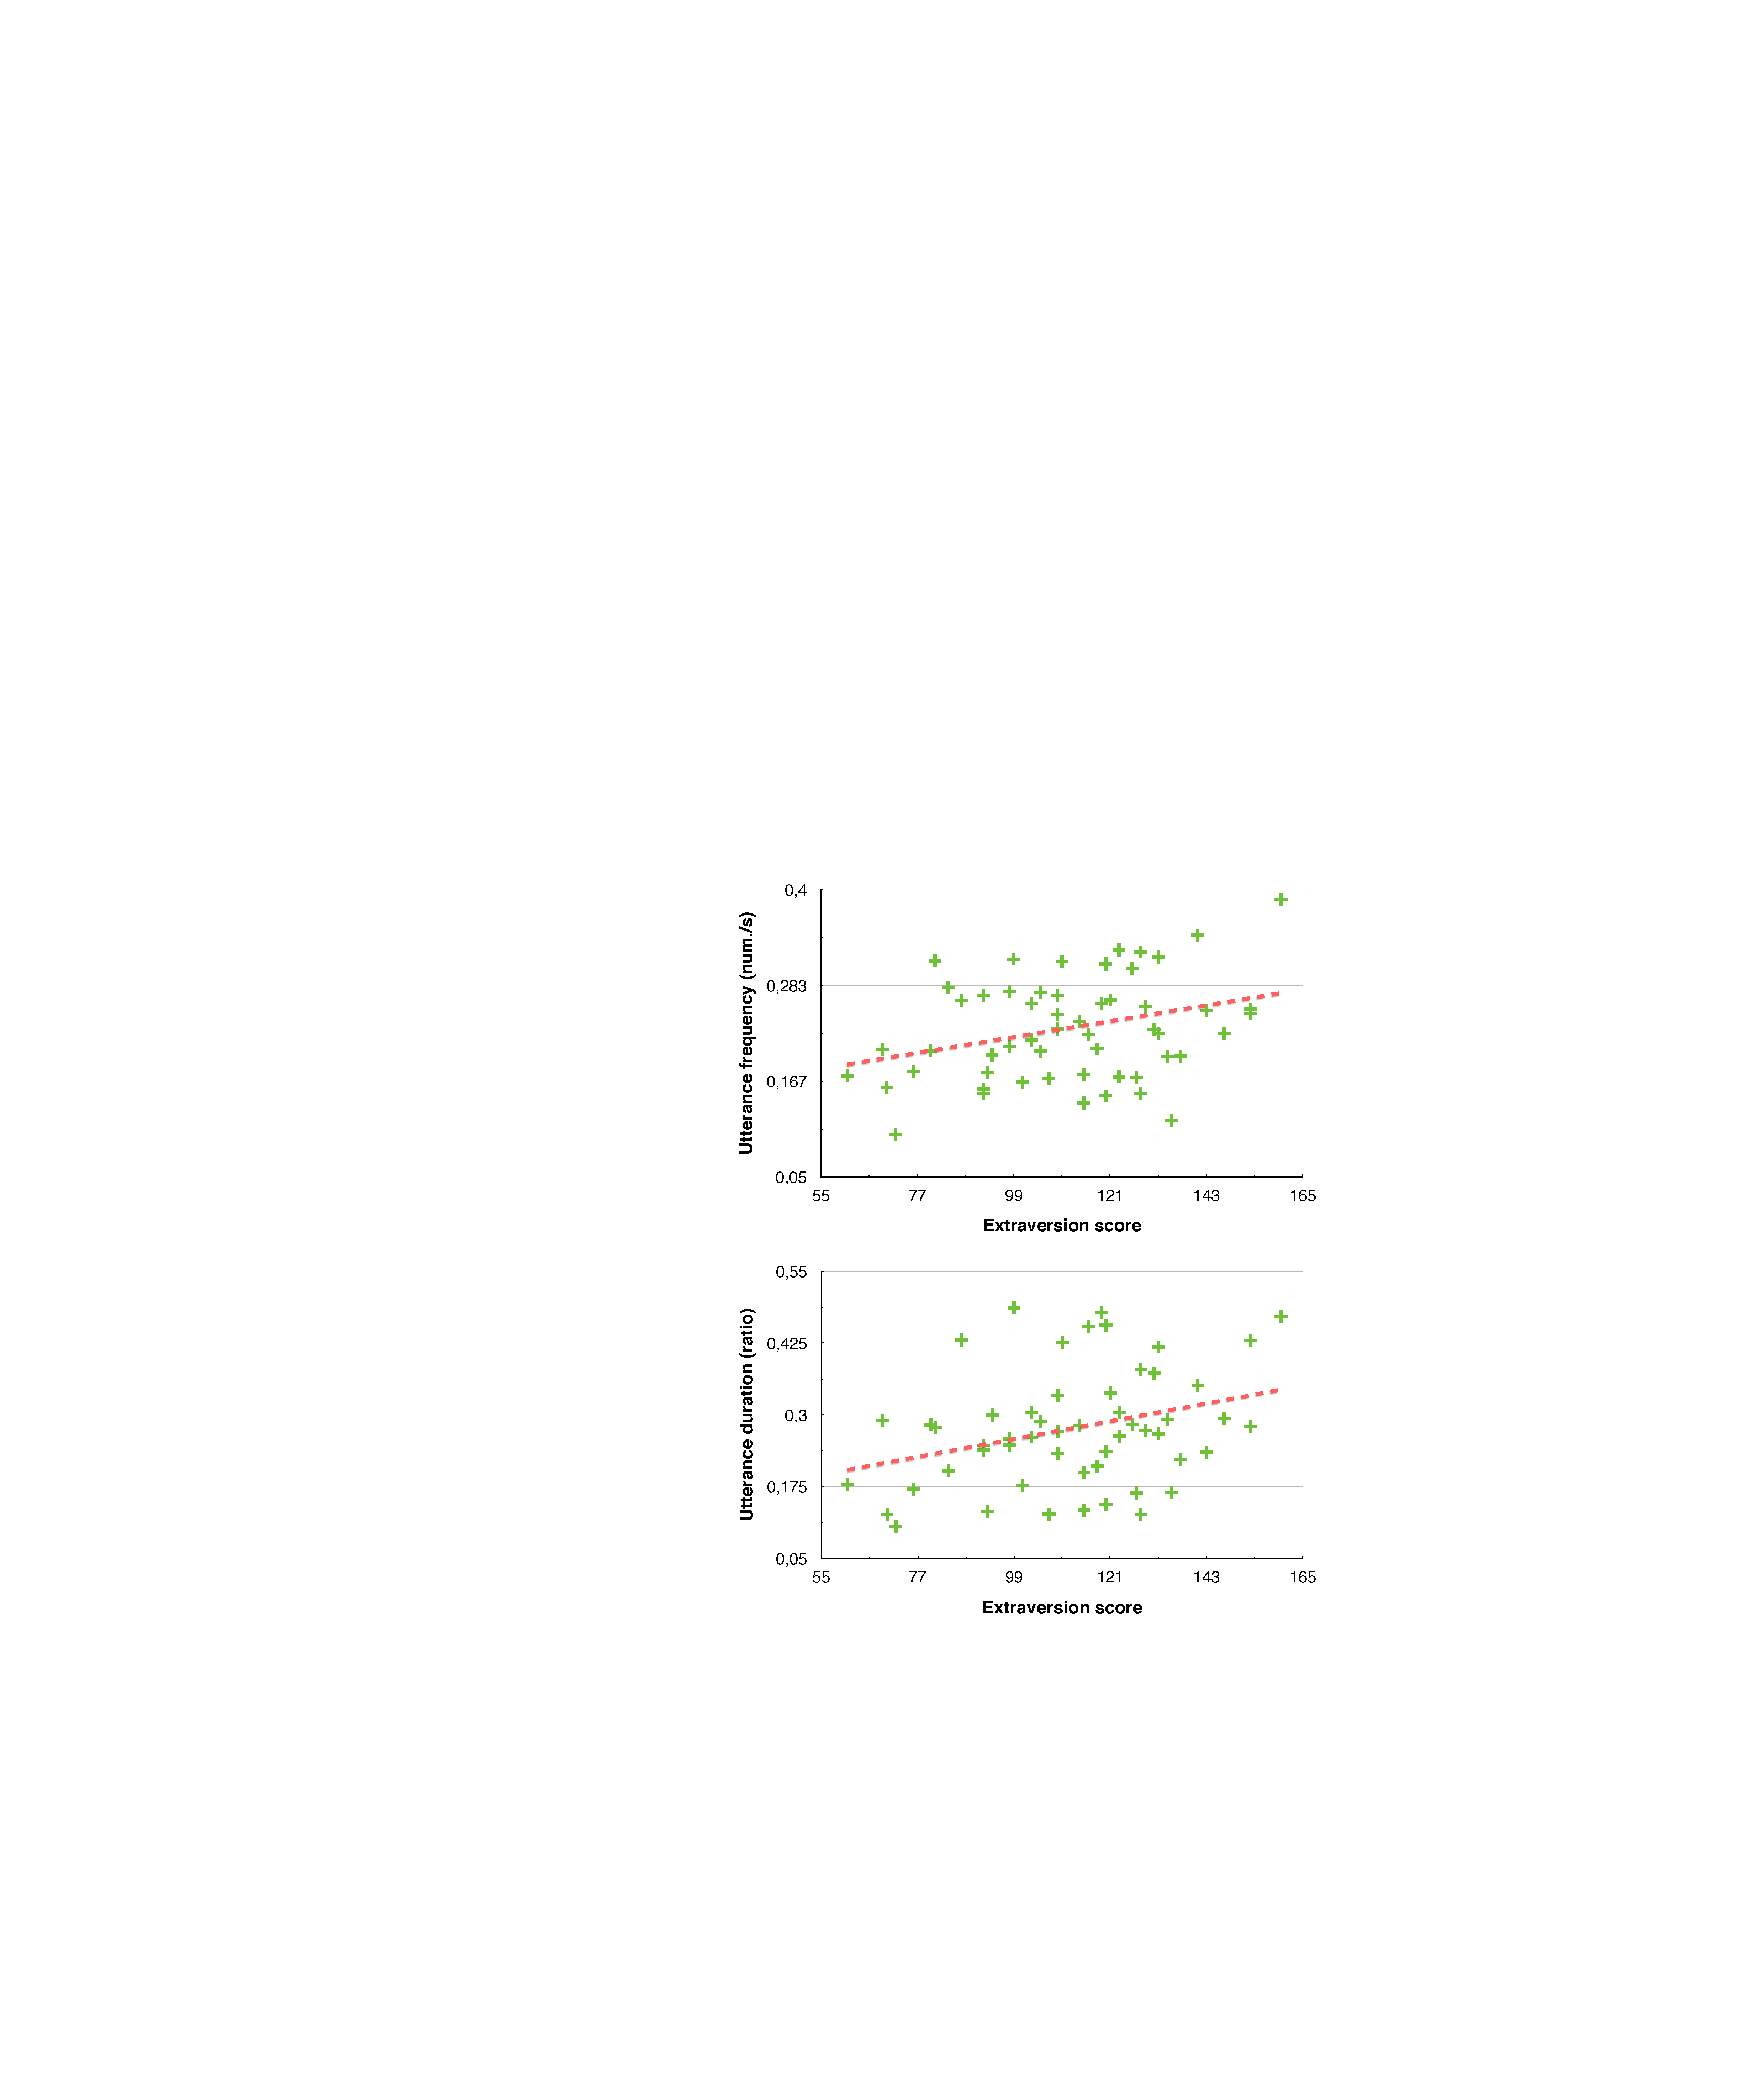
\includegraphics[width=0.5\hsize]{Serena/figures/plots_extraversion_utterance_3.pdf}
\caption{Scatter graphs showing the frequency (number/seconds) and duration (normalized ratio) of utterances of the participants (N=56), in function of their extroversion score.}
\label{fig:extroversionutterance}
\end{figure}


\subsection{Relation of negative attitude towards robots to gaze and speech}\label{sec:nars}

The participants' average score for the negative attitude was 45.55 ($\sigma$=12.74; min=20, max=77), which is a neutral value for the attitude towards robots\footnote{According to the NARS, a score over 65 is a sign of negative attitude towards robots, while a score below 35 indicates a rather positive attitude towards robots.}. 

Table~\ref{table:nars} reports the Pearson's correlation between the NARS scores of the participants and their gaze and utterance frequency and duration. The results indicate that the negative attitude does not influence the verbal signal, as there is no significant correlation with the utterance frequency or duration. 
There is, however, a partial effect on the gaze signal. Precisely, the negative attitude is significantly and negatively related to the duration of gaze towards the robot's face, and positively related to the duration of gaze towards the robot's hands, as visible in Figure~\ref{fig:narsgaze}. 

To summarize, the more an individual has a negative attitude towards robots, the less he/she will tend to look at the robot's face during an assembly task, and the more he/she will tend to look at the robot's hands (area of physical contact). The gaze frequency, on the contrary, will not change in relation to different positive or negative attitudes. 
Nothing can be concluded regarding the verbal communication: an individual with a more negative attitude towards robots will not speak more or less to the robot than other individuals with a more positive attitude. 

Therefore, with reference to the research hypothesis expressed in Section~\ref{sec:hypotheses}, we reject Hypothesis 3
% and partially reject Hypothesis 4. 
and partially confirm Hypothesis 4 and 5, since the NARS score relates to the gaze duration but not to the gaze frequency.


\begin{table*}
\centering
\begin{tabular}{|p{6cm}|p{8cm}|}
\hline
Variable & \textbf{Negative attitude towards robots score (NARS)} \\
\hline
\hline
Gaze towards face frequency  &  $r^2$= -0.174 ; p=0.201 (N.S.) \\
%\hline
\textbf{Gaze towards face duration}  & \textbf{$\mathbf{r^2}$= -0.331 ; p=0.013 ($\mathbf{<}$0.05)} \\
\hline
Gaze towards hands frequency  &  $r^2$= -0.111 ; p=0.413 (N.S.) \\
%\hline
\textbf{Gaze towards hands duration}  & \textbf{$\mathbf{r^2}$= 0.355 ; p=0.007 ($\mathbf{<}$0.05)} \\
\hline
Utterance frequency  &	$r^2$= -0.137 ; p=0.314 (N.S.) \\
%\hline
Utterance duration  &	$r^2$= 0.033 ; p=0.807 (N.S.) \\
\hline
\end{tabular}
\caption{Correlation between the participants' negative attitude towards robots score (computed by NARS \cite{NARS2006}) and their gaze and utterance frequency (number/seconds) and duration (normalized ratio) during the assembly task.}
\label{table:nars}
\end{table*}

\begin{table*}
\centering
\resizebox{\textwidth}{!}{%
\begin{tabular}{|p{5.5cm}|p{2.9cm}|p{2.9cm}|p{2.9cm}|}
\hline
Variable & \textbf{NARS-S1} & \textbf{NARS-S2} & \textbf{NARS-S3} \\
\hline
\hline
Gaze towards face frequency  & $r^2$=-0.160; p=0.238 (N.S.)	 & $r^2$=-0.215; p=0.111 (N.S.)	& $r^2$=0.009; p=0.947 (N.S.) \\
%\hline
\textbf{Gaze towards face duration}  & \textbf{$\mathbf{r^2}$=-0.311; p=0.020 ($\mathbf{<}$0.05)}	& \textbf{$\mathbf{r^2}$=-0.334; p=0.012 ($\mathbf{<}$0.05)}	& $r^2$=-0.120; p=0.377 (N.S.)\\
\hline
Gaze towards hands frequency  & $r^2$=-0.073; p=0.592	(N.S.) & $r^2$=-0.138; p=0.310	(N.S.) & $r^2$=-0.043; p=0.754 (N.S.)\\
%\hline
\textbf{Gaze towards hands duration}  & \textbf{$\mathbf{r^2}$=0.381; p=0.004 ($\mathbf{<}$0.05)}	& \textbf{$\mathbf{r^2}$=0.334; p=0.012	($\mathbf{<}$0.05)} & $r^2$=0.094; p=0.491 (N.S.)\\
\hline
\textbf{Utterance frequency}  & $r^2$=0.018; p=0.895 (N.S.)	& $r^2$=-0.093; p=0.497	 (N.S.)& \textbf{$\mathbf{r^2}$=-0.323; p=0.015 ($\mathbf{<}$0.05)} \\
%\hline
Utterance duration   &	$r^2$=0.172; p=0.203 (N.S.)	& $r^2$=0.058; p=0.673 (N.S.) &	$r^2$=-0.249; p=0.063 (N.S.) \\
\hline
\end{tabular}}
\caption{Correlation between the scores of the NARS sub-scales (computed as in \cite{NARS2006}) of the participants and their gaze and utterance frequency (number/seconds) and duration (normalized ratio) during the assembly task.}
\label{table:narsspecific}
\end{table*}


\begin{figure}[ht!]
\centering
%\includegraphics[width=0.7\hsize]{Figures/nars_gaze.pdf}
%\includegraphics[width=0.99\hsize]{Figures/plots_nars_gaze.pdf}
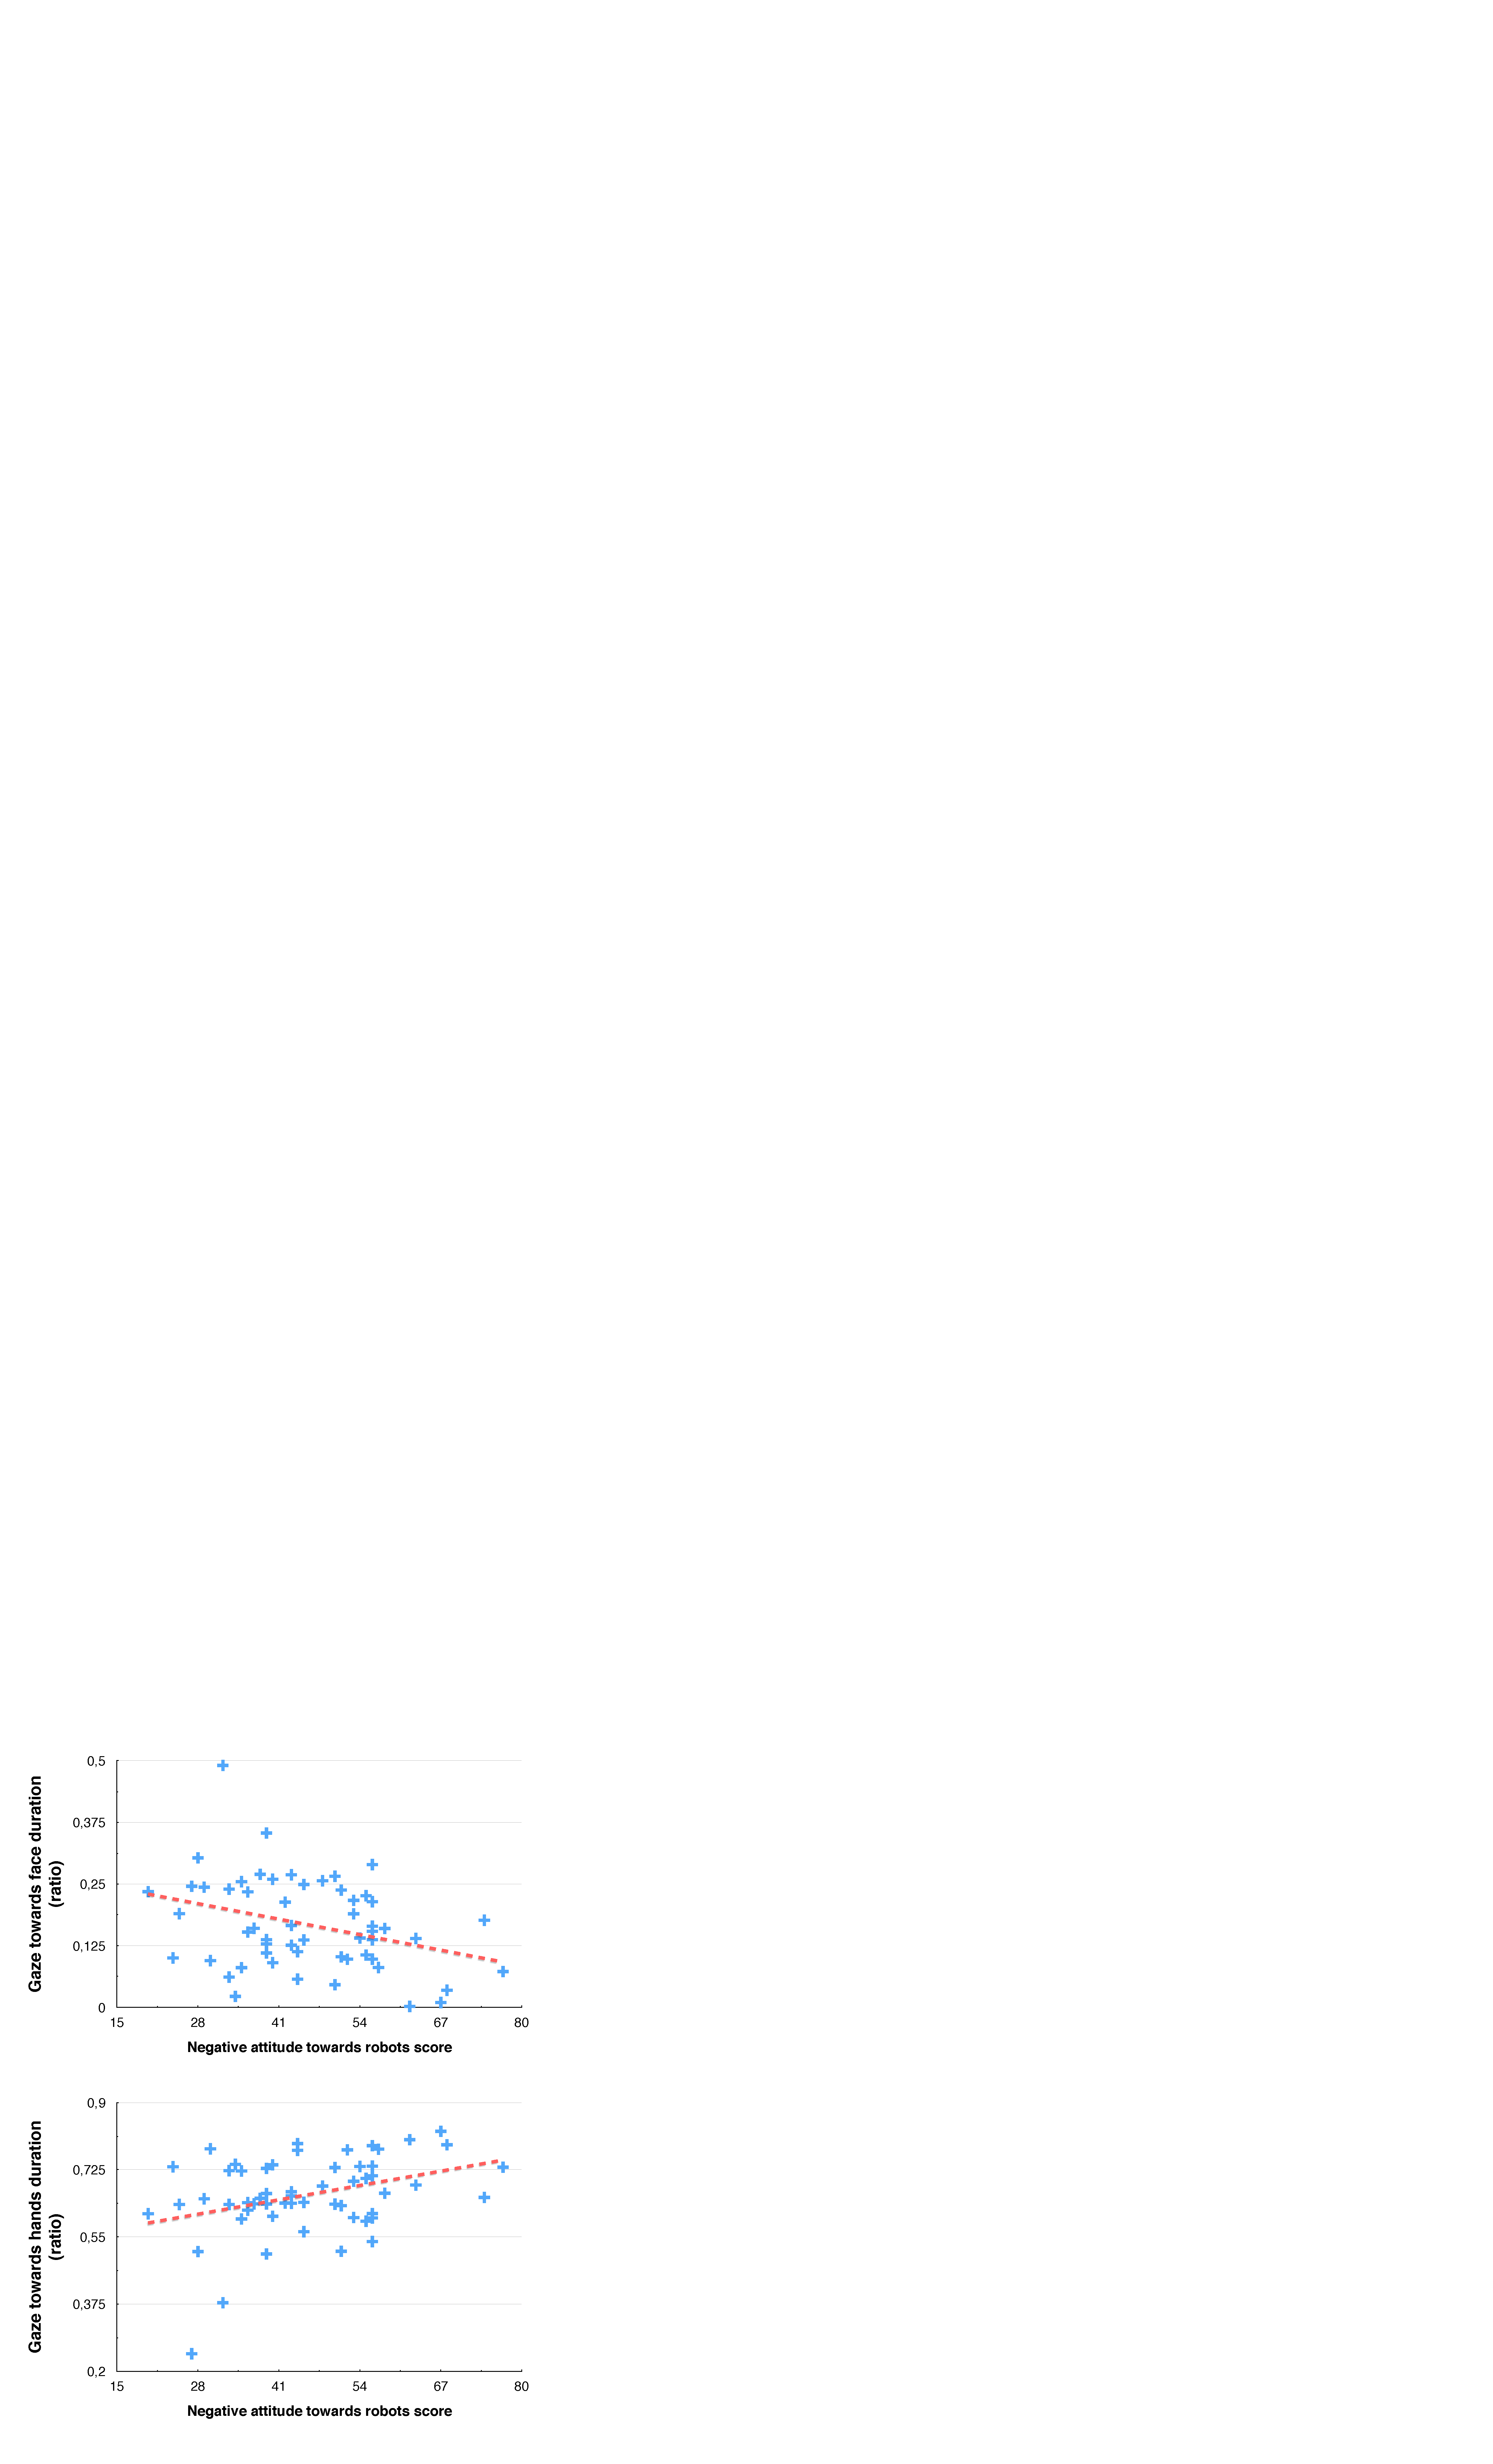
\includegraphics[width=0.5\hsize]{Serena/figures/plots_nars_gaze_3.pdf}
\caption{Scatter graph showing the duration of gaze (normalized ratio) of the participants (N=56) towards the robot hands and face, in function of their NARS score. }
\label{fig:narsgaze}
\end{figure}

As explained in Section~\ref{sec:material}, the NARS questionnaire is based on three sub-scales.
The participants' average scores of negative attitude towards interaction situations (S1), social influence of robots (S2) and emotions during interaction (S3) were respectively 15.18 ($\sigma$=5.83), 18.80 ($\sigma$=5.83) and 11.70 ($\sigma$=3.82), whereas the mean values of the three sub-scales were 24, 20 and 12. 
We performed a thorough investigation of the effect of each of the three sub-scales on gaze and utterances. 
For the gaze signal, we did not find any significant correlation between the sub-scales values and its frequency; however, we found a significant and negative correlation between the gaze duration and S1 ($r^2$=-0.311; \textbf{$p<0.05$}) and S2 ($r^2$=-0.334; \textbf{$p<0.05$}).
For the verbal signal, we did not find any significant correlation between the sub-scales values and the utterance duration, however we found a significant negative correlation between S3 and the utterance frequency ($r^2$=-0.323 ; \textbf{$p<0.05$}).

To summarize, the more people display a negative attitude \textit{in the interaction} (S1) with the robot and are concerned by the \textit{social aspect} (S2) of the interaction, the less they will look at the robot. Conversely, the more people are negative about the \textit{emotions during the interaction} (S3), the less they will talk to the robot.



\subsection{Post-experiment evaluation}

The post-experimental questionnaire for subjective evaluation does not have a score. 
It was designed by the experimenter to get a simple feedback on the user experience, retrieve the global impression and the personal evaluation of the participants on some aspects of the task.
Table \ref{table:postexperimentquestionnairescores} reports on the average score for each item in the questionnaire. We highlighted in bold the most significant questions, which have an average score that is close to the maximum (7) and minimum (1).





\section{Discussion}

%\todo{short discussion of the overall positive feedback}


As discussed in Section \ref{sec:background}, the literature in psychology highlights an effect of personality traits, particularly of the extroversion dimension, on the dynamics of speech and gaze. Likewise, a negative attitude towards robots will influence the time of the verbal response during interactions.
These results induced us to question the reliability of the metrics used for the estimation of the engagement in HRI, classically based on the dynamics of social signals, as their dynamics may be altered by individual factors that are not taken into account in the models of engagement.

In the following we discuss here the results on the correlations between two individual factors (extroversion and negative attitude towards robots) and the dynamics of speech and gaze observed during the human-robot assembly task. We argue about the implications of our study for the HRI community and consider the limits of our study. 


%\section{Effect of extroversion}
\subsection{Extroversion \& social signals}
As detailed in Section~\ref{sec:extro}, we found that there is a positive and significant correlation between the extroversion score and the frequency and duration of utterances.
The more the individual is extrovert, the more often and longer he/she will tend to address the robot during the interaction. 
This result is consistent with observations of human-human interactions, showing that introverts tend to talk less than extroverts \cite{Scherer1981}. 
Conversely, we did not find a significant correlation between the extroversion and the gaze frequency or duration. This finding is partially contrary to what has been observed in \cite{Iizuka1992}, where the author found a relationship between the extroversion and the amount of time spent gazing while listening. However, the author also observed that the gaze duration was not related to extroversion when people were speaking. Since in our task, the participants were supposed to talk to the robot to explain the task, we can presume that this could be one possible cause of the non-effect of the extroversion on gaze duration. Furthermore, our assembly task induced the participants to focus their attention also on the robot hands, while we can presume that a different task will let people gaze at the robot face more frequently.
Another element that might explain this result is the lack of a proper joint attention system implemented on the robot for this experiment, particularly for mutual gaze: once the human touched the robot arms to start its kinesthetic demonstration, the robot was simply shifting its gaze from the human face to its own hands, and was not seeking eye-contact during the teaching phase.
However, since the participants were all in the same conditions, a correlation between gazing behavior and extroversion should have been detected.

%\section{Effect of the negative attitude towards robots}
\subsection{Negative attitude towards robots \& social signals} 
As presented in Section~\ref{sec:nars}, we found that the negative attitude towards robotics tends to be related to the time spent looking at the robot's face and the robot's hands during the interaction (Table \ref{table:nars}).

Overall, the participants were probably not apprehensive facing the interaction, while they were likely mildly concerned regarding the social and emotional aspect of the interaction.
With a deeper look at the NARS sub-scales (Table \ref{table:narsspecific}), we found that the more one has a negative attitude towards the interaction situation (S1) and the social influence of the robot (S2), the shorter it will look at the robot face. 
These results may indicate that people will look less at the robot as symptom of their aversion towards the robot as social agent, or because of their anxiety in interacting with it. 
This is consistent with the duration of gaze directed towards the robot's hands: it makes sense that the more one has a negative attitude towards interacting with a robot, the more he/she will spend time looking at the robot's hands in a task where there is physical interaction with the robot occurring at the hands level.
Interestingly, these dimensions (S1 and S2) do not seem to have influence on the speech production. 
Conversely, people concerned with emotional robots (S3) will tend to have less verbal exchange with the robot. 

We found significant correlations for the gaze duration, but not for the gaze frequency: this result could be slightly biased by the lack of mutual gaze exhibited by the robot.
We expected that an individual with positive attitude would look more at the face trying to engage and get the robot's attention, while an individual with negative attitude would have the tendency to avert his/her look towards the robot face.
However, the lack of a joint attention mechanism can explain the low number of gazes towards the robot face (12.13 $\pm$ 6.57) and the fact that they do not seem to be correlated with the negative attitude.

We did not find any significant correlation with the verbal signal.
Our results seem to contradict those of \cite{Nomura2008}, that brought evidence that a negative attitude towards robots had repercussions on the timing of the verbal response. However, in their study the authors were focusing on reaction times to robot's stimuli, not on the frequency or duration of utterances.
Looking at the NARS sub-scale, we found a significant correlation between the negative attitude towards emotions (S3) and the utterance frequency. This result is in line with \cite{NARS2006}, where the authors highlight the stronger negative attitude towards emotions (S3) for individuals dealing with small-sized humanoids robots, which corresponds to the case of our robot iCub.

Overall, we expected the negative attitude to have a stronger influence on the amount of verbal and non-verbal signals exchanged during the interaction. 
We expected that the physical contact with the robot and the close interaction would particularly highlight the effect of the negative attitude. 
We speculate that this result could be influenced by a social desirability bias: the participants maybe tried to perform better as subjects in the study, eventually behaving in a forced way. The positive evaluation that we retrieved from the post-experimental questionnaire (Table \ref{table:postexperimentquestionnairescores}) could also be partially related to that.

As we found few studies dealing with attitude towards robots and social signals, this part of our work may be considered as exploratory.


\subsection{Subjective impressions}

Overall, the subjective evaluations and the feedback from the interviews encourage us to think that the interaction with the robot was pleasant and the participants were spontaneous in their behavior.
With reference to the subjective evaluations scores in Table \ref{table:postexperimentquestionnairescores}, the participants evaluated positively the experiment with the robot and the robot itself. We highlighted in bold the questions where the average score is close to the maximum (7) or minimum (1) score: this provides a rough indication of the tendencies of the participants.
They found the task quite interesting and easy to do, and they also had a positive impression of the robot.  
Interestingly, they were not afraid to touch or interact physically with the robot (e.g., not worried to touch the robot, not afraid to touch the hands). Also the robot was not looking dangerous to their eyes.
Considering that the experiment was their first live interaction with the robot, this score was quite surprising for us: we expected the novice/naive people to report some anxiety in front of the robot. However, when we interrogated the participants about this, most of them said that the safety demonstration reassured them about the fact that it was possible to touch the robot without problems; others said that the robot size and child-like appearance made them suppose that it was safe to touch it as the robot ``won't hurt''.
We asked to the participants if they thought or had the impression that the robot was operated by someone else: all the participants denied this possibility. Almost all the participants asked us if the robot had learned correctly what they had been teaching.


\subsection{Implications for automatic personality assessment}

%\todo{refer to ICSR paper briefly}

Social robots should be able to adapt their behaviour taking into account the unique personality of their interacting partners \cite{Anzalone2012profile}. To this end, they need to learn a model of their behaviour, that can be built using multimodal features extracted during online interaction, physical features, social context, psychological traits of the partner such as personality or attitudes etc.
Currently, a crucial challenge in HRI is the automated online estimation of these individual factors: for personality traits, in the \emph{personality computing} literature this is called Automatic Personality Recognition, which aims at ``inferring self-assessed personalities from machine detectable distal cues'' (see \cite{Vinciarelli14} for an exhaustive review).  
Since personality and individual traits influence the production of verbal and non-verbal signals, it is important to gain more quantitative knowledge on their relations to be able to produce predictive models that can be used to improve the HRI experience.
For example, Tapus et al. \cite{Tapus08,Tapus08b} showed that an adaptive robot matching the personality of the patient is beneficial for assisted therapy, and that extrovert/introvert people prefer to interact with robots that exhibit extrovert/introvert personality features \cite{Aly2013personality}. 

Thanks to the findings of our work, we now have a quantitative indicator for estimating the extroversion of a human interacting with a robot in a collaborative assembly task, by looking at the his/her speech dynamics. At the same time, we can derive a simple linear model for estimating the NARS based on the duration of gaze towards the robot face. 

We are extending these findings to the other experiments of the EDHHI project, for example we already showed that it is possible to predict extroversion from non-verbal features during a thin slice of simple face-to-face interaction \cite{ICSR2015}.




\subsection{Implications for measuring engagement}

Our goal in this paper is not to measure the engagement of a particular HRI situation, but to provide quantitative evidence that the computational models of engagement should take into account individual factors. Such models are commonly based on the dynamics of signals such as gaze and speech \cite{Anzalone2015engagement,sidner2004,rich2010recognizing}.
The engagement metrics may be biased by individual factors such as extroversion and negative attitude towards robots, factors that we have not met in the engagement literature for an assembly task such as the one presented in this paper.
Our results indicate that extroversion and negative attitude towards robots are related to the temporal dynamics of gaze and speech during a human-robot interaction.
%This finding is crucial for the development of reliable models for the evaluation of the engagement, which classically rely on the dynamics of social signals \cite{sidner2004}.
If the engagement depends on the frequency or rhythm of such social signals \cite{rich2010recognizing}, then an introvert individual or one with negative attitude towards robots will be considered as less engaged than an extrovert or one with a positive attitude, simply because the first is more likely to produce less signals (gaze or utterances) than the second.
The design of robust models of engagement should therefore take these individual factors into account.

We further notice that the models for evaluating the engagement refer mostly to dyadic tasks without physical interaction. For tasks such as the one of this paper, the cooperative assembly may induce the people to gaze more at the hands and at the objects than in other tasks where there is no co-manipulation. 
Therefore, there is a potential risk that the estimated engagement of the HRI may be partially biased by the ``task engagement''. We will perform the study with other tasks to verify, because the current results are not sufficient to provide conclusions on this matter.
This problem actually highlights a weakness of the models used for the evaluation of the engagement which are uniquely based on the dynamics of social signals.


\subsection{Implications for human-robot physical interaction}

The underlying idea in our work is that by studying the factors that influence the production of social signals together with the exchanged forces, one can improve the design of robot controllers during physical interaction and, for example, achieve better performances during cooperative tasks.

More and more people are going to interact physically with robots, for a variety of tasks: from co-working in manufacturing, to personal assistance at home.
This requires for the robot the ability to control precisely the interaction forces, but also to be able to interact in a ``social'' way, adapting to the reaction of each individual, so that people can trust the robot, accept it and be engaged interacting with it. 


Together with the contact forces, it is therefore necessary to study the other verbal and non-verbal signals that are exchanged during the physical interaction, such as gaze, prosody, gestures, etc.
All these signals can be used to study the comfort and the engagement of the people interacting with the robot, providing the necessary feedback for the robot to adapt its action.
Researchers studying cooperative tasks usually focus on sequencing and patterns of cooperation \cite{Wilcox2012}, adaptation of roles and physical forces \cite{Stefanov2009}, while the social signals emitted during such tasks are not fully explored.
Conversely, the dynamics of social signals, such as gaze and speech, is mostly studied during tasks that do not involve a direct physical interaction, such as dialogues and games \cite{Boucenna2014,Anzalone2015engagement,Castellano2009}.

In this paper, we provide some evidence about the dynamics of speech and gaze during a cooperative assembly task with physical interaction. To the best of our knowledge, this is the first work analyzing social signals during a cooperative assembly task with a humanoid robot.






\subsection{Limits of the study}

The present study brings significant new results to the field of human-robot interaction and engagement. However, we discuss the limitations of our study.
%\begin{itemize}

%\item \textit{Ordinary people}
\subsubsection{Ordinary people}

In our study, participants interacting with the robot are not experts ``robot-users''. Our findings could change if we considered people with different levels of exposure to robotics and technology and expertise with iCub or other robots. 
Our intuition is that the prior exposure to robotics is likely to appear in the dynamics of verbal and non-verbal signals.
This question is currently under investigation.

%\item \textit{HHI vs HRI}
\subsubsection{HHI vs HRI}

It would have been interesting to have a control study about human-human physical interaction for the same assembly task. This kind of study would enable to compare if the dynamics of the social signals emitted by the human change when interacting with a human or with a robot during a physical collaboration, in function of the individual factors of the human. 
However, the same experiment done by two humans would have been too different in our view, and not only because the engagement of human-human and human-robot interaction is different.
In our experiment, iCub is a child-like robot, and the task is very simple: it would have been difficult to make it engaging for two adults, and would have made sense to do it with an adult and a child. However, the child should have been constrained to be basically not too reactive. 
We actually did, in a preliminary investigation, record the assembly task performed by a father and his child, two sisters (one older than the other) and two adults. Despite our instructions to the children, we found very difficult to reproduce the experiment with similar conditions to the ones of the HRI experiment. 
For example, 
%it was difficult to make one human to not to react to the teaching of the other: 
it was difficult for one to not to react to the action of the other:
we observed anticipatory gaze, joint gaze, anticipatory movements of the arms before and during the kinesthetic teaching, etc. These mechanisms were not implemented in our robot. Empathy, personality traits and other factors linked to the human partner acting as the robot should also have been taken into account.


%\item \textit{Generalization}
\subsubsection{Generalization}

In this study, we focused on an assembly task requiring physical interaction. The situation addressed in this study is extremely relevant to the robotics community and particularly to those studying collaborative robots and robotic co-workers. It is difficult to predict whether our results can be generalized to other tasks. This question is currently under investigation.

%\item \textit{Human-like and child-like appearance}
\subsubsection{Human-like and child-like appearance}

Another limit of our study is given by the human-like appearance of the robot, which may influence the production of social signals. This question was equally raised in other studies with human-like robots, for example by Huang and Thomaz with the Meka robot \cite{Huang2011}.
As we already remarked in our previous studies with iCub \cite{ivaldi2014frontiers}, the anthropomorphic appearance may induce a biased perception of the robot and ultimately influence the dynamics of speech and gaze, especially the one directed towards the robot face. 
However, differently from the previous study, before the experiments we told the participant that the robot had a limited knowledge and they had to teach the robot how to build the object. As their expectations about the robot intelligence were lower, their subjective evaluation of the robot resulted to be globally more positive than the one of the previous experiment (see Table \ref{table:postexperimentquestionnairescores}). 
The type of task could also play a role: here the participant had a very close interaction with the robot, and had to use the hands of the robot for building an object. The task implies manipulation skills and cognitive skills that are usually attributed to humans and intelligent agents. For example, learning to ``align'' the cylinders means learning the proper arm movements but also understanding the concept of ``to align'' and ``to assemble an object made by two parts.'' Some participants were so engaged with the robot and the task that spent time to make sure that the robot could learn these concepts, showing the assembly gesture before engaging the kinesthetic teaching, and showing the final object explaining the result of the action after the kinesthetic teaching (see Figure \ref{fig:shotsfinished}).
It is also possible that the child-like appearance of the robot facilitated the emergence of these behaviors. However, we did not consider in our study the attitude towards children or having children as possible individual factors: this is a limitation of the study.

Would the results be different with another type of robot? For example a collaborative industrial robot without an anthropomorphic head? We are currently investigating this question.




%=================================
%=================================
\section{Conclusions}

In this paper we reported on the influence of extroversion and attitude towards robots on the temporal dynamics of social signals (i.e., gaze toward the robot's face and speech), during a human-robot interaction task, where a human must physically cooperate with a robot to assemble an object. 

We conducted the experiments with the humanoid robot iCub and N=56 adult participants. 
We focused on extroversion and negative attitude towards robots, and reported on their effect on gaze and speech.

We found that the more people are extrovert, the more they tend to talk and longer to the robot. We also found that the more people have a negative attitude towards robots, the less they tend to look at the robot's face. 

The assembly task entailed a physical contact between the human and the robot: we found that the more people have a negative attitude towards robots, the more they look at the area where the physical contacts occurred and the assembly task was executed  (in this case, the robot's hands). 

Our results provide evidence that among the metrics classically used in human-robot interaction to estimate engagement~\cite{rich2010recognizing}, one should also take into account inter-individual factors such as extroversion and attitude towards robots, because these individual factors influence the dynamics of social signals, hence the dynamics of the interaction. 
Furthermore, we highlight a potential risk for the classical models of engagement, that do not provide a solution to the problem of decoupling the engagement towards the robot and the engagement towards the task. These two are not easily discernible from the study of social signals, for many cooperative tasks.

To summarize, we propose an original way to deal with engagement and social signals during HRI: with a more comprehensive and multidisciplinary approach, we explicitly consider the exchanged social signals and the individual factors that may influence the production of such signals. Particularly, we do not only consider the personality traits of the humans, but also their attitudes towards robots that may be critical for their behavior during the interaction with a robot. 
  
The influence of personality traits on social signals should be taken into account if we wish to build robots capable of automatically estimating the engagement of the human partner - in tasks with or without physical interaction.
Of course, other dimensions should be investigated, for instance individual traits (e.g., other personality dimensions from the Big-Five~\cite{BIGFIVE}, such as openness or neuroticism), social attitudes or environmental and contextual factors. 
Recent studies show that it is possible to retrieve personality traits online from audio or video streams~\cite{mohammadi2012automatic}. 
It will be therefore feasible to pair the personality estimation with the social signals analysis, to provide better models of human engagement. Such models will be critical to adapt the robot's behavior to the single individual reaction.

Our insights can play an important role for letting the robot adapt its behavior to the human response. For example, to re-engage the dis-engaged partner into a cooperation by means of relevant social signals or physical actions.


\section{Questionnaire for negative attitude towards robots (NARS)}\label{appendix:nars}

See Table \ref{table:nars} for the questions in English and French.

\begin{table*}
\textbf{Negative Attitude Towards Robots Questionnaire (NARS)}
\resizebox{\textwidth}{!}{%
\begin{tabular}{|c|p{7cm}|p{7cm}|c|}
\hline
N. & Questionnaire Item in English & Questionnaire Item in French & Subscale \\
 \hline
 \hline
1& I would feel uneasy if robots really had emotions. & Je me sentirais mal à l'aise si les robots avaient réellement des émotions. & S2 \\
2& Something bad might happen if robots developed into living
beings. & Quelque chose de mauvais pourrait se produire si les robots devenaient des êtres vivants. & S2 \\ 
3& I would feel relaxed talking with robots. & Je serais détendu(e) si je parlais avec des robots. & S3* \\
4& I would feel uneasy if I was given a job where I had to use robots. & Je me sentirais mal à l'aise dans un travail où je devrais utiliser des robots. & S1 \\
5& If robots had emotions, I would be able to make friends with them. & Si les robots avaient des émotions, je serai capable de devenir ami(e) avec eux. & S3 \\
6& I feel comforted being with robots that have emotions. & Je me sens réconforté(e) par le fait d’être avec des robots qui ont des émotions. & S3* \\
7& The word “robot” means nothing to me. & Le mot ‘‘robot’’ ne signifie rien pour moi. & S1 \\
8& I would feel nervous operating a robot in front of other people. & Je me sentirais nerveux/nerveuse de manœuvrer un robot devant d'autres personnes. & S1 \\
9& I would hate the idea that robots or artificial intelligences were
making judgments about things. & Je détesterais que les robots ou les intelligences artificielles fassent des jugements sur des choses. & S1 \\
10& I would feel very nervous just standing in front of a robot. & Le simple fait de me tenir face à un robot me rendrait très nerveux/nerveuse. & S1 \\
11& I feel that if I depend on robots too much, something bad might
happen. & Je pense que si je dépendais trop fortement des robots, quelque chose de mauvais pourrait arriver. & S2 \\
12& I would feel paranoid talking with a robot. & Je me sentirais paranoïaque de parler avec un robot. & S1 \\
13& I am concerned that robots would be a bad influence on children. & Je suis préoccupé(e) par le fait que les robots puissent avoir une mauvaise influence sur les enfants. & S2 \\
14& I feel that in the future society will be dominated by robots. & Je pense que dans le futur la société sera dominée par les robots. & S2 \\
\hline
\end{tabular}}
* = reverse item

\caption{NARS questionnaire for evaluating the negative attitude towards robots. The order of the questions follows the original questionnaire, proposed by Nomura et al. in \cite{Nomura2006nars}. The second column reports the original questions in English. The third column reports our double translation of the questions in French.}
\label{table:nars}
\end{table*}



\section{Questionnaire for post-experimental evaluation of the assembly task}\label{appendix:postexpquestionnaire}

See Table \ref{table:postexperimentquestionnaire} for the questions in English and French.

\begin{table*}
\textbf{Post-experimental questionnaire for evaluation of the human-humanoid collaborative tasks with physical interaction}
\resizebox{\textwidth}{!}{%
\begin{tabular}{|c|p{7.5cm}|p{7.5cm}|}
\hline
N. & Questionnaire Item in English & Questionnaire Item in French  \\
 \hline
 \hline
1 & The assembly task was easy to do. & La tâche de constructions était facile à faire.\\
2 & The assembly task was interesting to do.& La tâche de construction était interessante à faire.	\\
3 & I was worried to must touch the robot to assembly the objects with it. & J'etais inquiet(e) de devoir toucher le robot pour construire les choses avec lui.\\
4 & During the assembly, I would have preferred that the robot tells me what it thinks, if it understands well. & Pendant la construction, j'aurais préfèré que le robot m'informe de ce qu'il pense, s'il comprend bien.\\
5 & I was afraid to touch the hands of the robot. & J'avais peur de toucher les mains du robot.\\
6 & I was afraid to damage the robot. &	J'avais peur d'abimer le robot.	\\
7 & The robot was nice. & Le robot était sympathique.\\
8 & The robot understood what I explained to it.&	Le robot a compris ce que je lui ai expliqué. \\
9 & The robot answers to questions too slowly. & Le robot réponds aux questions trop lentement. \\
10 & The robot moves its head too slowly. & Le robot bouge la tête trop lentement.\\
11 & The robot moves its arms too slowly. & Le robot bouge les bras trop lentement.\\
12 & The robot should be more reactive.& Le robot devrait être plus réactif.\\
13 & The facial expressions of the robot trouble me.& Les expressions faciales du robot me gênent.\\
14 & The voice of the robot is pleasant.& La voix du robot est agreable.\\
15 & The robot is not threatening.& Le robot n'est pas menacant.\\
16 & The robot does not look dangerous.& Le robot ne semble pas dangereux.\\
17 & Someday I could work with this robot to build something of interest& Un jour, je pourrais travailler avec this robot pour construire quelque chose d'interessant\\
18&  Someday I could work with a robot to build something of interest& Un jour, je pourrais travailler avec un robot pour construire quelque chose d'interessant\\
\hline
\end{tabular}}
\caption{Post-experimental questionnaire for evaluating the perception and interaction with the iCub in the assembly task of this work. The third column reports the original questions in French (the participants were all native French speakers). The second column reports our double translation of the questions in English.}
\label{table:postexperimentquestionnaire}
\end{table*}


\section{Software for operating the robot}\label{appendix:GUI}

The WoZ GUI was organized in several tabs, each dedicated to a specific task, such as controlling the robot movements (gaze, hands movements, posture), its speech, its face expressions etc.
The GUI events are elaborated by the actionServer module and others developed by the authors in previous studies \cite{ivaldi2014frontiers,Ivaldi2014tamd}. All the developed software is open source\footnote{See download instructions at \url{http://eris.liralab.it/wiki/UPMC_iCub_project/MACSi_Software}}.

Figure \ref{fig:guiactions}-A shows the tab related to the control of head gaze and hands movements. It is designed to control the gaze direction in the Cartesian space, with relative movements with respect to the fixation position (joints at zero degrees in both eyes and neck). The hands can be quickly controlled by a list of available pre-defined grasps, plus primitives for rotating the palm orientation (towards the ground, skywards, facing each other). It is also possible to control the hand position and orientation in the Cartesian space, providing relative movements with respect to the current position with respect to the Cartesian base frame of the robot (the origin located at the base of the torso, with x-axis pointing backward, y-axis pointing towards the right side of the robot and z-axis pointing towards the robot head). Some buttons allow the operator to control the whole posture of the robot and bring it back to pre-defined configurations. 
Figure \ref{fig:guiactions}-B shows the part of the GUI dedicated to switching the control mode of the arms: position, zero-torque, then impedance with high, medium and low stiffness. The default values of the module \textit{demoForceControl}\footnote{\url{https://github.com/robotology/icub-basic-demos/tree/master/demoForceControl}} for stiffness and damping were used. During the experiments, the arms were controlled in the ``medium compliance'' impedance mode, which allows the robot to exhibit a good compliance in case of unexpected contacts with the human participant. When the participant had grabbed the robot arms to start the teaching movement, the operator switched the control to zero-torque, which made the arms move under the effect of the human guidance. 
Figure \ref{fig:guispeech}-A shows the tab related to the robot's speech. It is designed to quickly choose choose one among a list of pre-defined sentences and expressions, in one of the supported languages (currently French or English). It is also possible to generate new sentences, that can be typed on-the-fly by the operator: this is done to allow the operator to quickly formulate an answer to an unexpected request of the participant. The operator can switch between the supported languages, but of course in the experiments of this paper the robot was always speaking French (as all the participants were native french speakers). The text-to-speech in English is generated by the \texttt{festival} library, while in French by the \texttt{Pico} library. 
Figure \ref{fig:guispeech}-B shows the tab related to facial expressions. The list of facial expressions along with their specific realization on the iCub face (the combination of the activation of the LEDs in eyelids and mouth) is loaded from a configuration file that was designed by the experimenter. 

\begin{figure*}
\centering
{\large \textbf{\textsf{A}}} 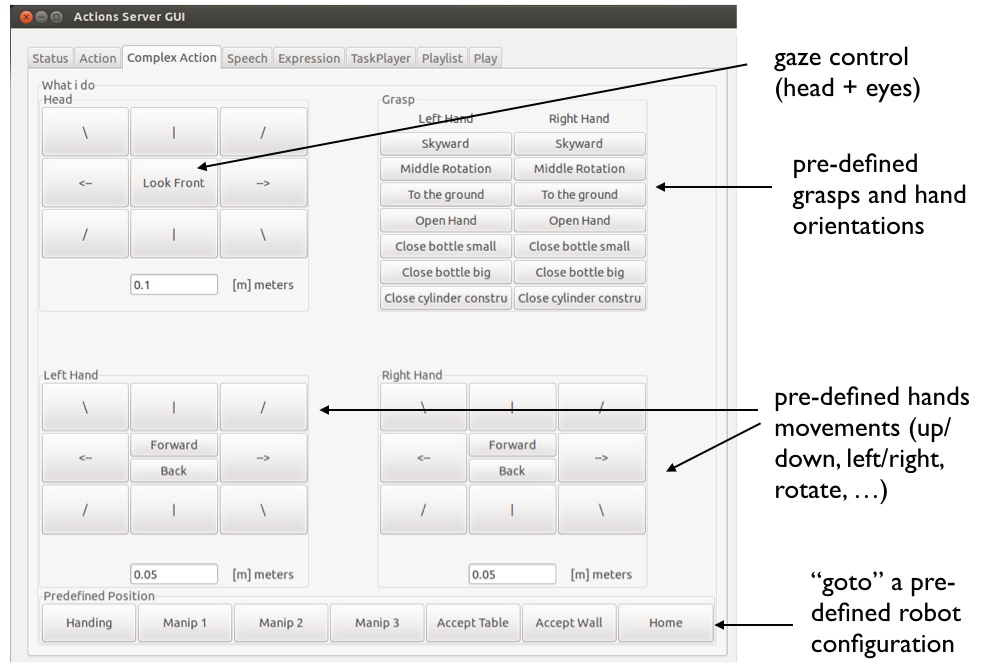
\includegraphics[height=7cm]{Serena/figures/gui_actions.jpg} \hspace{0.5cm}
{\large \textbf{\textsf{B}}} 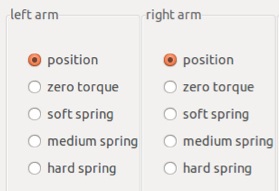
\includegraphics[height=2.5cm]{Serena/figures/gui_demoforcecontrol.jpg}
\caption{WoZ GUI. \textbf{\textsf{A}}: the tab dedicated to the quick control of gaze, grasps and hands movements in the Cartesian space. The buttons sends pre-defined commands to the \textit{actionsServer} module, developed in \cite{Ivaldi2014tamd}. The buttons of the bottom row allows the operator to bring the robot in pre-defined postures (whole-body joint configurations): they were pre-programmed so as to simplify the control of the iCub during the experiments, in case the operator had to ``bring it back'' to a pre-defined configuration that could simplify the interaction for the participants. They were useful also for prototyping and testing of the experiments. \textbf{\textsf{B}}: part of the GUI dedicated to switching the control mode of the arms -- position, zero-torque, then impedance control with low, medium and high stiffness.}
\label{fig:guiactions}
\end{figure*}


\begin{figure*}
\centering
{\large \textbf{\textsf{A}}} 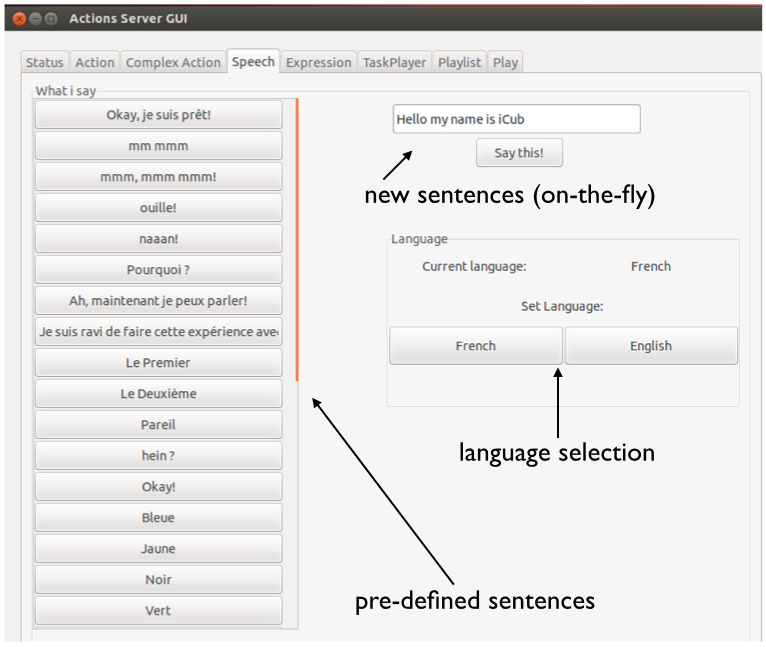
\includegraphics[height=6cm]{Serena/figures/gui_speech.jpg} \hspace{0.5cm}
{\large \textbf{\textsf{B}}}  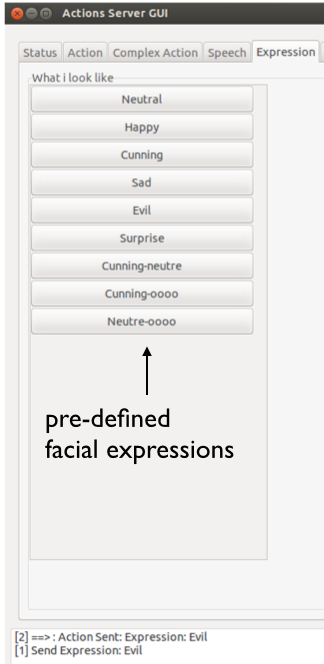
\includegraphics[height=6cm]{Serena/figures/gui_faceexpressions.jpg}
\caption{WoZ GUI. \textbf{\textsf{A}}: the tab related to the robot's speech. The operator can choose between a list of pre-defined sentences and expressions, or he can type a new sentence on-the-fly: this is done to be able to quickly formulate an answer to an unexpected request of the participant. The operator can switch between french and english speech (at the moment, the only two supported languages), even if in the experiments of this paper of course the robot was always speaking french. \textbf{\textsf{B}}: the tab related to facial expressions. The list of facial expression along with their specific realization on the iCub face (the combination of the activation of the LEDs in eyelids and mouth) is loaded from a configuration file.}
\label{fig:guispeech}
\end{figure*}


%\begin{acknowledgements}
%The authors wish to thank Charles Ballarini for his contribution in software and experiments, Salvatore Anzalone and Ilaria Gaudiello for their contribution to the design of the experimental protocol.
%\end{acknowledgements}

\clearpage{}

\chapter{A Shared Control Method for Online Human-in-the-Loop Robot Learning Based on Locally Weighted Regression}\label{sec:Luka}
\setcounter{figure}{0}
%\title{\LARGE \bf A Shared Control Method for Online Human-in-the-Loop Robot Learning Based on Locally Weighted Regression}

%\author{Luka Peternel$^{\text{a},}$$^{\text{c}}$, Erhan Oztop$^{\text{b}}$ and Jan Babi\v{c}$^{\text{c}}$% <-this % stops a space
%\thanks{$^{\text{a}}$HRI$^2$ Lab, Dept. of Advanced Robotics, Istituto Italiano di Tecnologia, Genoa, Italy, Email: luka.peternel@iit.it}
%\thanks{$^{\text{b}}$Robotics Laboratory, \"{O}zye\u{g}in University, Istanbul, Turkey}
%\thanks{$^{\text{c}}$Dept. of Automation Biocybernetics and Robotics, Jo\v{z}ef Stefan Institute, Ljubljana, Slovenia}
%\thanks{This work was supported by the EC Framework Programme 7 through the CoDyCo project (\#600716) and the Converge project (\#321700).}}


\subsection{Introduction}
\label{sec:introduction}
Robot learning can be a good alternative to time-consuming classical manual programming that requires experts and expert time. One such example is reinforcement learning where the robot autonomously learns the task through the trial-and-error principle \cite{Kober2012}. Another example is learning-by-demonstration where the human directly demonstrates the robot how to perform a given task \cite{Hersch2008,Evrard2009,Ude2010,Amor2009,Nguyen2009,Peternel2013b,Gams2009,Peternel2014}.

Robot learning-by-demonstration can be generally divided into offline and online type of learning \cite{Nguyen2011}. In offline learning the training data is acquired in the demonstration stage, and subsequently the training data is used in combination with a machine-learning method to form a robotic skill, which can be later used by the robot in the autonomous stage \cite{Hersch2008,Evrard2009,Ude2010,Ewerton2015}. The advantage of this approach is that the demonstrator can select the best data or adjust it in order to achieve the best learning performance. The key drawback of pure offline learning in the teaching-by-demonstration framework is that the human demonstrator does not have any feedback about the robot learning {\it during} the demonstration stage. The actual performance of the obtained robotic skill by using the data collected during demonstration can only be observed later in the autonomous stage. If the autonomous performance is unsatisfactory then the whole procedure has to be repeated.

Above-mentioned drawback can partially be addressed by multiple demonstrations to obtain some variety that can benefit the obtained robotic skill during the autonomous stage \cite{Ewerton2015}. Alternatively, the skill obtained during the demonstration stage can be corrected by the human in the autonomous stage through social interaction \cite{Nicolescu2003,Lockerd2004,Argall2007}. However, this method requires relatively high level of robot intelligence to recognise the human advice and devise a strategy to correct its performance on sensorimotor level. If the task is complex, the correction procedure may be time-consuming and in some cases unsuccessful. Therefore, another direct sensorimotor-level demonstration from the human could be faster and more efficient.

Contrary to offline learning, in online learning the robotic skill is formed gradually already during the demonstration stage \cite{Nguyen2011}. One of the advantages of this is that the transition between demonstration stage and autonomous stage can be direct and automatic \cite{Peternel2013b,Gams2009,Peternel2014}. Importantly, online learning also allows the demonstrator to get useful feedback about the performance of the robotic skill being constructed during the demonstration \cite{Lee2011,Peternel2013b,Peternel2016}. In this case, the correction of the obtained skill can be performed online and directly on sensorimotor level \cite{Lee2011,Peternel2016}, and it can therefore be faster and less complicated from the user perspective.

In \cite{Lee2011}, the authors proposed a kinaesthetic teaching method that allows the demonstrator to incrementally improve the the currently leant robotic skill. The skill refinement is done by physical interaction at low robot stiffness. However, in kinaesthetic teaching the immersion of demonstrator is limited, especially with regards to tactile sensing. In addition, simultaneous online demonstration of impedance \cite{Peternel2014,Peternel2015} can be difficult. These drawbacks can be addressed by teleoperation-based teaching \cite{Evrard2009,Peternel2013b,Peternel2014}. However, in this approach the control commands for the robotic mechanism are simultaneously generated by both the human demonstrator and by the robot control policy (represented as a non-linear function approximator) being learnt \cite{Peternel2013b}. Therefore, a mechanism that arbitrates the control responsibility over the target robotic platform is required to enable the co-adaptation between the involved agents.

\subsection{Related Work}
\label{sec:related}
While shared control is a well-studied subject in teleoperation \cite{Niemeyer2008,Dragan2013} and assistive robotics \cite{Omalley2006,Dragan2013,Jain2015,Peternel2016}, there are only a few studies that investigated shared control on a sensorimotor level in the teleoperation-based human-in-the-loop robot teaching. Study in \cite{Peternel2013b} proposed a method to share the control between the demonstrator and robotic skill in an online robot learning scenario based on Locally Weighted Regression (LWR) \cite{Schaal1998,Vijayakumar2005} machine learning. The control-sharing algorithm defined the amount of control responsibility of each agent as a ratio based on the prediction error, i.e. the average error between the human generated motor output and LWR output. The reasoning was that when the machine-learning algorithm learns to replicate human generated motor commands reliably then the control could be shifted to the machine control. This works very well when the demonstrator quickly becomes an expert in performing the task at hand \cite{Peternel2013b}.

Study in \cite{Zamani2015} developed a variant of the approach proposed in \cite{Peternel2013b} by designing a new strategy for determining the control arbitration. Instead of using prediction error to adjust the control sharing, they used a local success measure of the task execution, which does not directly depend on the prediction error of the machine-learning module. This is beneficial for tasks where the human demonstrator needs time to adapt to task to perform well; because this does not allow the machine to learn a bad policy by simply becoming a very good imitator of a bad demonstrator. The local success measure is somewhat analogous to introducing virtual rewards to speed-up learning in the reinforcement-learning framework. The disadvantage of this approach is the additional complexity and task dependency. For a useful local success measure the task must be well defined and should naturally facilitate local success definition, by for example, allowing state space decomposition into subtasks. Naturally, some tasks do not meet these conditions, and for those that meet, the one-time expert effort might be non-negligible.

The two approaches in \cite{Peternel2013b} and \cite{Zamani2015} described above both advocate a control sharing mechanism between the agents. This means the performance of the robot during demonstration is a mixture of human and machine control. Here we have two potentials difficulties for the human demonstrator. (1) The credit assignment problem: it may be difficult to determine whether the current unsatisfactory performance of the robot is due to the control commands from the demonstrator or the machine-learning module. (2) The non-stationarity problem: how the robot responds to the human control commands that change with time and in a complex way; this must be an initial burden for human demonstrators \cite{Zamani2015}.

In this paper we propose and investigate a new shared-control approach for teleoperation-based human-in-the-loop online robot teaching that addresses the two difficulties indicated above. Contrary to \cite{Peternel2013b} and \cite{Zamani2015}, we adopt a binary control responsibility scheme where the control is either fully delegated to the demonstrator or to the machine-learning module. This allows the demonstrator to clearly know who is responsible for the ongoing task execution performance. In addition, the approach retains the simplicity from the user perspective \cite{Peternel2013b} as it does not require the task and reward function to be defined in advance. In \cite{Peternel2013b} the control is delegated gradually based on the average error between the human and robotic skill performance over the entire state space up until the current observation time. The disadvantage of this is that human cannot efficiently inspect the robotic skill performance locally in a specific state region. Contrary to that, in the proposed method the control is delegated based on the existence of local models in specific state regions. This gives the demonstrator an option to freely inspect the performance of the robotic skill in any specific state region (and if necessary to correct it).

\subsection{Methods}
In the proposed approach, the control sharing is based on a mechanism that exploits the machine-learning method (LWR) adopted \cite{Schaal1998,Vijayakumar2005}. LWR builds a non-linear model by creating local linear models over non-linear basis functions that have local span (i.e. receptive fields) over the states and are incrementally generated during task demonstration. The existence or nonexistence of local models (in the LWR module) in a given state region is used to arbitrate control: when the robot finds itself in a state region where no local models exist the control is given to the human demonstrator so that new models can be learnt. If the current state of the robot is within the proximity of a local model (i.e. it activates the receptive field of some model) then the control is given to the machine-learning module. This allows the human to examine the performance of the current robotic skill during the demonstration stage. If the performance is unsatisfactory the teaching can be repeated and models can be updated/replaced in the given state region.
\begin{figure}[!t]
  \centering
  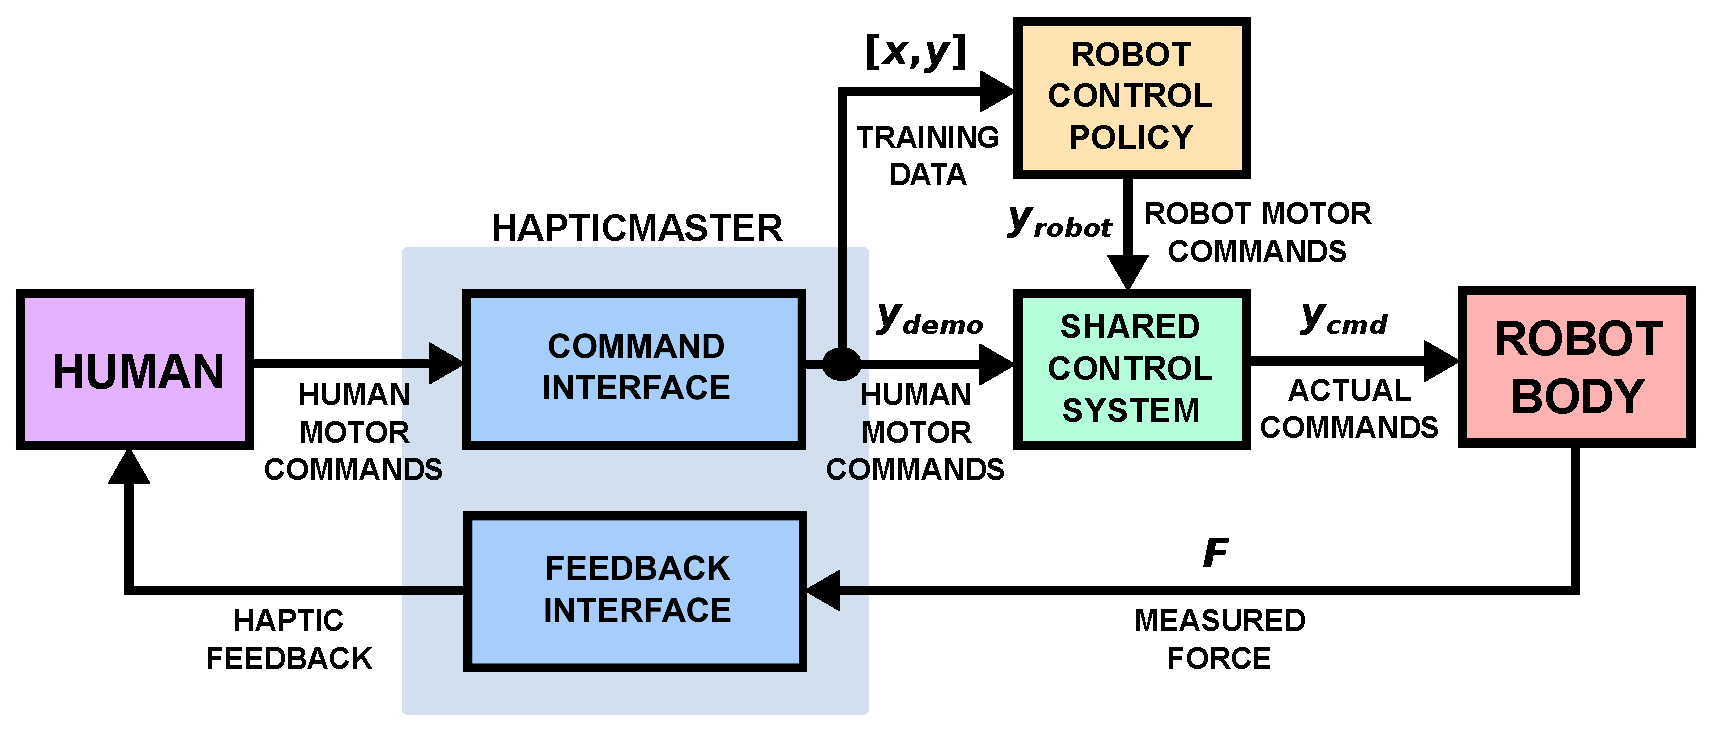
\includegraphics[width=0.70\textwidth]{Luka/scheme.eps}
  \caption{The proposed human-in-the-loop teaching approach with shared control between the actions of demonstrator ($y_{demo}$) and robotic skill ($y_{robot}$). HapticMaster robot serves as an interface between the demonstrator and the controlled robotic manipulator.}
  \label{fig:scheme}
  \vspace{-4 mm}
\end{figure}

To demonstrate and validate the concept of the proposed method we performed experiments on a Moog HapticMaster (HM) robot. The task of the robotic manipulator was to produce a reference force between its end-effector and unknown objects in the environment. The surfaces of the objects had different stiffness. The task of the human demonstrator was to teach the robotic manipulator how to adjust the commanded (reference) position in order to maintain the predefined force over the entire operational space (plane).

The human demonstrator was included into the robot control loop by a human-robot interface as shown in Fig. \ref{fig:scheme}. The HM robot served as the necessary control interface for the virtual robotic manipulator that needs to be manoeuvred to achieve a constant vertical force feedback over an environment that has non-homogenous stiffness. While operating the robot trough this teleoperation setup, the human demonstrator could easily gain the skill to perform the task through the robot. After an initial practice session, the skill demonstration stage was started where the human demonstrator taught the robot how to perform the desired task. Simultaneously, the robot acquired the skill incrementally in real-time as detailed below. The proposed control arbitration mechanism delegated the control to the demonstrator or to the so-far-built robot control policy (robotic skill). The control policy learning was inhibited for the state regions where sufficient level of learning was already attained, and the robot was commanded using this learnt policy. In contrast, when the robot entered a state region where sufficient learning did not take place, the control was granted to the demonstrator and the learning resumed.


\subsubsection{Locally Weighted Regression}
The LWR method\footnote{LWR is used here for generality. Locally Weight Projection Regression\cite{Vijayakumar2005} can be used in our method instead to cope with higher dimensionality.} is an incremental (online) function approximator that can be used to represent {\it output} as a function of {\it input} given a set of [input, output] pairs, i.e. the training data points. To do this, it forms local expert models that are responsible for particular input regions. Each local expert is a linear model and is assumed to represent its responsibility area. The output prediction $\hat{\bm{y}}(\bm{x})$, for some new input $\bm{x}$, is given by the sum of contributions of all local models \cite{Schaal1998}
\begin{equation}
\hat{\bm{y}}(\bm{x}) = \frac{\sum\limits_{i=1}^N w_{i}\bm{y}_{i}^{model}}{\sum\limits_{i=1}^N w_{i}},
\label{eq:lwr1}
\end{equation}
where $\bm{y}_{i}^{model}$ is the prediction of the $i^{th}$ local model, and $w_{i}$ its weight. Weights determine the contribution of each local model in the final prediction, $\hat{\bm{y}}$ given input $\bm{x}$. Weights are computed by the activation of models' receptive fields defined by Gaussian kernel functions \cite{Schaal1998}
\begin{equation}
w_{i} = \exp\big(-\frac{1}{2}(\bm{x}-\bm{c}_{i})^{T}\bm{D}_{i}(\bm{x}-\bm{c}_{i})\big),
\label{eq:lwr2}
\end{equation}
where $\bm{D}_{i}$ is positive definite matrix that contains information about the size of receptive field. Parameter $\bm{c}_{i}$ represents the centre of the receptive field and its local model. By observing (\ref{eq:lwr2}) one can notice that the influence (weight) of a local model $\bm{y}_{i}^{model}$ decreases with the distance of input $\bm{x}$ from the centre $\bm{c}_{i}$ of that model.

Local linear models are defined as \cite{Schaal1998}
\begin{align}
	\bm{y}_{i}^{model} &= (\bm{x} - \bm{c}_i)^{T} \bm{m}_i + m_{0,i} = \tilde{\bm{x}}_{i}^{T}\bm{M}_{i},\label{eq:lwr3}\\
	\tilde{\bm{x}} &= [(\bm{x}-\bm{c}_{i})^{T},1]^{T},\label{eq:lwr4}
\end{align}
where $\bm{y}_{i}^{model}$ is the i-th model prediction given the input $\bm{x}$, while $\bm{c}_{i}$ is the centre of the $i^{th}$ model. Vector $\bm{M}_{i}$ contains the parameters that describes the local model and $\tilde{\bm{x}}$ is the distance from the centre of the model.

The learning process needs to determine model parameters $\bm{M}_{i}$, centre parameters $\bm{c}_{i}$ and distance metrics $\bm{D}_{i}$ that determines the size of the model's receptive field. The learning is done incrementally while the training data are fed to the learning system. Each training data point $[\bm{x},\bm{y}]$ updates the existing models via  recursive least-square method \cite{Schaal1998}
\begin{align}
\bm{M}(k+1) &= \bm{M}(k) + w \bm{P}(k+1) \tilde{\bm{x}} \bm{e}_{lwr}^{T},\label{eq:lwr5} \\
\bm{e}_{lwr} &= (\bm{y}-\bm{M}(k)^{T}\tilde{\bm{x}}),\label{eq:lwr6} \\
\bm{P}(k+1) &= \frac{1}{\lambda}\left(\bm{P}(k)-\frac{\bm{P}(k)\tilde{\bm{x}}\tilde{\bm{x}}^{T}\bm{P}(k)}{\frac{\lambda}{w}+\tilde{\bm{x}}^{T}\bm{P}(k)\tilde{\bm{x}}}\right) ,\label{eq:lwr7}
\end{align}
where $\lambda$ forgetting factor that allows the system to gradually forget the previously demonstrated training data points.

Adjustment of model's receptive field size is performed by a modified leave-one-out cross-validation method \cite{Schaal1998}. As new training data points are used for the LWR update, new local models are created - and in same cases removed, to facilitate a parsimonious distribution of the local models across the input space. A new model is created when a training point $[\bm{x},\bm{y}]$ does not active any of the receptive fields more than a threshold $w_{gen}$ \cite{Schaal1998}, and the centre of the newly created model is set to the position of the new training point ($\bm{c}=\bm{x}$). When a training point activates two receptive fields simultaneously for more than a predetermined threshold $w_{prune}$, then the model with the larger covariance matrix is removed \cite{Schaal1998}. This prevents unnecessary overlap of the models that would lead to computational inefficiency.

\subsubsection{Shared-Control Approach}
We delegated the control over the robotic mechanism between the human and robotic skill by the following expression \cite{Peternel2013b} (see also Fig. \ref{fig:scheme})
\begin{equation}
\bm{y}_{cmd} = C \cdot \bm{y}_{demo} + (1-C) \cdot \bm{y}_{robot} ,
\label{eq:delegation}
\end{equation}
where $\bm{y}_{cmd}$ is a vector of commands sent to the robotic mechanism, $\bm{y}_{demo}$ is a vector of commands given by the human demonstrator, $\bm{y}_{robot}$ is a vector of commands produced by the current robotic skill and $C \in [0,1]$ is a weight factor that determines the influence of each agent. Pure human control is achieved when $C = 1$, and pure machine control is achieved when $C = 0$.

In our method, we used the information about the current state of the local models in LWR to determine the value of the factor $C$. When the demonstrator is performing the task in a state (i.e. position on the plane) where a feasible local model exists the task execution is purely based on the current robot control policy that is represented by (\ref{eq:lwr1}), and learning is inhibited. If no local model is present in the current robot state then the control of the task execution is given to the demonstrator, and teaching is resumed. To determine the proximity to the local model we used the activation $w_{max}$ of the model that provides the maximum activation for the current position of the input vector $\bm{x}$. We defined factor $C$ as
\begin{equation}
C = \begin{cases} 1 & \text{if } w_{max} < (w_{th} - \frac{d}{2})
\\ \frac{ 1 + \cos \big(\pi \frac{w_{max} - (w_{th} - \frac{d}{2}) }{d}\big)}{2}  & \text{if } (w_{th} - \frac{d}{2}) \leq w_{max} \leq (w_{th} + \frac{d}{2}),
\\ 0 & \text{if } w_{max} > (w_{th} + \frac{d}{2}) \end{cases}
\label{eq:factor}
\end{equation}
where $w_{max}$ is the strongest activation of the model receptive fields \cite{Schaal1998} and $w_{th}$ is an activation threshold that we introduced to determine the model-proximity based shared control. Although, the main regime for $C$ is binary, we used a cosine based function to prevent sudden jumps in net control output and to facilitate smooth transitions between human control and machine control modes of operation. Here the parameter $d$ defines the width of switching function, and thus should be assigned a small value to obtain the desired binary regime.

During the demonstration stage the training data is collected and accumulated for a predefined sample length before it is fed to the LWR-based learning system. Instead of feeding the data to LWR in the order it is received, a random order can improve the learning at lower $\lambda$. Data accumulation takes place only when the human demonstrator has control over the robot (i.e. control factor $C = 1$). When appropriate LWR models exist in a given state region, the robot behaves autonomously by following the control policy dictated by the active LWR models (i.e. control factor $C = 0$). The data accumulation is paused in this case, until when the user gains full control again. The described approach can be described as
\begin{equation}
\bm{A}_{new} = \begin{cases} \bm{A} & \quad \text{if } C \neq 1
\\ [\thinspace \bm{A}; \thinspace [\bm{x}, \thinspace \bm{y}]\thinspace ] & \quad \text{if } C = 1 \text{ \& } \text{length}(\bm{A}) < N_{acc},
\\ [\thinspace] & \quad \text{if } \text{length}(\bm{A}) = N_{acc} \\ \end{cases}
\label{eq:accumulate}
\end{equation}
\begin{equation}
\bm{A}_{in} = \bm{A}\big(\text{randperm}(N_{acc}),\thinspace :\big),
\label{eq:shuffle}
\end{equation}
where $\bm{A}$ is the matrix (accumulation buffer) where the training data is accumulated, and the notation $\bm{A}_{new}$ indicates that $\bm{A}$ is updated at each iteration. $N_{acc}$ is the predefined accumulation sample length that determines the amount of data that is fed to LWR in each update epoch. As mentioned above, a shuffling is applied before the data is fed to LWR, so instead of $\bm{A}$, $\bm{A}_{in}$, the random shuffled version of it is used. If we want to accumulate a large data set before each update then it is reasonable to reduce its size by also applying down-sampling before the shuffling.

The final transition from the demonstration stage to the fully autonomous stage (human demonstrator disconnected from the robot control loop) can be either done automatically or manually. The automatic switch can be realised based on the threshold percentage of the given task space being covered by the local models.


\subsection{Experimental Setup}
In the experiments we used HM robot as an interface between the human demonstrator and the robotic manipulator (see Fig. \ref{fig:setup}). Please refer to the supplementary multimedia file for a video of the setup/experiment. HM has a robotic arm with 3 active degrees of freedom that can render a haptic environment at the end-effector where the human holds and moves it. At the same time HM provides the measured position of the end-effector that can be used to command the position of the teleoperated robotic manipulator. The physical aspects of the robotic manipulator and the environment were simulated in MATLAB/Simulink, while the visual aspects were simulated by the OpenGL Utility Toolkit (GLUT) (see Fig. \ref{fig:surface}). The robot was positioned in front of the demonstrator who sat on a chair. We mounted a monitor in front of the demonstrator where we displayed the virtual environment and feedback related to the task execution. The machine-learning algorithm was based on the toolbox provided by \cite{Klanke2008}. The learning and shared-control algorithm operated at 100 Hz.
\begin{figure}[!t]
  \centering
  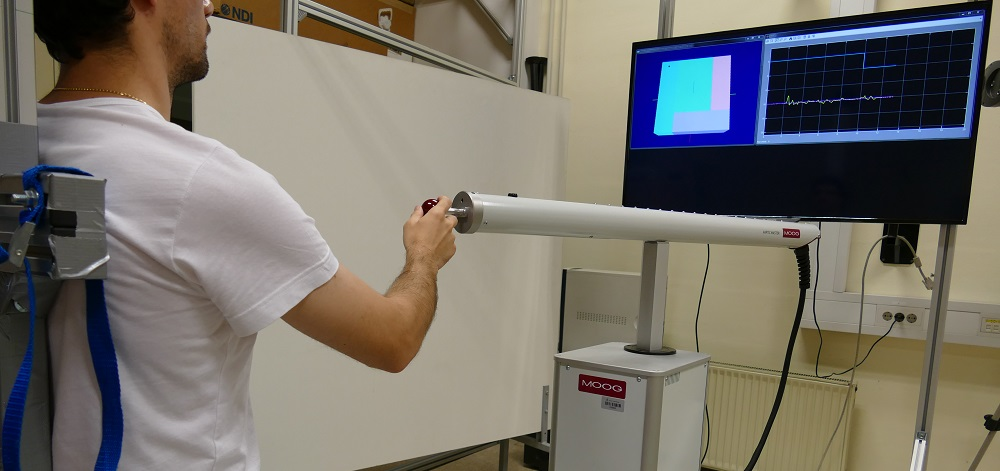
\includegraphics[width=0.6\textwidth]{Luka/setup.jpg}
  \caption{Robot manipulator control interface consisting of HapticMaster robot and monitor for providing human with visual feedback.}
  \label{fig:setup}
  \vspace{-2 mm}
\end{figure}
\begin{figure}[!t]
  \centering
  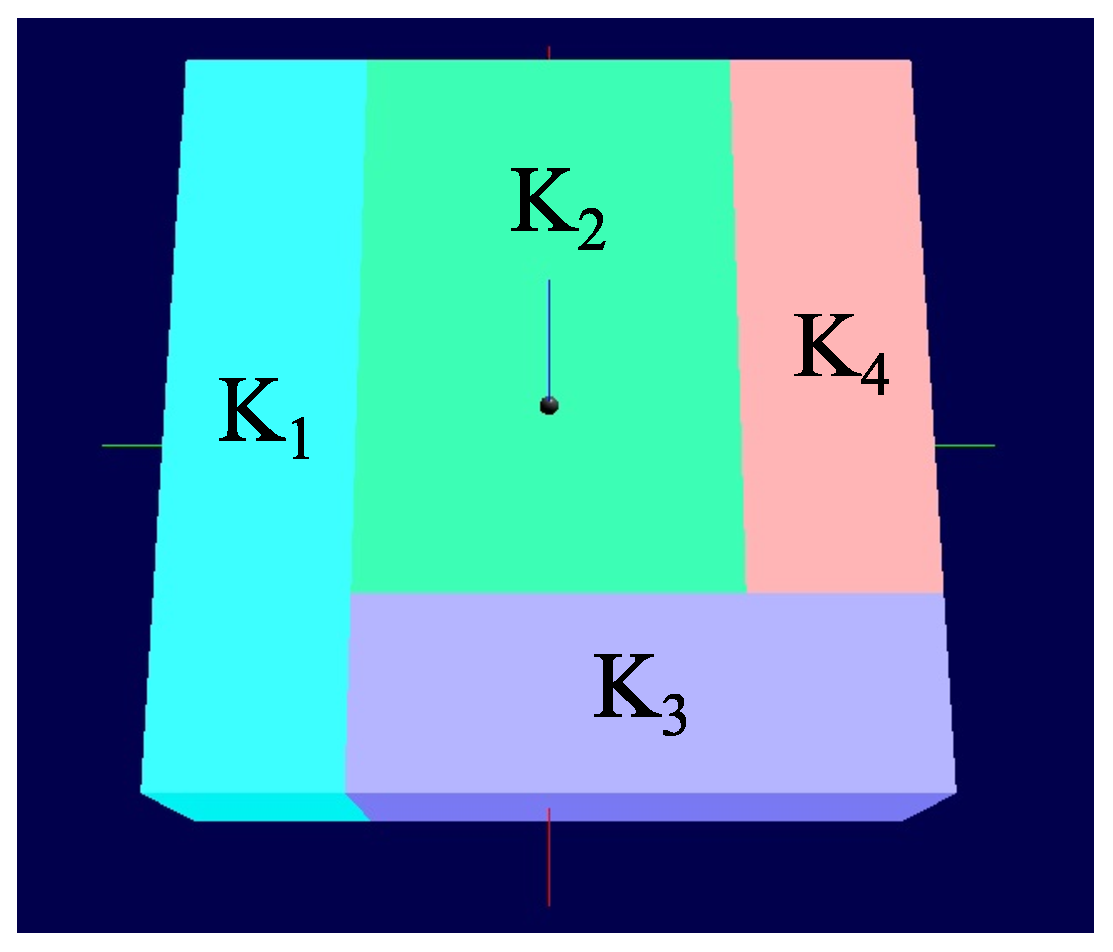
\includegraphics[width=0.4\textwidth]{Luka/env.eps}
  \caption{Virtual environment. The colours represent different objects on the surface. Each object has a different stiffness ($K_1$, $K_2$, $K_3$ and $K_4$). The robotic manipulator's actual end-effector position is displayed by the black ball in the centre.}
  \label{fig:surface}
  \vspace{-4 mm}
\end{figure}

The HM robot operated in two modes. The first mode was admittance control where the measured interaction force between the HM end-effector and human hand produced the desired motion. This mode was used in case when the demonstrator had the control over the virtual robotic manipulator ($C=1$). The actual position of the HM end-effector (human demonstrator's arm end-effector) was used as the commanded (reference) position for the virtual robotic manipulator. The actual position of the manipulator was dependant on the surface in the virtual environment. We assisted the demonstrator in precise maintaining the desired commanded position in z-axis by a virtual spring-damper system. The second mode was position control using a proportional controller realised by a virtual spring between the reference and actual HM end-effector position in z-axis. This mode was used in case when the robotic skill had the control over the virtual robotic manipulator ($C=0$).

One experienced human demonstrator participated in the experiments. The task of the robotic manipulator was to produce a reference interaction force on the unknown objects in the environment. The interaction force had to be produced perpendicularly to objects (in z-axis). Each object had different stiffness properties. To maintain the desired force the demonstrator had to adjust the commanded (reference) end-effector position in z-axis of the robotic manipulator based on the position in x-y plane. Please note that variables $x$ and $y$ now correspond to the position of robotic manipulator's end-effector. The following equation describes the necessary force control policy
\begin{equation}
	F_{z} = K(x,y) \big(z_r-z_a\big),\label{en:robotimp}
\end{equation}
where $F_{z}$ is the interaction force acting between the manipulator and the environment in z-axis, $K(x,y)$ is the stiffness of the object in z-axis, $z_a$ is actual and $z_r$ is reference position of the manipulator's end-effector in z-axis. The stiffness $K(x,y)$ depends on the object (i.e. on the position in x-y plane). Actual position $z_a$ depends on the environment too as the object blocks it from reaching the reference position inside the object. The higher the desired force is at a given stiffness of the object the larger the difference between commanded and actual position must be (i.e. reference must be deeper inside the object). For producing the same force, the difference between the commanded and actual position must be lower for objects with higher stiffness and vice-versa.

\begin{figure*}[!ht]
  \centering
  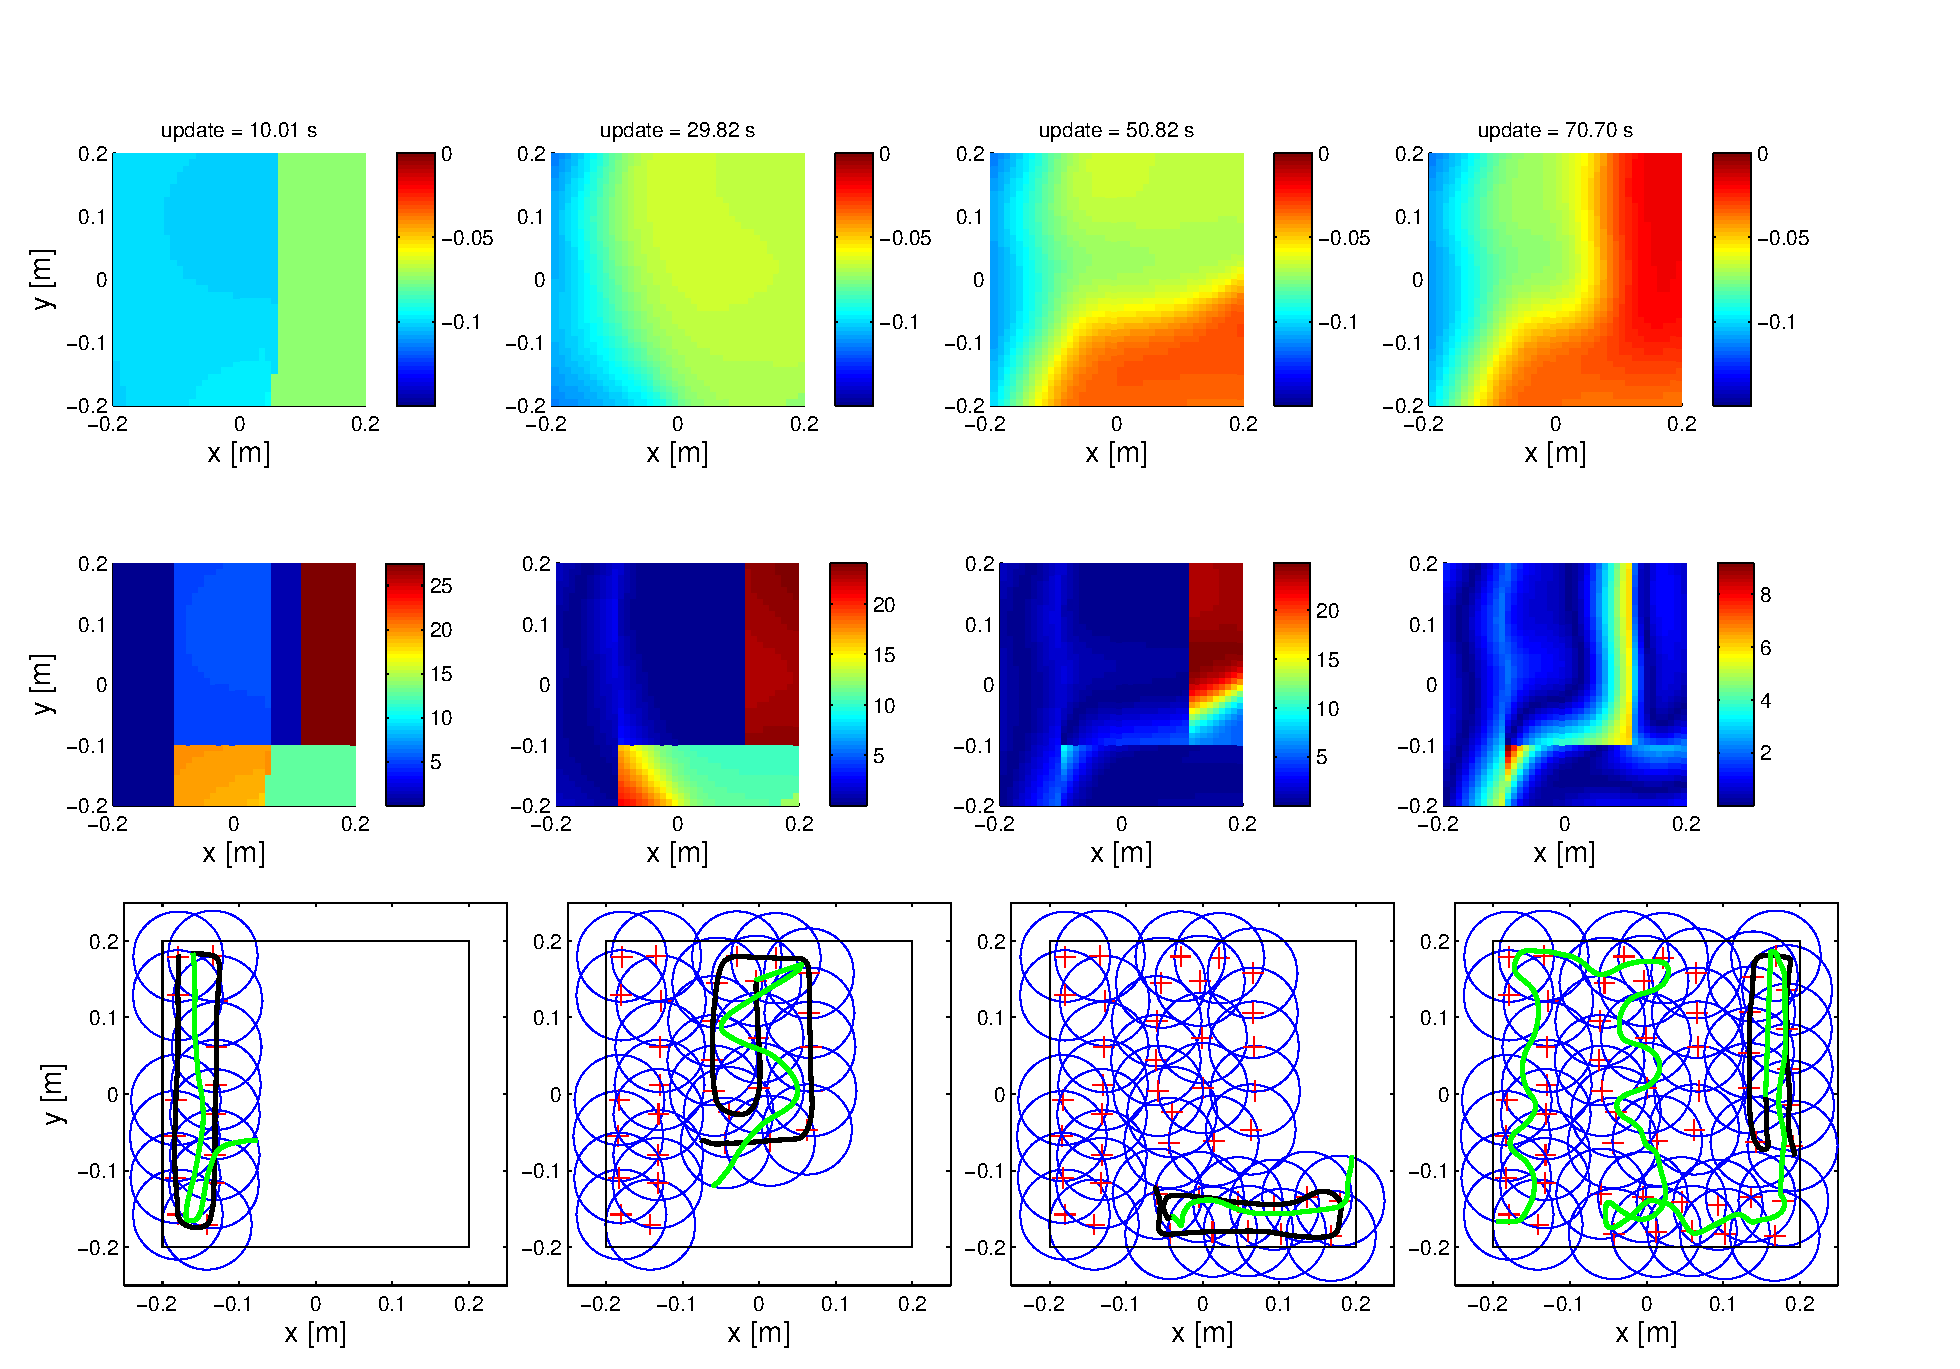
\includegraphics[width=0.85\textwidth]{Luka/results1.eps}
  \caption{Results of the experiments - learning. The top row graphs show prediction of robotic manipulator's commanded (reference) position displacement from the actual position in z-axis. The middle row graphs show the error of predicted interaction force in z-axis. The bottom row graphs show the motion trajectory in x-y plane (thick black line corresponds to $C=1$, thick green line corresponds to $C=0$) and distribution of local models (red crosses are centres and blue ellipses are activation ranges of $w_{th}$). Each column represents the state of robotic skill after training data update (update time stamps are on the top).}
  \label{fig:models}
  %\vspace{-4 mm}
\end{figure*}

We constructed a $0.4$ by $0.4$ meter surface from four different objects. The configuration of surface is shown in Fig. \ref{fig:surface}. Each object had a different stiffness: $k_1=100$ N/m, $k_2=150$ N/m, $k_3=300$ N/m and $k_4=500$ N/m. The goal was to teach the robotic manipulator how to produce a reference force $F_z=10$ N (LWR output) perpendicularly to the surface regardless of the position on the x-y plane (LWR input). The human demonstrator had to move the manipulator's position on x-y plane across various parts of the surface and the commanded position in z-axis had to be adjusted so that the reference force was maintained according to (\ref{en:robotimp}). While doing this, the learning system gradually acquired the skill how to produce the task autonomously. If the models existed in the given state region of x-y plane the shared-control system delegated the control responsibility over the manipulator to the robotic skill. Otherwise, the demonstrator had the control in order to continue the teaching process.

We determined parameters for the LWR-based learning system experimentally. The parameter related to the size of the model was set to $\bm{D} = \begin{bmatrix} 400 & 0 \\[0.3em] 0 & 400\end{bmatrix}$. The values of diagonal elements correspond to each input. Since in our case the inputs are the same physical quantity (position in x and y-axis), we set both diagonal elements to equal value. In case the inputs are different physical quantities then the values should be appropriately set for each input separately. Parameters related to the generation and removal of the models were set to $w_{gen}=0.8$, $w_{prune}=0.9$. For these proof-of-concept experiments selected $\lambda=1$ since we did not want to forget the old training data. If forgetting of older data is preferred then $\lambda < 1$ should be used.
\begin{figure*}[!ht]
  \centering
  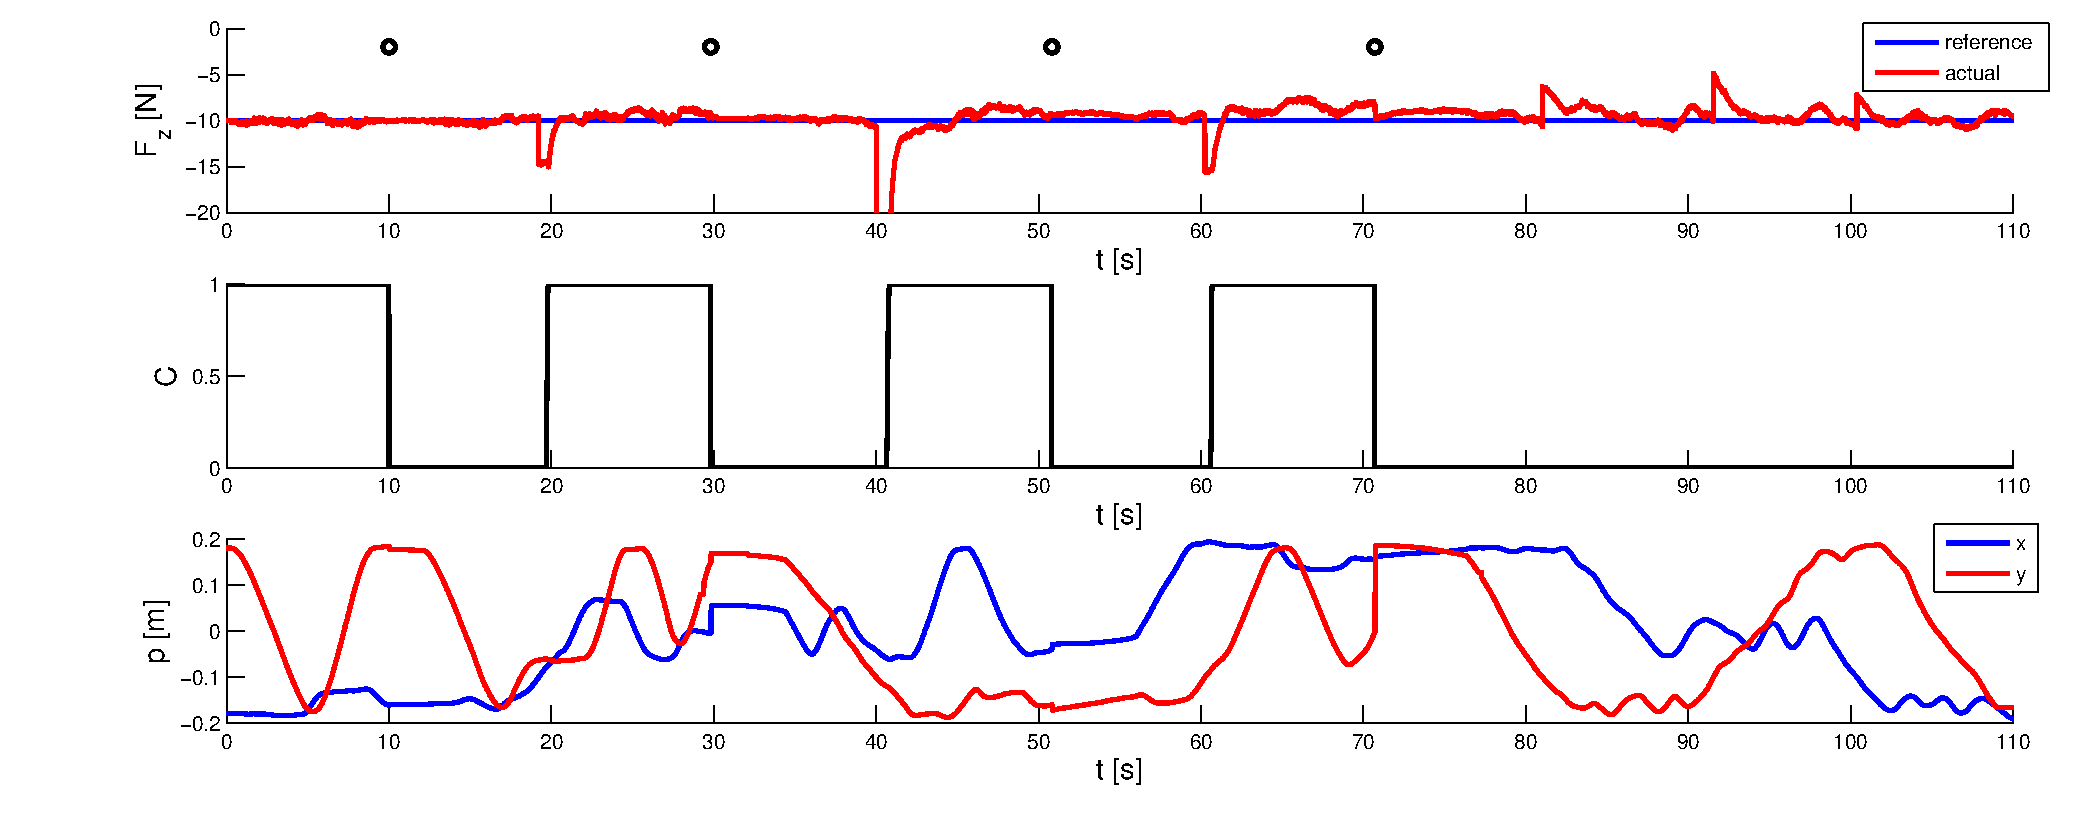
\includegraphics[width=0.85\textwidth]{Luka/results2.eps}
  \caption{Results of the experiments - task execution and shared control. The top graph shows the reference and actual force in z-axis. The middle graph shows the control responsibility factor $C$ (1 = demonstrator, 0 = robotic skill). The bottom graph shows the position of the manipulator in x-y plane. Training data updates are indicated by black dots on the top and correspond to the time stamps at the top of Fig. \ref{fig:models}.}
  \label{fig:force}
  \vspace{-4 mm}
\end{figure*}

The parameters for shared-control system were also set experimentally. The threshold of model's receptive field activation that determines whether the control is given to the demonstrator or robotic skill was set to $w_{th}=0.5$. We recommend following $w_{th}\leq w_{gen}$ in order not to create new models while the demonstrator does not have the control responsibility. The parameter related to smooth transition of control responsibility between the human and robotic skill was set to $d=0.05$. If slower transition phase is preferred then this parameter should be increased. Accumulation buffer length was set to $N_{acc}=1000$. This parameter should be lower if more frequent updates of robotic skill are preferred.

\subsection{Results}
The results of the robot learning during the experiment are shown in Fig. \ref{fig:models}. Each column represents the different stage of training data update. The time stamps of the update application are displayed on the top. The top row shows the acquired models (robotic skill) for manipulator's displacement of reference position from the actual position in z-axis. The middle row shows the force prediction error of the models at each stage. The bottom row shows the motion of the robot manipulator (thick black and green line) on the object's surface (thin black rectangle). The black line shows the trajectory when the demonstrator had the control over the robotic manipulator's force production task. The green line shows the trajectory when robotic skill had the control over the robotic manipulator's force production task. The red crosses show the centres while blue ellipses show the threshold activation ranges $w_{th}$ of the currently available local models that are part of robotic skill.

From the graphs we can see how the overall model was gradually updated when the demonstrator was teaching at various sections of the surface. In the first stage the local models are only created around the state region where the demonstration was initially performed. In the other sections of the surface the prediction error is naturally high due to non-existence of local models. When the demonstration progressed additional models were generated in the other sections. In the last training data update the local models fully covered the space of the given task and the robotic manipulator entered the fully autonomous stage (i.e. autonomously produced the desired force based on the position on the x-y plane).

Additional results are shown in Fig. \ref{fig:force}. The interaction force control as a result of adjusted commanded (reference) position along z-axis is shown in the top graph. We can see that the desired force was maintained relatively well by both the demonstrator and the obtained robotic skill. The black dots in the top show the time stamps when the training data was updated and correspond to the update times in Fig. \ref{fig:models}. The control responsibility factor $C$ is shown in the middle graph. The position of the manipulator in x and y-axis is shown in the bottom graph. Initially, $C$ was equal to one as there were no models present. After the prescribed amount of training data $N_{acc}$ was accumulated the robotic skill was updated with the learnt models in the demonstrated state region. Demonstrator then remained in that state region to examine the performance of the obtained robotic skill. Consequently $C$ became zero to give the control responsibility to the robotic skill. This procedure then repeated for the remaining three state regions of the task defined by different stiffness of the plane.

By observing the control responsibility we can see how it switched from demonstrator to the currently available local models. After each model update the control responsibility was shifted from the demonstrator to the robotic skill as the current position of robotic manipulator was within the predefined range of the existing models ($w_{max}>w_{th}$). The demonstrator could then move within the area where the teaching was already done to observe how the obtained robotic skill performs the task autonomously (see thick green lines in bottom graph of Fig. \ref{fig:models}). When the validation was done, the demonstrator moved to the unexplored area to perform the teaching there (see thick black lines in the bottom graph of Fig. \ref{fig:models}).


\subsection{Discussion}
The aim of this paper was to propose a new shared-control approach for human-in-the-loop robot teaching, and realise it for a non-trivial task as a proof-of-concept. In the hardware experiments conducted, the demonstrator could examine, online, the performance of the robotic skill being built during the demonstration stage, and gradually transform the robot to be an expert in the full allowed workspace. In the current implementation, we did not implement the ability of the demonstrator to remove already built local models. This was not needed in the current experiments as the demonstrator was expert and did not teach {\it bad} policies. This feature can be incorporated into the current system as a manual interface (e.g. pushing a button) or an automatic mechanism that detects the demonstrator's effort to correct a bad policy.

In future we will introduce an upgrade to the proposed framework where the human demonstrator will be able to remove the models, if the robotic skill performance is unsatisfactory after online examination. This will clear the undesired models in designated state region and allow corrections by re-teaching. Parameter $\lambda$ could be used in this case to forget the undesired models. In addition, we will experimentally explore the influence of system parameters on the performance of the proposed method.

By observing the obtained models in Fig. \ref{fig:models}, we can see that there is a considerable prediction error on the borders between two objects of different stiffness. This can be attributed to the difficulty of regression method to model larger discrete transitions within the training data output.

Potential disadvantage of the proposed method compared to \cite{Peternel2013b} and \cite{Zamani2015} is that the demonstrator has to manually inspect and determine the quality of the robotic skill. However, this gives the demonstrator more control over the learning. In addition, no extra cost functions are required to determine the quality automatically, as they can be hard to acquire and can produce unreliable results in complex tasks.
\clearpage

\chapter{Stepping in a novel balance environment}\label{sec:Zrinka}
\setcounter{figure}{0}

\subsection{Introduction} 
High stepping reaction time is a predictor of future falling \cite{Lord2001}, possibly due to inadequate weight shifts preceding foot lift-off \cite{Cohen2011}\cite{Sparto2013}. These can occur due to external balance perturbations \cite{Mille2014} or incorrect planning \cite{Cohen2011}\cite{Sparto2013}. Thus, incorrect weight shift planning might be linked to falls \cite{Robinovitch2013}. To investigate the effect of incorrectly scaled weight shifts on stepping, we developed a novel robotic platform able to amplify subjects’ weight shifts in real-time.

\subsection{Methods}
Eleven young adults (23.7$\pm$4.6 years) stepped as fast and accurate as possible to a target suddenly illuminated in front of one of their legs. On 1/3 of the steps the target jumped shortly before foot liftoff, forcing quick and potentially destabilizing adjustments. This task was performed on a moveable platform in three conditions: platform still (baseline, 60 steps and post-adaptation, 30 steps) or moving (adaptation, 90 steps). When moving, the platform doubled subjects’ mediolateral center of mass movement (COM) in real time. Thus, subjects had to plan a smaller COM movement to generate a weight shift appropriate for stepping to targets.
We calculated stepping errors (distance between the target and the foot at landing), step onset time (time between target onset and foot liftoff) and step execution time (time between liftoff and landing). Overall performance was analyzed using rANOVA (target jump x condition) and differences between the first and last five steps of each condition using paired samples t-tests.

\begin{figure*}[!ht]
	\centering
	\includegraphics[width=0.6\linewidth]{"Zrinka/methods"}
	\caption{Experimental setup. The subject is standing on a movable platform and a lighted area appears on the floor in front of his leg, serving as a stepping cue and target.}
	\label{fig:expSetup}
	\vspace{-4 mm}
\end{figure*}

\subsection{Results}
Target jumps increased step execution times and stepping errors (by 50 ms and 49.5 mm, both p $<$ .01).  Step onsets were delayed in adaptation (by 7 ms), but faster in post-adaptation (by 24 ms). Target jumps delayed step onset by 10 ms in baseline and adaptation (condition x jump interaction, p = .03). Step onsets were faster in the first 5 steps of post- adaptation, compared to last adaptation steps (by 37 ms, p = .01, jump). Stepping errors increased at the start of adaptation (by 19.5 mm, p = .02, no jump), but decreased over time, within adaptation (by 21.8 mm, p = .03, target jump) and post- adaptation (by 7.5 mm, p = .047, no jump).

\begin{figure*}[!ht]
	\centering
    \includegraphics[width=0.6\textwidth]{"Zrinka/step error-all steps"}
	\caption{Stepping errors. Error bars indicate standard deviation. Statistics are given in the text.}
	\label{fig:stepErrorAll}
\end{figure*}

\begin{figure*}[!ht]
	\centering
	\includegraphics[width=0.6\textwidth]{"Zrinka/step onset time-all steps"}
	\caption{Step onset time (time from the cue to step to foot lift-off). Error bars indicate standard deviation. Statistics are given in the text.}
	\label{fig:stepOnsetTimeAll}
\end{figure*}

\begin{figure*}[!ht]
	\centering
	\includegraphics[width=0.6\textwidth]{"Zrinka/step exec time-all steps"}
	\caption{Step execution time (time from step onset to landing). Error bars indicate standard deviation. Statistics are given in the text.}
	\label{fig:stepExecTimeAll}
\end{figure*}

\subsection{Conclusions}
When targets jumped, stepping errors increased, but manipulating balance by platform movements had no effect on stepping accuracy. However, manipulating balance delayed step onsets, in line with the need to adjust weight shifts prior to foot liftoff in this novel environment, and was accompanied by increased stepping errors in the first five steps. Although initially significantly perturbed, subjects quickly adapted to stepping in a novel balance environment. Analyses of weight shifting and adaptation rates of weight shifting and stepping to clarify the underlying mechanisms are pending.
\clearpage{}

\bibliographystyle{plain}
\bibliography{platform,IROS2016,edhhi,ChieBib}

\end{document}

%%% Local Variables:
%%% mode: latex
%%% TeX-master: t
%%% save-place: t
%%% End:
